\documentclass[a4paper,11pt,twoside,openright]{report}
\usepackage[spanish, es-tabla]{babel} 
\usepackage[utf8]{inputenc}
\usepackage[T1]{fontenc}
\usepackage{lmodern}

\renewcommand{\familydefault}{\sfdefault}


\usepackage{tabulary}
\usepackage{booktabs}
\usepackage{eurosym}
\usepackage{graphicx}


%espacio entre parrafos y sangria
\usepackage{parskip}
\setlength{\parindent}{1em}


%ENCABEZADOS Y PIES DE PAGINA
\setlength{\headheight}{15pt}

\renewcommand{\chaptermark}[1]{%
    \uppercase{
        \markboth{#1}{}}}

\usepackage{fancyhdr}
\fancypagestyle{plain}{%
    \fancyhf{}%
    \fancyfoot[RO,LE]{\thepage}%
    \renewcommand{\headrulewidth}{0pt}
}

\pagestyle{fancy}
\renewcommand{\chaptermark}[1]{%
    \uppercase{
        \markboth{#1}{}}}
\fancyhf{}
\fancyfoot[RO,LE]{\thepage}
\fancyhead[CO]{\leftmark}
\fancyhead[LE]{Universidad de Sevilla}
\fancyhead[RE]{PFC Manuel Domínguez}




\usepackage{emptypage}%las paginas de relleno en blanco





\author{Manuel Domínguez Vázquez}
\title{Por determinar}
\begin{document}
	%\chapter{pruebas}

\begin{table}[htbp]
\centering
\begin{tabular}{cccccccccccc}
\toprule
\multicolumn{5}{c}{Codigos de casa} &  &\multicolumn{6}{c}{Códigos de unidad o dispositivo}\\ \toprule
  & H1 & H2 & H4 & H8 &    &    & D1 & D2 & D4 & D8 & D16\\ \midrule
A & 0  & 1  & 1  & 0  &    & 1  & 0  & 1  & 1  & 0  & 0\\
B & 1  & 1  & 1  & 0  &    & 2  & 1  & 1  & 1  & 0  & 0\\
C & 0  & 0  & 1  & 0  &    & 3  & 0  & 1  & 1  & 0  & 0\\
D & 1  & 0  & 1  & 0  &    & 4  & 1  & 0  & 1  & 0  & 0\\
E & 0  & 0  & 0  & 1  &    & 5  & 0  & 0  & 0  & 1  & 0\\
F & 1  & 0  & 0  & 1  &    & 6  & 1  & 0  & 0  & 1  & 0\\
G & 0  & 1  & 0  & 1  &    & 7  & 0  & 1  & 0  & 1  & 0\\
H & 1  & 1  & 0  & 1  &    & 8  & 1  & 1  & 0  & 1  & 0\\
I & 0  & 1  & 1  & 1  &    & 9  & 0  & 1  & 1  & 1  & 0\\
J & 1  & 1  & 1  & 1  &    & 10 & 1  & 1  & 1  & 1  & 0\\
K & 0  & 0  & 1  & 1  &    & 11 & 0  & 0  & 1  & 1  & 0\\
L & 1  & 0  & 1  & 1  &    & 12 & 1  & 0  & 1  & 1  & 0\\
M & 0  & 0  & 0  & 0  &    & 13 & 0  & 0  & 0  & 0  & 0\\
N & 1  & 0  & 0  & 0  &    & 14 & 1  & 0  & 0  & 0  & 0\\
O & 0  & 1  & 0  & 0  &    & 15 & 0  & 1  & 0  & 0  & 0\\
P & 1  & 1  & 0  & 0  &    & 16 & 1  & 1  & 0  & 0  & 0\\ \bottomrule \addlinespace
\multicolumn{12}{c}{Funciones}\\ \midrule
\multicolumn{7}{c}{Apagar todas las unidades} & 0 & 0 & 0 & 0 & 1 \\
\multicolumn{7}{c}{Encender todas las luces}  & 0 & 0 & 0 & 1 & 1 \\
\multicolumn{7}{c}{Encender}                  & 0 & 0 & 1 & 0 & 1 \\
\multicolumn{7}{c}{Apagar}                    & 0 & 0 & 1 & 1 & 1 \\
\multicolumn{7}{c}{Atenuar intensidad}        & 0 & 1 & 0 & 0 & 1 \\
\multicolumn{7}{c}{Aumentar intensidad}       & 0 & 1 & 0 & 1 & 1 \\ \bottomrule \addlinespace
\multicolumn{12}{c}{Codigos de función para controladores OEM}\\ \midrule 
\multicolumn{7}{c}{Apagar todas las luces}    & 0 & 1 & 1 & 0 & 1 \\
\multicolumn{7}{c}{Codigo extendido}          & 0 & 1 & 1 & 1 & 1 \\
\multicolumn{7}{c}{Peticion de saludo}        & 1 & 0 & 0 & 0 & 1 \\
\multicolumn{7}{c}{Aceptacion de saludo}      & 1 & 0 & 0 & 1 & 1 \\
\multicolumn{7}{c}{Atenuacion preestablecida} & 1 & 0 & 1 & X & 1 \\
\multicolumn{7}{c}{Datos extendidos}          & 1 & 1 & 0 & 0 & 1 \\
\multicolumn{7}{c}{Estado = on}               & 1 & 1 & 0 & 1 & 1 \\
\multicolumn{7}{c}{Estado = off}              & 1 & 1 & 1 & 0 & 1 \\
\multicolumn{7}{c}{Peticion de estado}        & 1 & 1 & 1 & 1 & 1 \\ \bottomrule
\end{tabular}
\caption{}
\label{tab:www10}
\end{table}


	\begin{titlepage}
\begin{center}
	\begin{figure}[h]
		\centering
			
\includegraphics{imagenes/logo_us.jpg}
	\end{figure}
	
	\begin{Large}
	\vspace*{1cm}
	ESCUELA TÉCNICA  SUPERIOR DE  INGENIERÍA  INFORMÁTICA\\
	\vspace*{1cm}
	Ingeniería Técnica de Informática de Sistemas\\
    \vspace*{2cm}
    TITULO POR DETERMINAR\\
	\end{Large}
	\vspace*{2cm}
	Realizado por\\
	Manuel Domínguez Vázquez
	\vspace*{0.5cm}
	
	Dirigido por\\
	Francisco Sivianes Castillo
	\vspace*{0.5cm}
	
	Departamento\\
	Departamento de Tecnologia Electronica\\
\end{center}
	\vspace*{1.5cm}
	\hfill Sevilla, Junio 2015
\end{titlepage}
\cleardoublepage


    %numeracion romana
 \pagenumbering{Roman}
 
 \chapter*{Resumen}
 \addcontentsline{toc}{chapter}{Resumen}
 
 La presente memoria describe los conocimientos básicos para entender qué es y cómo funciona un sistema domótico y  utilizando el hardware libre de Arduino  y Raspberry Pi, así como los conceptos de redes de sensores, se puede crear un sistema estable con un presupuesto muy inferior al de las viviendas de alta categoría.
 
 La memoria se divide en 6 capítulos, en los que veremos, a modo de recorrido, desde la situación actual del mercado, a la creación paso por paso de nuestro propio sistema.
 
 En la introducción se define qué es un sistema domótico,  se muestra la problemática actual y nuestra forma de abordar el problema.
 
 Los dos capítulos siguientes describen el estado del arte tanto de la domótica como de las redes de sensores. 
 
 Luego pasamos a ver el hardware y software que se usará en el proyecto.
 
 Ya en el último capítulo, se establecen de manera más formal los objetivos a cumplir, y se describe paso a paso la implementación del sistema.
    \tableofcontents
\cleardoublepage
 %numeracion arabica
\pagenumbering{arabic}
	\chapter{Introducción}

Al ritmo al que avanza la tecnología, es innegable el hecho de que en un futuro, mas o menos lejano, la práctica totalidad de las viviendas incorpore algún tipo de instalación domótica. 

Pero, ¿qué es la domótica?, según la RAE se define como:
\begin{quote}
    
    (Del lat. domus, casa, e informática).
    
    1. f. Conjunto de sistemas que automatizan las diferentes instalaciones de una vivienda.
    
\end{quote}
De una forma más técnica la podemos definir como el conjunto de procedimientos y tecnologías aplicadas al control y  automatización inteligente del hogar, que permite una gestión eficiente de la energía además de aportar seguridad y confort. 

Aunque actualmente ya existen sistemas completos capaces de manejar sin problemas una vivienda en su totalidad, debido al coste de estas instalaciones, la domótica todavía no se ha popularizado. Estos suelen utilizar buses de transmisión de información que posibilitan una domótica robusta como son el EIB, X10, CEBus o LonWorks/LongTalk. 

Estos sistemas, para poder conseguir las propiedades comentadas anteriormente ,es necesario que recojan  la información de su entorno con sensores y dispongan de la lógica para actuar en consecuencia utilizando actuadores. En definitiva, son una red de sensores y actuadores.

Este proyecto nace para acercar la domótica al gran público, que se dejen de ver estos sistemas como algo de lujo y empiece a ser considerado algo cotidiano. 

Para ello, aunaremos la tecnología de las redes de sensores con los conceptos de la domótica, usando elementos y componentes al alcande de todos, como las placas Arduino o la Raspberry Pi.

 












	\chapter{Dom\'otica: Estado del arte}
El estado actual del mercado dom\'otico est\'a experimentando un avance significativo, lo que se traduce en la existencia de una gran cantidad de sistemas muy diferentes entre sí. Así, cualquier usuario que se disponga a integrar un sistema domótico en su casa, se va a encontrar con multitud de opciones para llevar el proyecto a cabo.

Las principales diferencias entre los distintos sistemas est\'an en el medio de transmisión y los protocolos de comunicación.

\section{Medios de transmisión}
El medio de transmisión es el soporte físico que utilizan los distintos elementos del sistema para comunicarse. Podemos distinguir dos grandes grupos:
\begin{description}
	\item[Al\'ambricos]
Utilizan algún tipo de cable para la transmisión de datos, como pueden ser un par met\'alico, coaxial, fibra óptica o corrientes portadoras.
	\item [Inal\'ambricos]
Utilizan el aire como medio de transmisión, ejemplos de esto puede ser comunicación por infrarrojos o por radiofrecuencia.
\end{description}
\section{Protocolo de comunicaciones}
El protocolo de comunicaciones es el formato o idioma en el que los dispositivos del sistema se comunican entre sí. Principalmente podemos distinguir dos tipos:
\begin{description}
\item[Protocolos propietarios] Son desarrollados por alguna empresa en particular y solo se pueden comunicar con dispositivos de dicha empresa.
\item[Protocolos est\'andar] Son publicados y abiertos. Cualquier empresa puede implementar el protocolo y fabricar dispositivos completamente compatibles entre sí, incluso entre fabricantes distintos. Ejemplos de estos protocolos son Lonworks, KNX o X-10.
\end{description}

\section{Sistemas comerciales}
Siendo m\'as concretos en cuanto a lo que se puede encontrar en el mercado, la decisión final recae en utilizar un sistema propietario o uno abierto y est\'andar. Así, podemos clasificar los sistemas y soluciones domóticas en dos grandes grupos.
\subsection{Sistemas propietarios}
Entre los fabricantes de protocolos propietarios encontramos:
\begin{itemize}
	\item Vantage
	\item Creston
\end{itemize}
Tanto uno como otro producen sistemas de una altísima calidad y robustez. Son capaces de integrar en el sistema cada aspecto automatizable de la casa, desde el simple control de las luminarias a controlar la imagen y el sonido de las distintas pantallas o equipos de audio.


Como ventajas de instalar un sistema de este tipo podemos destacar la facilidad en el diseño del proyecto, como es un único fabricante es m\'as sencillo encontrar la combinación de dispositivos de cada instalación, y unos acabados mucho m\'as elaborados (interfaces de usuario m\'as atractivas, mejores diseños en elementos visibles, etc.).


Como inconveniente recalcar que al ser sistemas de muy alta gama el coste del proyecto se puede disparar a varias decenas de miles de euros, inabarcable para la mayoría de bolsillos.

\subsection{Sistemas est\'andar o abiertos}
En cuanto a los protocolos abiertos, en el mercado actual destacan tres sistemas KNX, LonWorks y X-10.
\subsubsection{X-10}
Este protocolo utiliza como soporte el sistema de corrientes portadoras, hace uso de la instalación eléctrica de la casa para enviar y recibir las órdenes. Es muy poco fiable, y a poco que aumente el número de dispositivos en la red se hace necesario el uso de filtros y otros elementos solo para las comunicaciones.


Se puede encontrar f\'acilmente en casi cualquier distribuidor dedicado a la domótica o a la electrónica. Aunque en casi todos los distribuidores nos encontramos siempre al mismo fabricante: MARMITEK.


En cuanto al coste económico, es el m\'as barato de los sistemas comerciales. Un kit b\'asico para controlar un par de l\'amparas se puede conseguir por algo m\'as de 100\euro, el coste de cada módulo adicional oscila entre 20-50\euro.

\subsubsection{LonWorks}
Es una tecnología diseñada por la empresa Echelon como sistema est\'andar para sistemas de control. Se basa en una red de nodos inteligentes que se comunican utilizando un protocolo común: LonTalk. En España por ejemplo tenemos a Simón que fabrica y distribuye el sistema Simón VIT@, basado en esta tecnología.

\subsubsection{KNX}
Es un completo sistema integrado de automatización y control de edificios y viviendas, basado en el Bus de Instalación Europeo o EIB, que es un sistema de domótica e inmótica basado en un Bus de datos.


En este protocolo es donde encontramos mayor número de fabricantes, pr\'acticamente cualquier empresa dedicada al material eléctrico (Siemens, Bosch, Schneider, ABB, Phillips, etc.) tiene alguna gama de productos KNX. Aparte de las multinacionales, también habría que destacar fabricantes como JUNG, por la calidad de sus productos, y las marcas Zennio e Intesis, que son completamente españolas.


El coste económico de los sistemas KNX y LonWorks varía mucho dependiendo de la instalación, ya que son sistemas m\'as complejos y necesitan un cableado propio. El rango de precios en el que oscilan los dispositivos, tanto de un sistema como del otro, esta entre 100\euro y 700\euro, dependiendo del tipo de dispositivo, pulsadores, sensores, módulos de control, paneles t\'actiles, etc… Casi con toda seguridad ninguna instalación por b\'asica que sea saldr\'a por menos de unos miles de euros. 

Como ventaja de estos dos sistemas tenemos la gran versatilidad y capacidad de adaptación a la hora de proyectar la instalación, y la robustez y fiabilidad que tienen una vez instalados. Para nuestro estudio hemos optado por los sistemas estándar, puesto que estos ofrecen mayores beneficios. Los propietarios son demasiado cerrados, costosos y dependientes de empresas privadas.

Para nuestro estudio hemos optado por los sistemas estándar, puesto que estos ofrecen mayores beneficios. Los propietarios son demasiado cerrados, costosos y dependientes de empresas privadas.

\section{Funcionamiento de los sistemas estándar}
A continuación veremos una descripción mas detallada del funcionamiento de los sistemas X-10, LonWorks y KNX.
\subsection{X-10}
El protocolo X-10 es un est\'andar para la transmisión de información por corrientes portadoras. Utiliza modulación de ondas, siendo la señal de red de 220VAC la onda portadora. Como moduladora se utiliza una señal de muy bajo voltaje a 120 KHz. El resultado es una onda modulada como la de la figura \ref{fig:modulacionx10}.

\begin{figure}[htbp]
	\centering
		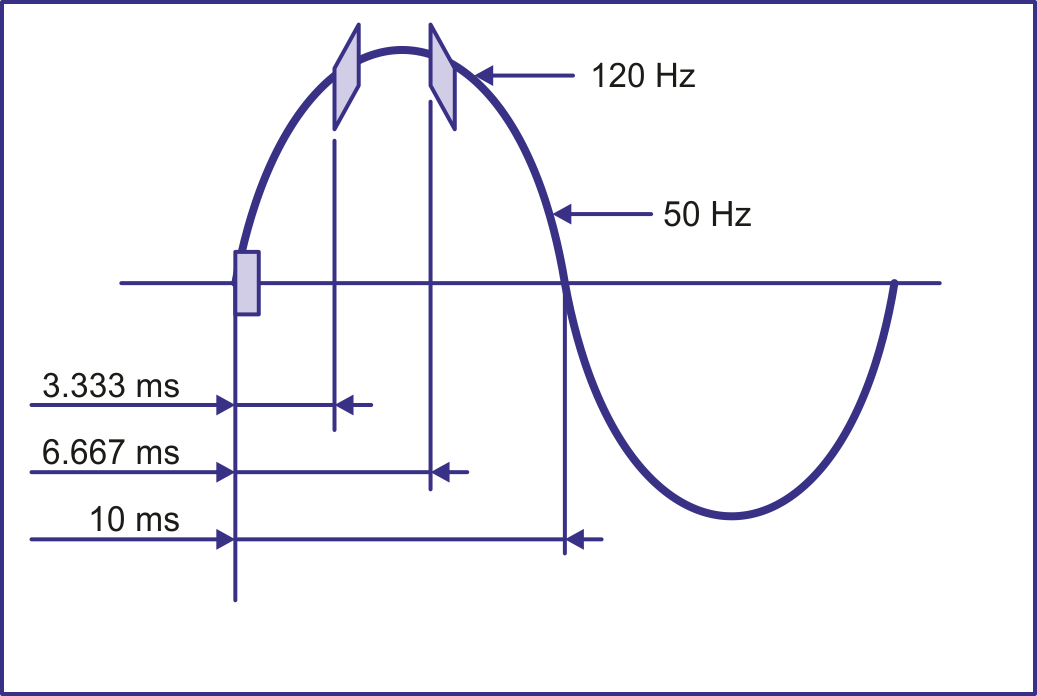
\includegraphics[width=0.8\textwidth]{imagenes/image_x10.png}
	\caption{Ejemplo de modulación de onda X-10}
	\label{fig:modulacionx10}
\end{figure}


La onda modulada actúa a lo largo de los ciclos como generadora de código digital. El protocolo X-10 se sirve de 11 ciclos de tensión alterna de 220 VAC, la misma de red, para insertar o no en cada ciclo la señal de 120 Khz. En general, la existencia de esta señal representa un uno y su ausencia un cero. Los primeros cuatro bits representan el código de inicio. Casi todos los protocolos tienen unos bits en su comienzo, que se utilizan para la sincronización y el alineamiento del transceptor, con un número codificado en binario que define al protocolo y lo mismo ocurre en el X-10.


La señal de 50 Hz (corriente) alimenta a los receptores y la señal de 120 Khz (de información) se filtra y es recibida por los receptores.


El protocolo X-10 usa una modulación muy sencilla comparada con las que usan otros protocolos de control por ondas portadoras. El transceptor X-10 est\'a pendiente de los pasos por cero de la onda senoidal de 50 Hz típica de la alimentación eléctrica (60 Hz en Estados Unidos) para insertar un instante después una r\'afaga muy corta de señal en una frecuencia fija.


Se puede insertar esta señal en los semiciclos positivos y negativos de la onda senoidal. La codificación de un bit uno o de un bit cero, depende de cómo se inyecte esta señal en los dos semiciclos. Un uno binario se representa por un pulso de 120 KHz durante uno ms y el cero binario se representa por la ausencia de ese pulso de 120 KHz. En un sistema trif\'asico el pulso de un ms se transmite tres veces para que coincida con el paso por el cero en cada una de las tres fases.


Por lo tanto, el Tiempo de bit coincide con los 20 ms que dura el ciclo de la señal, de forma que la velocidad binaria de 50 bps (bit/s) viene impuesta por la frecuencia de la red eléctrica que tenemos en Europa (50 Hz). En Estados Unidos la velocidad binaria son 60 bps (bit/s), ya que su frecuencia de la red eléctrica es de 60 Hz.


La transmisión completa de una orden X-10 necesita once ciclos de corriente. Esta trama se divide en tres campos de información:
\begin{enumerate}
	\item Dos ciclos representan el código de inicio.
	\item Cuatro ciclos representan el código de casa (letras A-P).
	\item Cinco ciclos representan o bien el código numérico (1-16) o bien el código de función (encender, apagar, aumento de intensidad, etc.)
\end{enumerate}


En la figura \ref{fig:trama_x10} se puede observar que inmediatamente después de los primeros dos ciclos que representan el código de inicio, cuatro bits, se tiene dos bloques: el primero representa el llamado código de casa y comprende otros cuatro bits y el segundo representa el llamado código de unidad y comprende los últimos cinco bits del protocolo.

\begin{figure}[htbp]
	\centering
		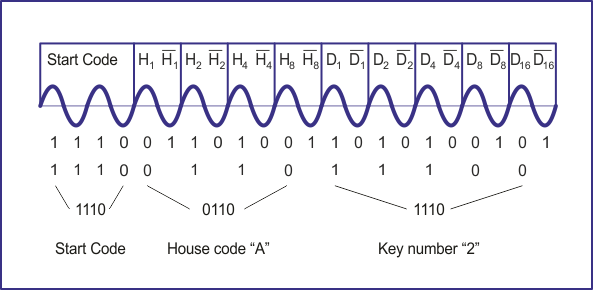
\includegraphics{imagenes/trama_x10.png}
	\caption{Trama de una petición en X-10}
	\label{fig:trama_x10}
\end{figure}


La forma de extraer la codificación en estos dos últimos bloques es ligeramente distinta a como se hace en el primero. Mientras en el código de inicio se toman en cuenta los semiciclos, en el código de casa y en el de unidad sólo se extrae la información del primer semiciclo de cada ciclo, aprovechando el segundo semiciclo para transmitir la señal del primero pero complementada. Esto se hace por seguridad. Así, en un ciclo de cualquiera de estos dos últimos bloques no puede haber dos ceros o dos unos seguidos, sí entre ciclos distintos.


Para aumentar la fiabilidad del sistema, esta trama (código de inicio, código de casa y código de función o numérico) se transmite siempre dos veces, separ\'andolas por tres ciclos completos de corriente. Hay una excepción, en funciones de regulación de intensidad se transmiten de forma continuada (por lo menos dos veces) sin separación entre tramas.


La nomenclatura Hn-Dn corresponde, respectivamente, al código de casa y al código de unidad y todas las combinaciones posibles se indican en la tabla \ref{tab:codigosx10}.

\begin{table}[htbp]
\centering
\begin{tabular}{cccccccccccc}
\toprule
\multicolumn{5}{c}{Códigos de casa} &  &\multicolumn{6}{c}{Códigos de unidad o dispositivo}\\ \toprule
  & H1 & H2 & H4 & H8 &    &    & D1 & D2 & D4 & D8 & D16\\ \midrule
A & 0  & 1  & 1  & 0  &    & 1  & 0  & 1  & 1  & 0  & 0\\
B & 1  & 1  & 1  & 0  &    & 2  & 1  & 1  & 1  & 0  & 0\\
C & 0  & 0  & 1  & 0  &    & 3  & 0  & 1  & 1  & 0  & 0\\
D & 1  & 0  & 1  & 0  &    & 4  & 1  & 0  & 1  & 0  & 0\\
E & 0  & 0  & 0  & 1  &    & 5  & 0  & 0  & 0  & 1  & 0\\
F & 1  & 0  & 0  & 1  &    & 6  & 1  & 0  & 0  & 1  & 0\\
G & 0  & 1  & 0  & 1  &    & 7  & 0  & 1  & 0  & 1  & 0\\
H & 1  & 1  & 0  & 1  &    & 8  & 1  & 1  & 0  & 1  & 0\\
I & 0  & 1  & 1  & 1  &    & 9  & 0  & 1  & 1  & 1  & 0\\
J & 1  & 1  & 1  & 1  &    & 10 & 1  & 1  & 1  & 1  & 0\\
K & 0  & 0  & 1  & 1  &    & 11 & 0  & 0  & 1  & 1  & 0\\
L & 1  & 0  & 1  & 1  &    & 12 & 1  & 0  & 1  & 1  & 0\\
M & 0  & 0  & 0  & 0  &    & 13 & 0  & 0  & 0  & 0  & 0\\
N & 1  & 0  & 0  & 0  &    & 14 & 1  & 0  & 0  & 0  & 0\\
O & 0  & 1  & 0  & 0  &    & 15 & 0  & 1  & 0  & 0  & 0\\
P & 1  & 1  & 0  & 0  &    & 16 & 1  & 1  & 0  & 0  & 0\\ \bottomrule \addlinespace
\multicolumn{12}{c}{Funciones}\\ \midrule
\multicolumn{7}{c}{Apagar todas las unidades} & 0 & 0 & 0 & 0 & 1 \\
\multicolumn{7}{c}{Encender todas las luces}  & 0 & 0 & 0 & 1 & 1 \\
\multicolumn{7}{c}{Encender}                  & 0 & 0 & 1 & 0 & 1 \\
\multicolumn{7}{c}{Apagar}                    & 0 & 0 & 1 & 1 & 1 \\
\multicolumn{7}{c}{Atenuar intensidad}        & 0 & 1 & 0 & 0 & 1 \\
\multicolumn{7}{c}{Aumentar intensidad}       & 0 & 1 & 0 & 1 & 1 \\ \bottomrule \addlinespace
\multicolumn{12}{c}{Códigos de función para controladores OEM}\\ \midrule 
\multicolumn{7}{c}{Apagar todas las luces}    & 0 & 1 & 1 & 0 & 1 \\
\multicolumn{7}{c}{Código extendido}          & 0 & 1 & 1 & 1 & 1 \\
\multicolumn{7}{c}{Petición de saludo}        & 1 & 0 & 0 & 0 & 1 \\
\multicolumn{7}{c}{Aceptación de saludo}      & 1 & 0 & 0 & 1 & 1 \\
\multicolumn{7}{c}{Atenuación preestablecida} & 1 & 0 & 1 & X & 1 \\
\multicolumn{7}{c}{Datos extendidos}          & 1 & 1 & 0 & 0 & 1 \\
\multicolumn{7}{c}{Estado = on}               & 1 & 1 & 0 & 1 & 1 \\
\multicolumn{7}{c}{Estado = off}              & 1 & 1 & 1 & 0 & 1 \\
\multicolumn{7}{c}{Petición de estado}        & 1 & 1 & 1 & 1 & 1 \\ \bottomrule
\end{tabular}
\caption{Códigos X-10}
\label{tab:codigosx10}
\end{table}




El sistema X-10 es de una topología flexible, tanto, que es posible sustituir elementos convencionales por dispositivos X-10 y un emisor puede activar los distintos receptores. En la figura \ref{fig:estructura_x10} se muestra un ejemplo de estructura de un sistema X-10:

\begin{figure}[htb]
	\centering
		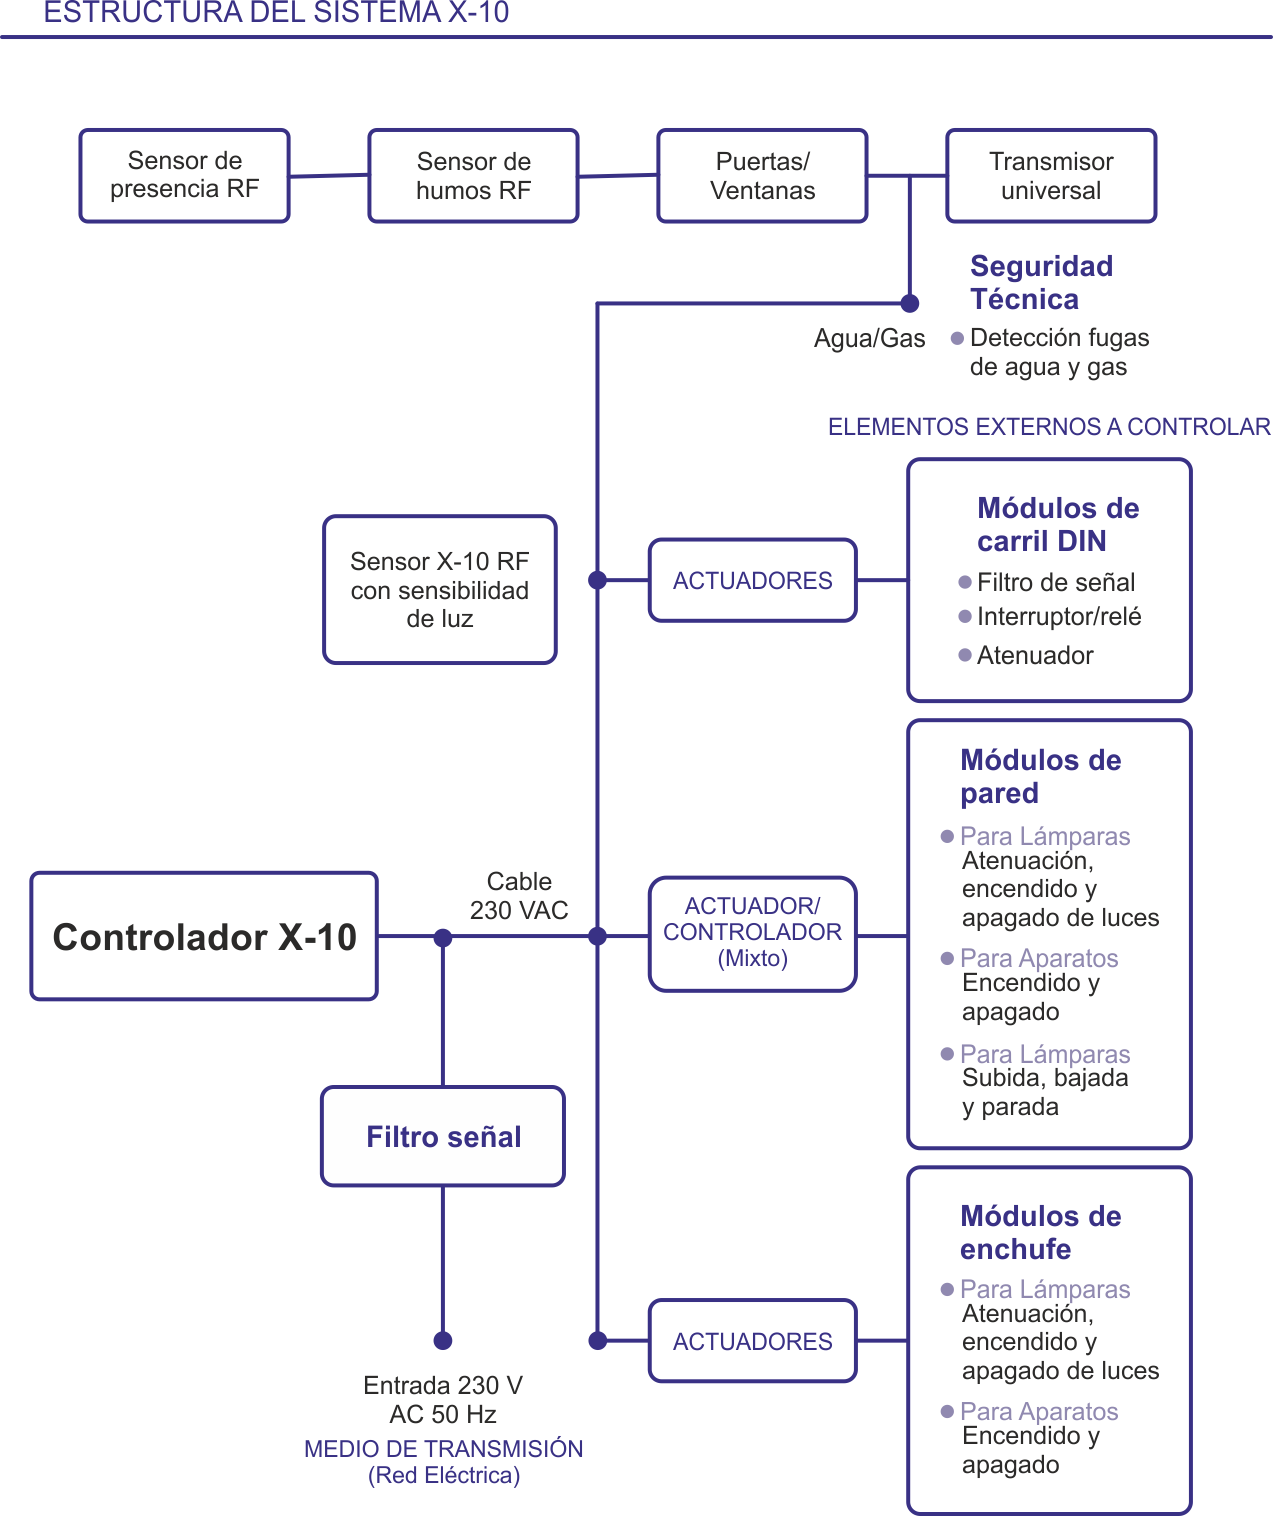
\includegraphics[width=0.8\textwidth]{imagenes/estructura_x10.png}
	\caption{Estructura de un sistema X-10}
	\label{fig:estructura_x10}
\end{figure}





Ademas el cambio de direccionamiento es sencillo ya que a todos los elementos se les puede cambiar su dirección física manipulando el propio dispositivo. Cada elemento lleva una o dos ruedas giratorias susceptibles de ser manipuladas con un simple destornillador, con lo que se puede determinar el código de casa y el código de unidad. Por ejemplo se podrían cofigurar dos o mas elementos con el mismo direccionamiento y activar los a la vez, en vez de activarlos uno a uno.


En conclusión, el protocolo X-10 es un sistema flexible, ampliable, de f\'acil instalación y económico. En su contra tiene la poca fiabilidad de sus comunicaciones, debido a que casi cualquier aparato eléctrico provoca interferencias en la línea eléctrica, y la baja velocidad de transmisión datos.
\clearpage
\subsection{LonWorks}
El protocolo LONWORKS, que también es conocido como LonTalk o el est\'andar de redes ANSI/EIA 709.1, es el corazón del sistema LONWORKS.


El protocolo provee de un conjunto de servicios de comunicación que permite al programa de aplicación de un dispositivo enviar y recibir mensajes de otros dispositivos sobre una red de control sin necesidad de conocer la topología de la red ni los nombres, direcciones o funciones de otros dispositivos. Los servicios de soporte para la gestión de la red permiten a las herramientas de gestión remota de la red interactuar con los dispositivos de la red, incluyendo:
\begin{itemize}
	\item Reconfiguración de las direcciones y par\'ametros.
	\item Descarga de programas de aplicación.
	\item Reporte de problemas de red.
	\item Arrancar, parar y/o resetear programas de aplicación de dispositivos
	\end{itemize}

El protocolo LONWORKS es un protocolo basado en paquetes caracterizado por la forma en la que se comunican los nodos entre si. Todo los nodos est\'an en igualdad de condiciones, de forma que no existe el concepto de cliente-servidor.



Adem\'as contempla una arquitectura de capas basada en el modelo OSI para asegurarse que cumple con los requerimientos específicos de un sistema de control de manera fiable y robusta.


El protocolo implementa las siete capas del modelo OSI:
\begin{figure}[htbp]
	\centering
		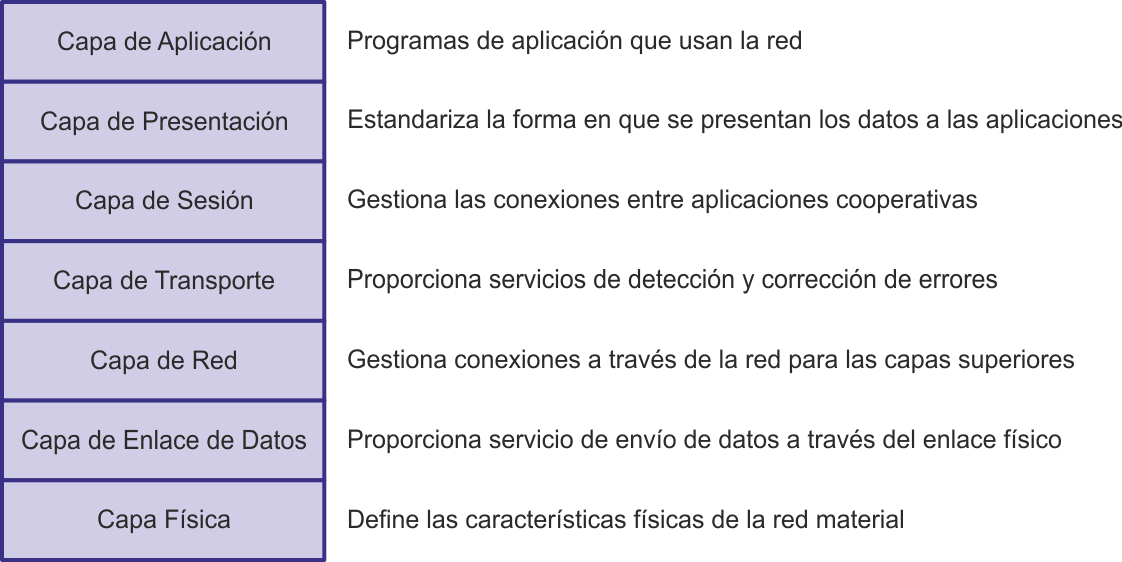
\includegraphics[width=0.80\textwidth]{imagenes/modelo_osi.png}
	\caption{Modelo OSI}
	\label{fig:modelo_osi}
\end{figure}



\begin{description}
	\item[Capa física] Se define el medio de transmisión. Este medio asegura que cada bit enviado por un dispositivo fuente es recibido a todos los dispositivos destino.
	
    \item[Capa de enlace]Define el método de acceso al medio y la codificación de datos para asegurar el uso eficiente del canal de comunicaciones. La capa de enlace define cu\'ando un dispositivo puede transmitir tramas de datos, cómo reciben los dispositivos dichas tramas y detecta errores en la transmisión.
	
    \item[Capa de red]Define cómo se mandan los paquetes de mensaje desde un dispositivo fuente a uno o m\'as dispositivos destino. En esta capa se define la manera de nombrar y direccionar los dispositivos de manera que asegure la correcta entrega de paquetes, adem\'as de definir cómo se realiza el ruteado de los mensajes en los diferentes canales de comunicación.
	
    \item[Capa de transporte]Asegura una entrega fiable de paquetes. Los mensajes pueden ser intercambiados usando un servicio de reconocimiento, de manera que el dispositivo emisor, esperar\'a a recibir un “reconocimiento” del receptor y reenviar el mensaje si el reconocimiento no es recibido. En esta capa también se define cómo detectar mensajes duplicados y cómo son rechazados si un mensaje es reenviado por falta de reconocimiento ‘acknowledgement’.
    
	\item[Capa de sesión]Añade control al intercambio de datos entre las capas inferiores. Soporta las acciones remotas para que un cliente pueda enviar peticiones a un servidor remoto y recibir la respuesta a esta petición.También chequea la autorización de los dispositivos emisores. 
    	
    \item[Capa de presentación]Añade una estructura a los datos intercambiados entre las capas inferiores definiendo la codificación de los datos de mensaje. Los mensajes pueden ser codificados como variables de red, mensajes de aplicación, o tramas externas. La codificación interoperable de las variables de red se consigue con el est\'andar de los tipos de variables de red (SNVTs).
	
    \item[Capa de aplicación]aporta compatibilidad de aplicaciones a los datos intercambiados por las otras capas. Esta capa también define un protocolo de transferencia que es usado para transferir cadenas de datos entre las distintas aplicaciones.
\end{description}

Todas las comunicaciones consisten en el intercambio de uno o m\'as paquetes entre dispositivos. Cada paquete es un número variable de bytes y contiene una representación de los datos requeridos para cada una de las siete capas. En LONWORKS, esta representación de paquetes es muy corta, minimizando el coste de la implementación de cada dispositivo.


Para poder comunicar, cada dispositivo conectado a un canal, estar\'a siempre observando los paquetes sobre el canal para ver si alguno lleva su dirección. En caso afirmativo, mirar\'a si es un paquete de datos para su aplicación o si es un paquete de gestión. En caso de que fuera un paquete de datos de aplicación, estos datos son transferidos al programa de aplicación y en caso de que sea necesario, se responder\'a al dispositivo emisor con un mensaje de autenticación o reconocimiento.


Hasta hace muy pocos años, el protocolo LONWORKS estaba solo disponible embebido en el ‘Neuron Chip’. Esto aseguraba una aplicación consistente para todos los fabricantes. Ahora que hay un gran número de dispositivos compatibles instalados, Echelon Corporation ha publicado el protocolo LONWORKS y lo ha convertido en un est\'andar abierto dentro de la ANSI/EIA709.1 Est\'andar de Redes de Control. El protocolo es, por tanto, de libre disposición para todo el mundo. Aun así, la manera m\'as económica y efectiva de implementar este protocolo sigue siendo con la utilización del Neuron Chip.

Este Neuron Chip fue creado por Echelon, el nombre le fue puesto para hacer una similitud con el cerebro humano, ya que esta formado por neuronas que, a diferencia de un control 
centralizado, reparten el control en millones de ellas,estando interconectadas y cada una proveyendo información por múltiples rutas. Cada una de ellas suele estar dedicada a una función específica, pero la pérdida de una de ellas no implica la pérdida de funcionalidad del sistema. El ‘Neuron Chip’ incluye las primeras 6 capas del modelo OSI/ISO, por lo que el desarrollador sólo tiene que preocuparse del programa de aplicación. Es un dispositivo semiconductor especialmente diseñado para proveer inteligencia y capacidades de comunicación a dispositivos de control de bajo coste. Incluye 3 procesadores, 2 para comunicación y 1 para el procesamiento de la aplicación. Los fabricantes de dispositivos proveen el código de aplicación que corre en el‘Neuron Chip’ y los dispositivos de E/S para ser conectados al el.


El Neuron Chip tiene en su interior una memoria ROM que contiene un sistema operativo completo, llamado ‘Neuron Chip Firmware’, incluyendo el protocolo LONWORKS y una librería de funciones de E/S (Entrada/Salida). El chip tiene una memoria no vol\'atil para los datos de configuración y para el programa de aplicación.


Cada dispositivo LONWORKS unido a la red, normalmente contiene un ‘Neuron Chip’ y un transceptor. Dependiendo de la función del dispositivo, puede haber también sensores y actuadores embebidos e interfaces de entrada y salida a sensores y actuadores. El programa de aplicación que es ejecutado por el ‘Neuron Chip’ puede residir permanentemente en una ROM o puede ser descargado sobre la red en una memoria no vol\'atil de lectura/escritura (NVRAM, flash PROM, o EEPROM).


El trabajo de la mayor parte de los dispositivos en una red LONWORKS es sensorizar y controlar el estado de los componentes que forman el sistema físico. Estos son llamados dispositivos de control LONWORKS.


El programa de aplicación de un dispositivo, puede enviar y recibir valores dela red, realizar procesamiento de los datos (linearización, escalado,…) de las variables sensorizadas y procesar datos de lógicas de control como lazos de control PIDs.

\subsection{KNX}
La asociación KNX o Konnex nace en 1999 como la iniciativa de tres organizaciones, que ya llevaban años en el mercado europeo, aunque con tecnologías bien diferentes, así como objetivos y \'ambitos de actuación complementarios. Estas organizaciones son: EIBA, BatiBUS y EHS.


En la actualidad, la organización que m\'as ha realizado para conseguir un protocolo común ha sido EIB, por lo que el protocolo es también conocido como KNX-EIB. A día de hoy, KNX es el único protocolo certificado libre que existe especializado en la domótica.


Los medios de comunicación que usa el protocolo KNX son los siguientes: 
\begin{itemize}
	\item Par trenzado (TP1): aprovechando la norma EIB equivalente.
	\item Par trenzado (TP0): aprovechando la norma Batibus equivalente. 
	\item Ondas Portadoras (PL100): aprovechando la norma EIB equivalente.
	\item Ondas Portadoras (PL132): aprovechando la norma EHS equivalente. 
	\item Ethernet: aprovechando la norma EIB.net. 
	\item Radiofrecuencia: aprovechando la norma EIB.RF
\end{itemize}
La elección de un medio de transmisión u otro depender\'a del tipo de edificio y de las instalaciones con las que éste cuente. Así, si el edificio es de nueva construcción el par trenzado es quiz\'as el medio m\'as óptimo, mientras que si el edificio est\'a ya construido es posible que interese m\'as el uso de la línea de potencia o radiofrecuencias.


En el sistema KNX la transmisión de las señales se hace a través de un cable o bus al que est\'an conectados todos los dispositivos. El bus permite que todos los componentes de las instalaciones domóticas estén intercomunicados entre sí, de esta forma, es posible que cualquier componente de órdenes a cualquier otro, independientemente de la distancia entre ellos y su ubicación. 


La unidad de instalación mas pequeña la forma la línea. Una línea consta de un m\'aximo de cuatro segmentos de línea, cada uno de los cuales puede disponer de 64 componentes del bus (256 elementos por linea). Mediante el uso de acopladores de línea es posible unir hasta 15 lineas en una zona (3840 elementos por zona). Cada línea dispondr\'a de su fuente de alimentación EIB, y estar\'a separada galv\'anicamente del resto de líneas. Esto es importante, porque supone que si se produce un fallo en alguna línea, el resto seguir\'a funcionando normalmente. También se pueden usar acopladores de zona, para unir distintas zonas a través de una línea principal, hasta un m\'aximo de 15. Con lo cual, podemos tener hasta 57600 elementos en total.

La división en zonas y líneas es muy ventajosa, ya que significa que el trafico de información local , no afecta a los datos del resto de líneas o zonas. El acoplador de línea impedir\'a el paso hacia otras líneas de datagramas cuyos destinos sena elementos de su línea. Y, al mismo tiempo ignorara aquellos datagramas provenientes de otras líneas o zonas que no conciernan a elementos de su línea. Esto posibilitara la comunicación simultanea en múltiples líneas independientes unas de otras y sin congestionar la red.


Gracias a la división jerarquica en zonas y líneas, la instalación de un sistema EIB resulta f\'acilmente comprensible a la hora de la puesta en marcha, el diagnostico y las tareas de mantenimiento. Comenzando por unas pocas líneas al principio de la instalación, es posible ampliar paso a paso el sistema cuando y como las nuevas necesidades o usos de las instalaciones así lo requieran.


En la figura \ref{fig:estructuraknx} podemos ver un ejemplo de conexión de líneas y \'areas:

\begin{figure}[ht]
	\centering
		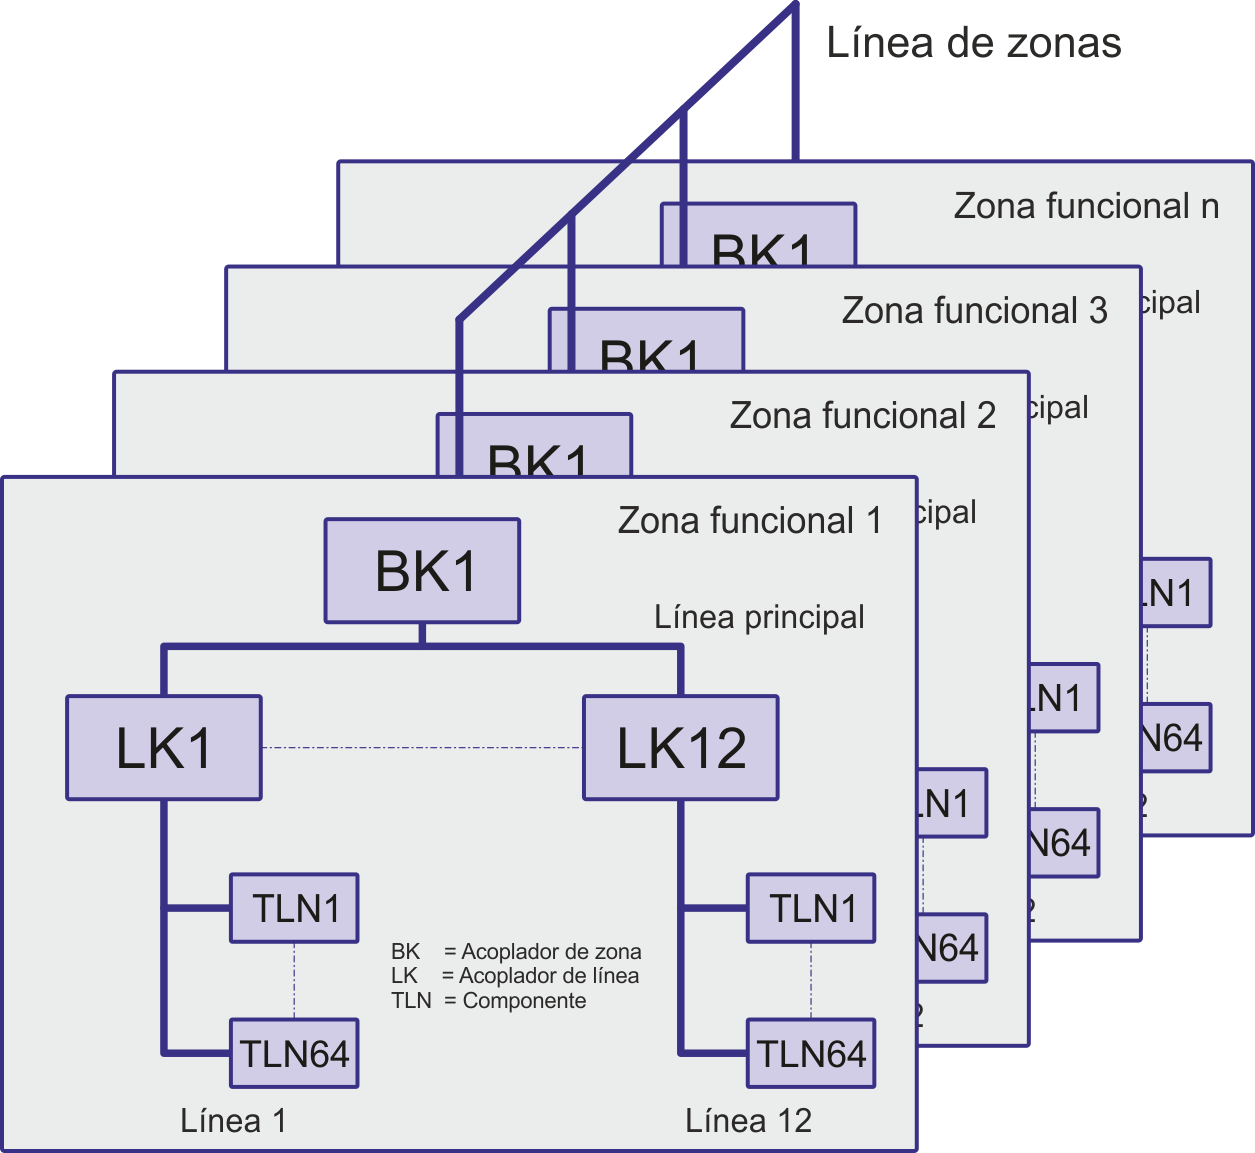
\includegraphics[width=0.8\textwidth]{imagenes/Acopladores-Knx.png}
	\caption{Estructura KNX}
	\label{fig:estructuraknx}
\end{figure}


Una vez visto cómo se estructura, vamos a ver cómo se envían los datos el protocolo KNX. La información que circula por el bus, como por ejemplo las ordenes de conmutación, es intercambiada entre los componentes conectados al bus en forma de datagramas o telegramas. La información se transmite de forma simétrica en el bus, es decir, como una diferencia de potencial entre los dos hilos y no referida a tierra, como muestra la figura \ref{fig:transmisionknx}. De esta forma, las interferencias o ruido, al afectar a ambos hilos de forma similar, influyen en menor grado en la transmisión de la información. 


\begin{figure}[ht]
	\centering
		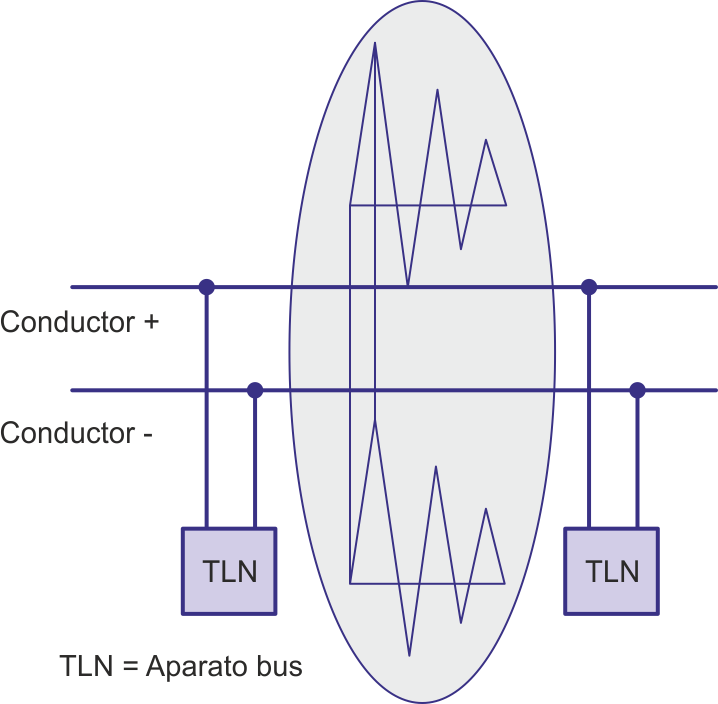
\includegraphics[width=0.8\textwidth]{imagenes/topologia-knx.png}
	\caption{Transmisión de la señal KNX}
	\label{fig:transmisionknx}
\end{figure}



La tasa de transmisión es de 9600 bit/s, siendo el tiempo medio de transmisión de un datagrama de unos 25 ms.


Para enviar un telegrama, lo primero que hace un dispositivo es esperar un tiempo hasta que el medio por el que va a transmitir esté libre, y una vez que esté libre espera un tiempo también para comprobar que nadie ha empezado a enviar datos. Si esto se cumple, empezaría con la transmisión y una vez terminado este envío, se espera un tiempo hasta que los dispositivos a los que se les ha enviado la información confirmen que han recibido bien el paquete. 



Aparte, cada byte de datos se agrupan formando caracteres o palabras, que adem\'as de estos datos se componen de otros bits como se puede observar en la figura \ref{fig:palabra_knx}.
\begin{figure}[htbp]
	\centering
		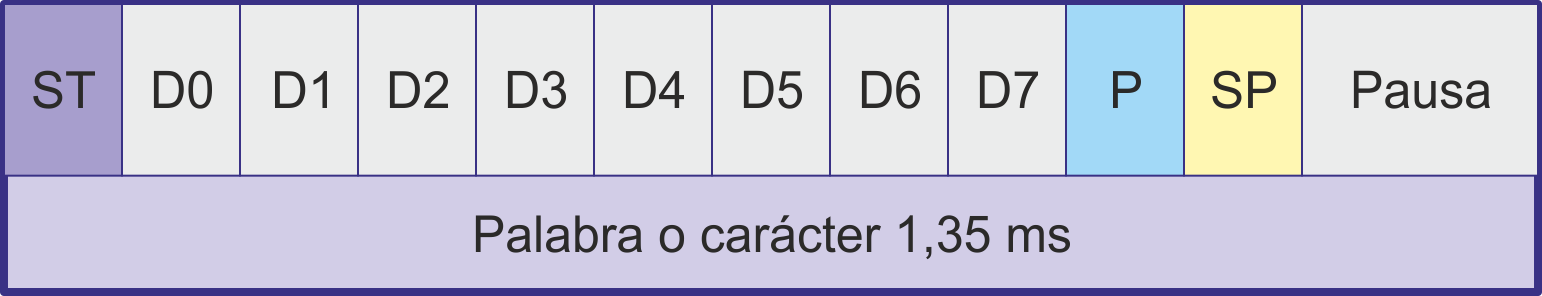
\includegraphics[width=0.80\textwidth]{imagenes/palabra_knx.png}
	\caption{Bits de una palabra en KNX}
	\label{fig:palabra_knx}
\end{figure}


\begin{description}
	\item[ST]Es un bit de inicio, que indica el comienzo de una nueva palabra.
	\item[P]Es el llamado bit de paridad, trabaja con paridad par y completa la suma de los bits de datos, para trabajar con dicha paridad.
	\item[SP]Es un bit de parada, e indica que la palabra o carácter ha terminado.
	\item[Pausa]Después del bit de parada se espera un tiempo de pausa equivalente a dos bits para continuar con la próxima palabra.
\end{description}

Estos caracteres van dentro de un paquete de datos, que está formado por los campos mostrados en la figura\ref{fig:campos_paq_knx}.
\begin{figure}
	\centering
		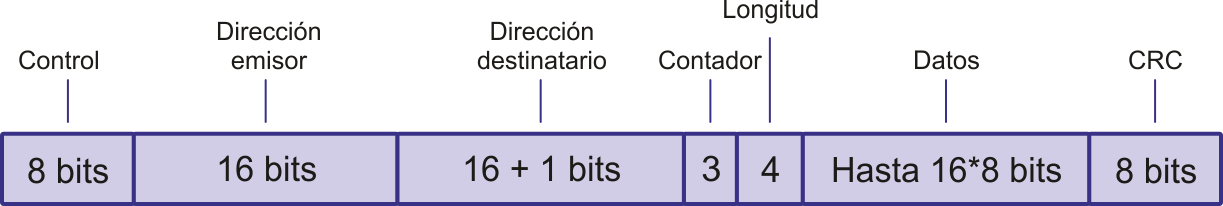
\includegraphics[width=0.80\textwidth]{imagenes/campos_paq_knx.png}
	\caption{Campos de un paquete KNX}
	\label{fig:campos_paq_knx}
\end{figure}


El byte de control indica la prioridad del mensaje y el inicio del mismo. Tanto la dirección del emisor como la del destinatario siguen un formato determinado, añadiendo un bit más en la dirección del destinatario que indica si se trata de una dirección física o de una dirección de grupo. El contador se utiliza para funciones de enrutamiento, contando el número de saltos que ha dado el paquete. El último byte, CRC, se utiliza para comprobar que los anteriores han sido transmitidos correctamente.


La dirección física se utiliza para identificar de manera unívoca el componente de bus, describiendo su localización dentro de la topología (zona, línea y componente) dedicando los cuatro primeros bits a la zona (15 zonas), los cuatro siguientes a la línea (15 líneas) y los ocho últimos a los componentes (256 componentes).


En caso de que esta dirección sea de grupo, la forma de crearla es diferente, y se puede hacer con dos o tres subgrupos. Los subgrupos pueden ser, por ejemplo, los siguientes:
\begin{description}
	\item[Grupos principales] bombillas, persianas, aire acondicionado…
	\item[Grupo intermedio] primera planta, segunda planta…
	\item[Grupo secundario] oficinas, dormitorio…
\end{description}


Para ello destinamos 4 bits al grupo principal y dependiendo de si tenemos grupo intermedio o no, 3 bits para el intermedio y 8 para el secundario o directamente 11 para el secundario. El último bit es para indicar si la dirección era de grupo o dirección física. Esto se ve mejor en la figura \ref{fig:Niveles-direccionamiento-grupo-knx}.
\begin{figure}[htbp]
	\centering
		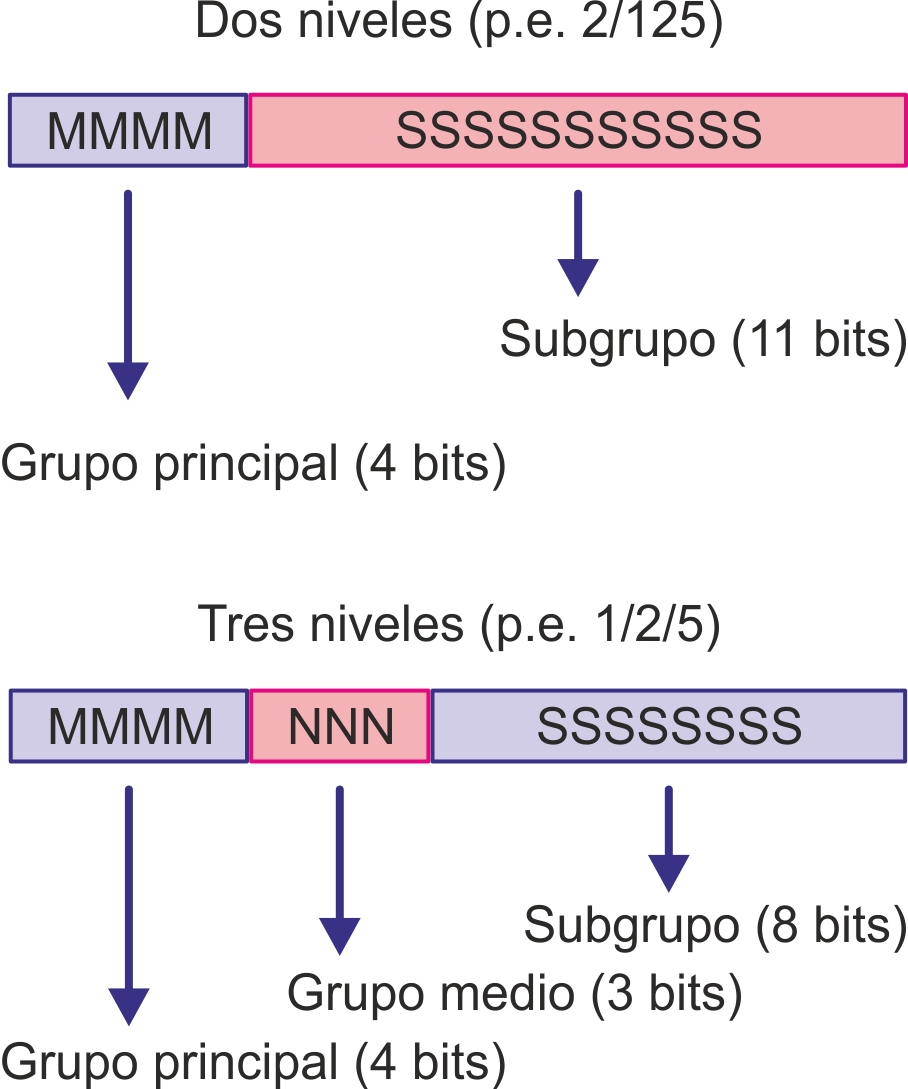
\includegraphics[height=0.70\textwidth]{imagenes/Niveles-direccionamiento-grupo-knx.png}
	\caption{Direccionamiento en KNX}
	\label{fig:Niveles-direccionamiento-grupo-knx}
\end{figure}



Las direcciones de grupo son básicas para el funcionamiento del sistema ya que permiten relacionar sensores con actuadores. Además, estará permitido relacionar elementos de distintas áreas y distintas líneas, siempre y cuando se cumplan ciertas restricciones:
\begin{itemize}
	\item Los sensores sólo pueden tener asociada una dirección de grupo.
	\item Varios actuadores pueden tener asociada una misma dirección de grupo. Cada vez que dicha dirección sea direccionada, se activarán todos los actuadores asociados a ella, respondiendo todos ellos al mismo telegrama.
	\item Los actuadores pueden estar asociados a varias direcciones de grupos, es decir, un actuador puede estar asociado a uno o más de un sensor.
\end{itemize}


El funcionamiento será el siguiente: el emisor envía un telegrama al bus. Este telegrama llega a todos los dispositivos, lo cuales leen el campo dirección de grupo y sólo los que posean dicha dirección responden de la forma oportuna.


Una vez los dispositivos se pueden interconectar, sólo hace falta que se entiendan entre ellos. Para ello, es preciso que se comuniquen en el mismo “lenguaje”. Existen diferentes tipos de variables para transmitir los datos y están todas definidas dentro del EIS (EIB Interworking Standard). En la tabla \ref{tab:variables_eib} podemos ver un fragmento del mismo con las variables más usadas.

\begin{table}[htbp]
\centering \scriptsize
%\resizebox{\textwidth}{!} {
\begin{tabular}{cp{4cm}cp{5.5cm}}
\multicolumn{4}{c}{EIS (EIB Interworking Standard)} \\ \toprule
Nº EIS& Función EIB              & Nº de Bytes &  Descripción \\ \midrule
EIS 1 & interruptor (switching)  & 1 bit & encendido/apagado, verdadero\/falso \\ \midrule
EIS 2 & regulación (dimming)     & 4 bit & Se puede utilizar de 3 formas distintas:  como interruptor, como valor relativo  y como valor absoluto. \\ \midrule
EIS 3 & hora (time)              & 3 bytes    & día de la semana, hora, minutos y segundos. \\ \midrule
EIS 4 & fecha (date)             & 3 bytes   & Día\/mes\/año (el margen es de 1990 a 2089). \\ \midrule
EIS 5 & valor (value)            & 2 bytes  & Para enviar valores físicos con representación  S,EEEE,MMMMMMMMMMM \\ \midrule
EIS 6 & escala (scaling) & 8 bit & Se utiliza para transmitir valores relativos  con una resolución de 8 bit. Ej. FF = 100\% \\ \midrule
EIS 7 & control motores (control drive) & 1 bit & Tiene dos usos: \ Mover, arriba\/abajo o extender\/retraer y Paso a Paso. \\ \midrule
EIS 8 & prioridad (priority) & 1 bit & Se utiliza en conjunción con EIS 1 ó EIS 7. \\ \midrule
EIS 9 & coma flotante (float value) & 4 bytes & Codifica un número en coma flotante  según el formato definido por el IEEE 754. \\ \midrule
EIS 10 & contador 16 bit (16b-counter) & 2 bytes & Representa los valores de un contador de 16 bit  (tanto con signo como sin signo). \\ \midrule
EIS 11 & contador 32 bit (32b-counter) & 4 bytes & Representa los valores de un contador de 32 bit  (tanto con signo como sin signo). \\ \midrule
EIS 12 & acceso (access) & 4 bytes & Se usa para conceder accesos a distintas funciones. \\ \midrule
EIS 13 & Carácter ASCII (Character) & 8 bit & Codifica según el formato ASCII \\ \midrule
EIS 14 & contador 8 bit (8b-counter) & 8 bit & Representa los valores de un contador de 8 bit  (tanto con signo como sin signo). \\ \midrule
EIS 15 & Cadena (Character String) & 14 bytes & Transmite una cadena de caracteres ASCII  de hasta 14 bytes. \\ \bottomrule
\end{tabular}
%}
\caption{Variables mas usadas en EIB}
\label{tab:variables_eib}
\end{table}




	\chapter{Redes de sensores: Estado del arte}

En el estudio de los distintos sistemas domoticos vemos que estos realmente solo son una red de sensores y actuadores con un enfoque muy concreto, la vivienda. Por ello veamos con mas detenimiento las redes de sensores, en especial las redes inal\'ambricas.

La idea de una red de sensores surge gracias a las posibilidades que nos da la tecnolog\'ia de crear una red de
dispositivos de captura constante, que nos permita registrar y almacenar una determinada informaci\'on, transmitir datos de un dispositivo a otro, y despu\'es retransmitir toda la informaci\'on para almacenarla en una localizaci\'on central.

Las redes de sensores con cable no son nuevas y sus funciones han sido, tradicionalmente, medir niveles de temperatura, l\'iquido, humedad etc. La diferencia entre estos sensores que todos conocemos y la nueva generaci\'on de WSN es que estos \'ultimos son inteligentes, capaces de poner en marcha una acci\'on seg\'un la informaci\'on que vayan acumulando y, adem\'as, no est\'an limitados por su conexi\'on a trav\'es de un cable e incluso puede ser m\'oviles. 

Los nuevos avances en la fabricaci\'on de microchips, los nuevos est\'andares de comunicaciones inal\'ambricas, las nuevas funcionalidades de routers y equipamientos de red, los nuevos desarrollos de software y programas inform\'aticos est\'an logrando eliminar los cables de las redes de sensores, multiplicando as\'i su potencial.

\section{Redes inal\'ambricas de sensores} 

Una red de sensores (o WSN, Wireless Sensor Network, en ingl\'es) es una red de dispositivos, equipados con sensores, y de comunicaci\'on inal\'ambrica que permiten formar redes ad-hoc sin infraestructura f\'isica preestablecida ni administraci\'on central.


La expresi\'on ad-hoc hace referencia a una red en la que no hay un nodo central, sino que todos los dispositivos est\'an en igualdad de condiciones. Ad-hoc es el modo m\'as sencillo para crear una red, un tipo de red formada por un grupo de nodos que forman una red temporal sin la ayuda de ninguna infraestructura externa. Para que esto se pueda llevar a la pr\'actica es necesario que los nodos se puedan ayudar mutuamente para conseguir un objetivo com\'un: que cualquier paquete llegue a su destino aunque el destinatario no sea accesible directamente desde el origen.


El protocolo de encaminamiento es el responsable de descubrir las rutas entre los nodos para hacer posible la
comunicaci\'on. Las redes de sensores son un concepto relativamente nuevo en adquisici\'on y tratamiento de datos con m\'ultiples aplicaciones en distintos campos, tales como entornos industriales, dom\'otica, entornos militares, detecci\'on ambiental. Esta clase de redes se caracterizan por su facilidad de despliegue y por ser autoconfigurables, pudiendo convertirse en todo momento en emisor, receptor, ofrecer servicios de encaminamiento entre nodos sin visi\'on directa, as\'i como registrar datos referentes a los sensores locales de cada nodo.


Las redes de sensores es un tema muy activo de investigaci\'on en varias universidades, aunque ya empiezan a existir aplicaciones comerciales basadas en este tipo de redes. 


La lista de aplicaciones donde las WSN encuentran utilidad puede ser ingente y abierta a la creatividad. Los usos m\'as t\'ipicos est\'an relacionados con tareas de supervisi\'on, seguimiento y control. 



Algunos de los usos espec\'ificos son:

\begin{itemize}
\item Dom\'otica.
\item Control/Supervisi\'on del medio ambiente.
\item Detecci\'on ac\'ustica.
\item Detecci\'on s\'ismica.
\item Detecci\'on/Control actividad nuclear.
\item Vigilancia militar.
\item Seguimiento de inventario.
\item Seguimiento de objetos, personas.
\item Supervisi\'on m\'edica.
\item Espacios inteligentes.
\item Control de procesos operativos.
\item Gesti\'on tr\'afico en ciudades y carreteras.
\end{itemize}

 

\section{Arquitectura del sistema}

Las redes de sensores est\'an formadas por un conjunto de peque\~nos dispositivos con capacidad limitada de c\'omputo y  comunicaci\'on, cuyo tiempo de vida depende de una bater\'ia adjunta al dispositivo. El tiempo de vida de la red de sensores depender\'a por tanto del tiempo de vida de la bater\'ia de sus nodos.

Estos dispositivos se encuentran dispersos de manera ad-hoc en una determinada \'area a monitorizar. En redes de comunicaci\'on, dicha expresi\'on hace referencia a una red en la que no hay un nodo central, sino que todos los nodos est\'an en igualdad de condiciones.

T\'ipicamente, el modelo seguido por las aplicaciones es el siguiente: realizar una serie de mediciones sobre el medio, transformar dicha informaci\'on en digital en el propio nodo y transmitirla fuera de la red de sensores v\'ia un elemento gateway a una estaci\'on base, donde la informaci\'on pueda ser almacenada y tratada temporalmente para acabar finalmente en un servidor con mayor capacidad que permita componer un hist\'orico o realizar an\'alisis de datos, por lo tanto, podemos encontrarnos: 

\begin{itemize}
\item nodos inal\'ambricos 
\item puertas de enlace 
\item estaciones base
\end{itemize}

\begin{figure}[htbp]
	\centering
		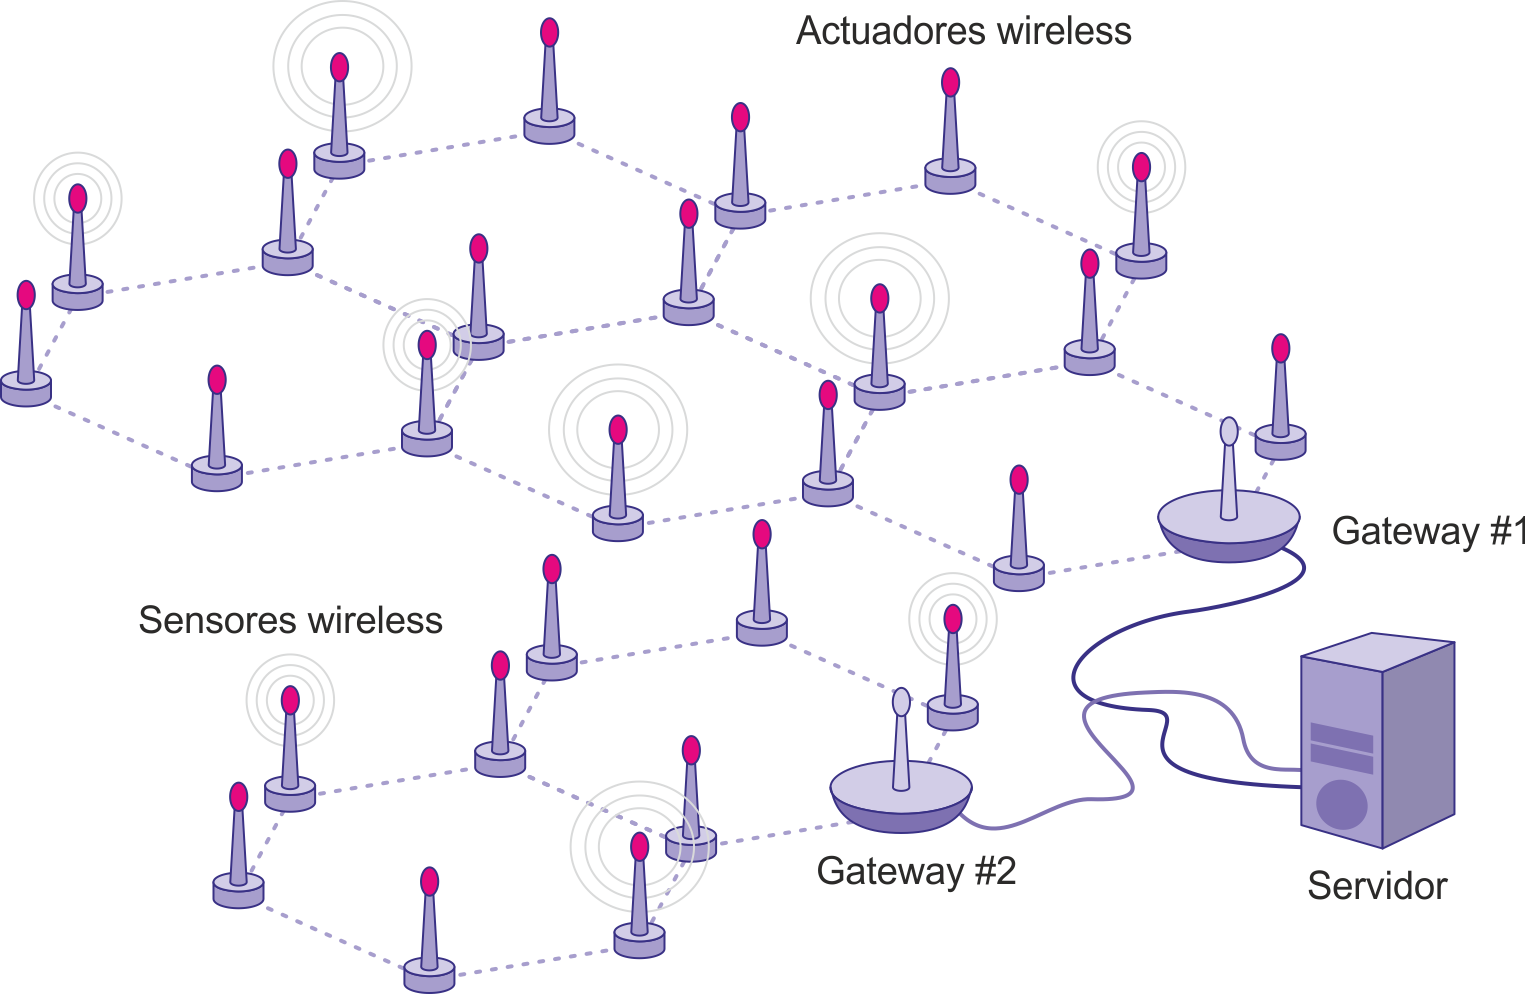
\includegraphics[width=0.8\textwidth]{imagenes/red_de_sensores.png}
	\caption{Red de sensores}
	\label{fig:red_de_sensores}
\end{figure}

 

\subsection{Nodo inal\'ambrico}
Los nodos inal\'ambrico son dispositivos electr\'onicos capaces de captar informaci\'on proveniente del entorno en el que se encuentran, procesarla y transmitirla inal\'ambricamente hacia otro destinatario. 

El tama\~no de un nodo puede variar desde una caja de zapatos hasta un grano de polvo. El coste de estos nodos es igualmente variable, extendi\'endose desde centenas de euros a algunos c\'entimos, dependiendo del tama\~no de la red del sensor y de la complejidad requerida de cada nodo individual. Las limitaciones de tama\~no y de coste en el nodo del sensor dan lugar a restricciones en recursos tales como energ\'ia, memoria, velocidad de proceso y anchura de banda.

El hardware de cada uno de estos dispositivos tiene varias partes bien diferenciadas como se puede ver en la figura \ref{fig:partes_nodo}.

\begin{figure}[htbp]
	\centering
		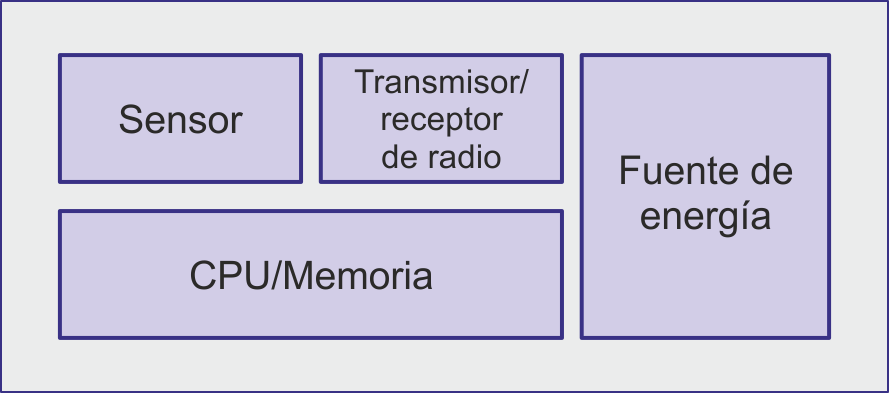
\includegraphics[width=0.8\textwidth]{imagenes/partes_nodo.png}
	\caption{Partes de un nodo}
	\label{fig:partes_nodo}
\end{figure}

 


\subsubsection{Procesador}
Es el componente que interpreta y procesa los datos para transmitirlos a otra estaci\'on. Tambi\'en gestiona el
almacenamiento de datos en la memoria. Puesto que de un nodo sensor se espera una comunicaci\'on y una recogida de datos mediante sensores, debe existir una unidad de procesado, que se encargue de gestionar todas estas operaciones. 

Hay muchos tipos diferentes de productos disponibles en el mercado para ser integrados en un nodo, como
microcontroladores, microprocesadores y FPGA. 

\begin{description}
	\item[FPGA]
	Actualmente \'estas presentan varias desventajas, la mayor de ellas es el consumo. A pesar de que en el mercado podemos encontrar FPGAs de bajo consumo, este consumo no es lo suficientemente bajo como deber\'ia ser para este tipo de nodos. Esto no significa que en un futuro cercano, \'estas sean una buena opci\'on si se consigue que reduzcan el consumo.
	\item[Microprocesadores]
	Han sido sustituidos por los microcontroladores, ya que \'estos integran dentro de un mismo dispositivo, un microprocesador y memoria.
	\item[Microcontroladores]
	Como se ha dicho, incluyen un microprocesador y memoria, pero adem\'as tienen una interface para ADCs, UART, SPI, temporizadores y contadores. Hay muchos tipos de microcontroladores que van desde los 4 bits hasta 64 bits, con una variaci\'on del numero de temporizadores, con diferentes consumos de energ\'ia, etc...
\end{description}
 

Algunos de los m\'as utilizados son los siguientes procesadores de bajo consumo:

\begin{itemize}
\item ARM7
\item Atmel AVR
\item Intel Xscale
\item PIC
\end{itemize}


\subsubsection{Alimentaci\'on}
Normalmente la fuente de alimentaci\'on son bater\'ias dif\'icilmente sustituibles o transformadores con salida adecuada para el nodo si se dispone de toma de corriente. Para las situaciones en donde no se dispone de red el\'ectrica y las posibilidad de sustituir las bater\'ias es muy complicada, se est\'an estudiando diferentes t\'ecnicas para alimentar el sensor, como puede ser mediante placas solares. 

Ante la limitaci\'on de la vida \'util del dispositivo hay que realizar una gesti\'on eficiente del consumo energ\'etico. El consumo de energ\'ia viene dado por lo que consumen los sensores, la comunicaci\'on y el procesado. La mayor cantidad de energ\'ia es consumida en la transmisi\'on de informaci\'on, siendo menor en el procesado y uso de los sensores.

\ Las bater\'ias son la principal fuente de energ\'ia de los nodos, pudiendo ser recargables o no recargables. Actualmente se est\'an estudiando sistemas basados en energ\'ia renovables para solucionar el problema de la energ\'ia en estos nodos, basados en energ\'ia solar, termo generaci\'on, energ\'ia basada en vibraciones, etc...

\subsubsection{Comunicaci\'on Inal\'ambrica }
El dispositivo de comunicaci\'on se trata de un dispositivo v\'ia radio que permite enviar y recibir datos para comunicarse con otros dispositivos dentro de su rango de transmisi\'on. 

Los nodos usan la banda ISM que son bandas reservadas internacionalmente para uso no comercial de radiofrecuencia electromagn\'etica en \'areas industrial, cient\'ifica y m\'edica. El uso de estas bandas de frecuencia est\'a abierto a todo el mundo sin necesidad de licencia, respetando las regulaciones que limitan los niveles de potencia transmitida. Los medios a elegir para realizar una comunicaci\'on inal\'ambrica son varios, radio frecuencia, comunicaci\'on \'optica mediante l\'aser e infrarrojos. 

La comunicaci\'on por l\'aser es la que menos energ\'ia consume pero requiere de una comunicaci\'on visual entre emisor y receptor, y adem\'as tambi\'en depende de las condiciones atmosf\'ericas. 

Los infrarrojos como el l\'aser, no necesitan antena, aunque es bastante limitado en su capacidad de transmisi\'on. 

La radio frecuencia, RF, es la m\'as adecuada para usar en aplicaciones inal\'ambricas. Las WSN usan las frecuencias de comunicaci\'on que andan entre 433 MHz y 2.4 Ghz.

\subsubsection{Sensores}
Los sensores son dispositivos hardware que producen una respuesta medible ante un cambio en un estado f\'isico, como puede ser temperatura o presi\'on. Los sensores detectan o miden cambios f\'isicos en el \'area que est\'an monitorizando. La se\~nal anal\'ogica continua detectada es digitalizada por un convertidor anal\'ogico digital y enviada a un controlador para ser procesada.

Las caracter\'isticas y requerimientos que un sensor debe tener son un peque\~no tama\~no, un consumo bajo de energ\'ia, operar en densidades volum\'etricas altas, ser aut\'onomo y funcionar desatendidamente y tener capacidad para adaptarse al ambiente. 

Los sensores pueden estar clasificados en tres categor\'ias: 

\begin{description}
\item [Sensores pasivos omnidireccionales]
 Los sensores pasivos captan los datos sin necesidad de manipular el entorno. Son autoalimentados y solo usan la energ\'ia para amplificar la se\~nal anal\'ogica captada. No hay ninguna noci\'on de direcci\'on involucrada en estas mediciones.

\item [Sensores pasivos unidireccionales] 
Son sensores pasivos que tienen bien definida la direcci\'on desde donde deben captar la informaci\'on. Un ejemplo t\'ipico es una c\'amara. 

\item [Sensores activos] Este tipo de sensores sondean el ambiente, por ejemplo un radar o un sonar o alg\'un tipo de sensor s\'ismico que generan ondas expansivas a trav\'es de peque\~nas explosiones.
\end{description}

\subsubsection{Memoria}
Desde el punto de vista de gasto de energ\'ia, las clases m\'as relevantes de memoria son la memoria integrada en el chip de un microcontrolador y la memoria flash, la memoria RAM fuera del chip es raramente usada.

Las memorias flash son usadas gracias a su bajo coste y su gran capacidad de almacenamiento. La memoria flash es una forma desarrollada de la memoria EEPROM que permite que m\'ultiples posiciones de memoria sean escritas o borradas en una misma operaci\'on de programaci\'on mediante impulsos el\'ectricos, frente a las anteriores que s\'olo permite escribir o borrar una \'unica celda cada vez. Por ello, flash permite funcionar a velocidades muy superiores cuando los sistemas emplean lectura y escritura en diferentes puntos de esta memoria al mismo tiempo. Las memorias flash son de car\'acter no vol\'atil, una caracter\'istica muy valorada para la multitud de usos en los que se emplea este tipo de memoria. 

Los requerimientos de memoria dependen mucho de la capacidad que necesite nuestra aplicaci\'on. Hay dos categor\'ias de memorias seg\'un el prop\'osito del almacenamiento: 

\begin{itemize}
\item Memoria usada para almacenar los datos recogidos por la aplicaci\'on. 
\item Memoria usada para almacenar el programa del dispositivo.
\end{itemize}


\subsection{Puerta de enlace}
Elementos para la interconexi\'on entre la red de sensores y una red de datos. Es un nodo especial sin elemento sensor, cuyo objetivo es actuar como puente entre dos redes de diferente tipo. 

En este tipo de aplicaciones donde se usan redes de sensores, \'estas no pueden operar completamente aisladas y deben contar con alguna forma de monitoreo y acceso a la informaci\'on adquirida por los nodos de la red de sensores. De aqu\'i surge la necesidad de conectar las redes de sensores a infraestructuras de redes existentes tales como Internet, redes de \'area local (LAN) e intranets privadas. 

Los dispositivos que realizan la funci\'on de interconectar dos redes de diferente naturaleza se les llama dispositivo puerta de enlace; pero el t\'ermino m\'as conocido en el ambiente de las redes es gateway. 

\subsection{Estaci\'on base}
Recolector de datos basado en un ordenador com\'un o sistema empotrado. En una estructura normal todos los datos van a parar a un equipo servidor dentro de una base de datos, desde donde los usuarios pueden acceder remotamente y poder observar y estudiar los datos.

\section{Topolog\'ias de red} 

Hay varias arquitecturas que pueden ser usadas para implementar una aplicaci\'on de WSN como pueden ser estrella, malla o una h\'ibrida entre ellas dos. Cada topolog\'ia presenta desaf\'ios, ventajas y desventajas. Para entender las diferentes topolog\'ias es necesario conocer los diferentes componentes de la WSN. 

\begin{description}
\item [Nodos finales] Compuesto por sensores y actuadores donde se capturan los datos sensores. 

\item [Routers] Dan cobertura a redes muy extensas pudiendo salvar obst\'aculos, problemas de congesti\'on en la emisi\'on de la informaci\'on y posibles fallos en alguno de los aparatos. 

\item [Puertas de enlace] Recoge los datos de la red, sirve como punto de uni\'on con una red LAN o con Internet. 
\end{description}

Cada topolog\'ia es apropiada bajo ciertas circunstancias y ser inapropiada en otras. 

\subsection{Topolog\'ia en estrella}
Una topolog\'ia en estrella es un sistema donde la informaci\'on enviada s\'olo da un salto y donde todos los nodos sensores est\'an en comunicaci\'on directa con la puerta de enlace.

Todos los nodos sensores son id\'enticos, nodos finales, y la puerta de enlace capta la informaci\'on de todos ellos. La puerta de enlace tambi\'en es usada para transmitir datos al exterior y permitir la monitorizaci\'on de la red. 

Los nodos finales no intercambian informaci\'on entre ellos, sino que usan la puerta de enlace para ello, si es necesario.

\begin{figure}[htb]
    \centering
    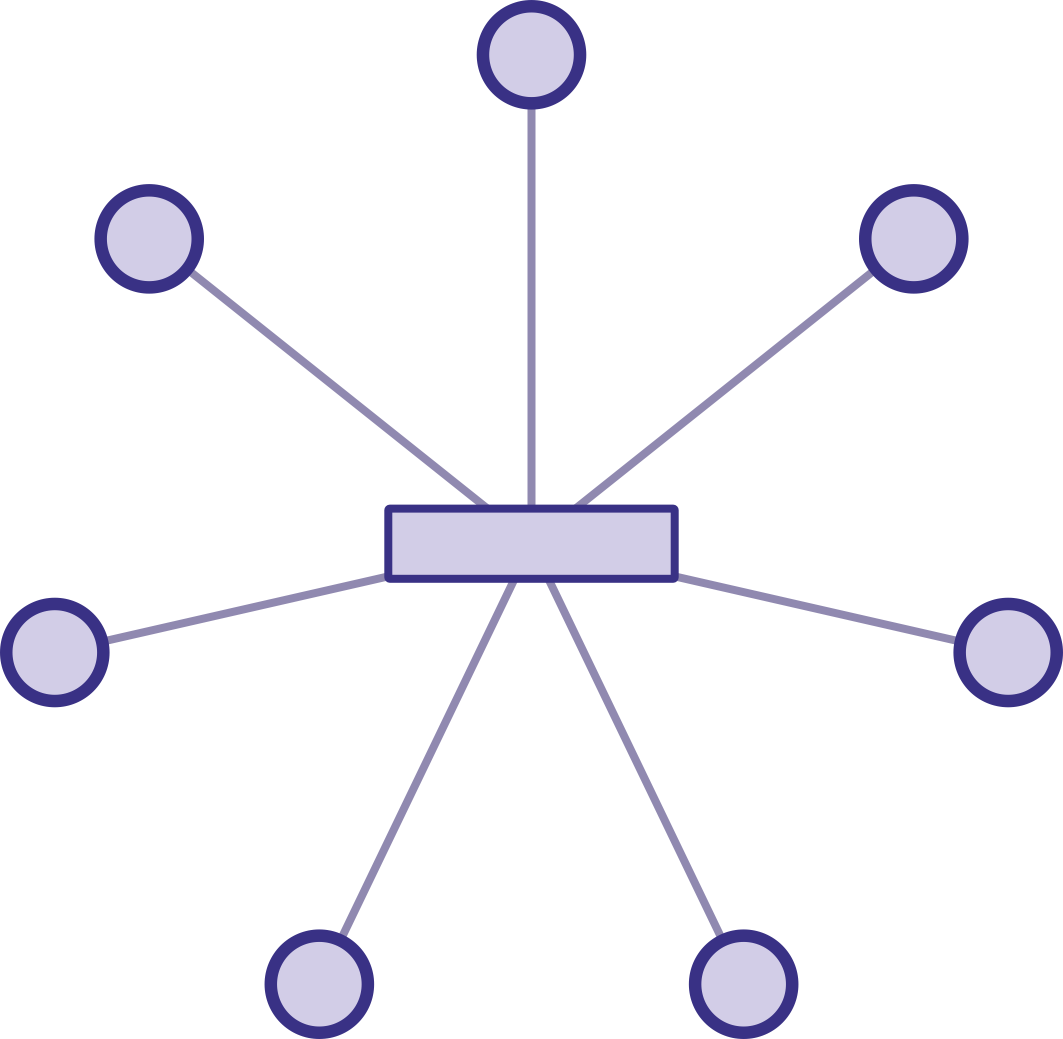
\includegraphics[width=0.4\textwidth]{imagenes/estrella.png}
    \caption{Topología en estrella}
    \label{fig:top_estrella}
\end{figure}

La topolog\'ia en estrella es la que menor gasto de energ\'ia desarrolla, pero por el contrario esta limitada por la
distancia de transmisi\'on v\'ia radio entre cada nodo y la puerta de enlace. Tampoco tiene un camino de comunicaci\'on alternativo en caso de que uno de los nodos tenga obstruido el camino de comunicaci\'on, lo que lleva a que en este caso la informaci\'on de ese nodo sea perdida.


\subsection{Topolog\'ia en malla}
La topolog\'ia en malla es un sistema multisalto, donde todos los nodos son routers y son id\'enticos. Cada nodo puede enviar y recibir informaci\'on de otro nodo y de la puerta de enlace. A diferencia de la topolog\'ia en estrella, donde los nodos solo pueden hablar con la puerta de enlace, en \'esta los nodos pueden enviarse mensajes entre ellos. 

\begin{figure}[htb]
    \centering
    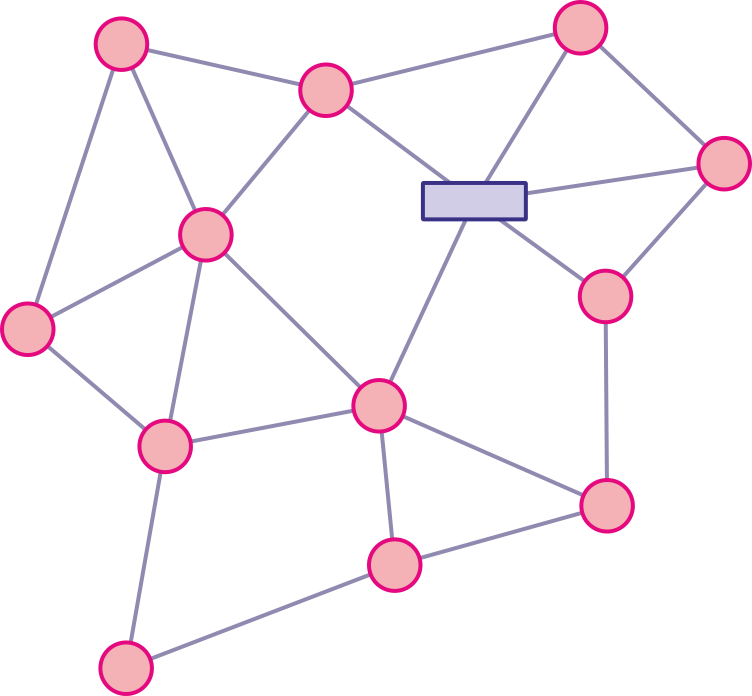
\includegraphics[width=0.6\textwidth]{imagenes/malla.png}
    \caption{Topología en malla}
    \label{fig:top_malla}
\end{figure}

La propagaci\'on de los datos a trav\'es de los nodos hacia la puerta de enlace hace posible, por lo menos en teor\'ia, crear una red con una extensi\'on posible ilimitada. Este tipo, tambi\'en es altamente tolerante a fallos ya que cada nodo tiene diferentes caminos para comunicarse con la puerta de enlace. Si un nodo falla, la red se reconfigurar\'a alrededor del nodo fallido autom\'aticamente. Dependiendo del n\'umero de nodos y de la distancia entre ellos, la red puede experimentar periodos de espera elevados a la hora de mandar la informaci\'on. 

\subsection{Topolog\'ia h\'ibrida (estrella-malla)}
Este tipo de red busca combinar las ventajas de los otros dos tipos, la simplicidad y el bajo consumo de una topolog\'ia en estrella, as\'i como la posibilidad de cubrir una gran extensi\'on y de reorganizarse ante fallos de la topolog\'ia en malla.

\begin{figure}[htb]
    \centering
    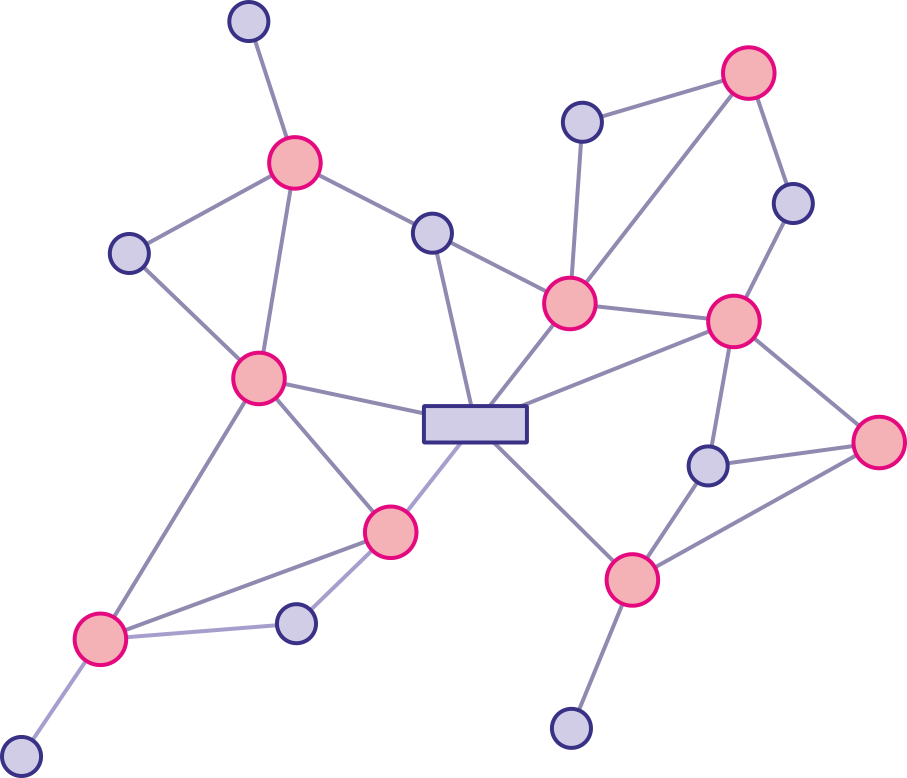
\includegraphics[width=0.7\textwidth]{imagenes/hibridamalla.png}
    \caption{Topología híbrida}
    \label{fig:top_hibrida}
\end{figure}

 Este tipo crea una red en estrella alrededor de routers pertenecientes a una red en malla. Los routers dan la
posibilidad de ampliar la red y de corregir fallos en estos nodos y los nodos finales se conectan con los routers
cercanos ahorrando energ\'ia.

\section {Redes ad-hoc y tecnolog\'ia inal\'ambrica} 

Las redes mas usadas en las implantaciones de redes de sensores inal\'ambricas son las redes malladas tipo ad-hoc. Son redes sin infraestructura, flexibles en las cuales todas las estaciones ofrecen servicios de encaminamiento para permitir la comunicaci\'on de estaciones que no tienen conexi\'on inal\'ambrica directa.

La principal caracter\'istica de las redes m\'oviles ad-hoc es que todos los dispositivos que forman parte de la red, adem\'as de funcionar como terminales finales, realizan tambi\'en funciones de retransmisi\'on de paquetes t\'ipicamente asociadas a routers. Esta cualidad nos permite encaminar paquetes a destinos sin cobertura directa a trav\'es de otros nodos intermedios que se encuentren en la red. De este modo se nos ofrece la posibilidad de incrementar de una manera extraordinaria la movilidad y el tama\~no de una red de datos inal\'ambrica. 

La funcionalidad principal de estas redes es la de crear de una manera r\'apida y eficaz una red temporal en lugares carentes de una infraestructura de red. Las principales caracter\'isticas de una red ad-hoc son: 

\begin{description}

\item[Movilidad]
Este aspecto es la raz\'on de ser de las redes ad-hoc. Los nodos se pueden reposicionar o simplemente ser m\'oviles, siempre que no salgan del alcance radio. Se pueden desplegar r\'apidamente sin la necesidad de descubrir la zona o formar grupos, es decir, cada nodo es individual y solvente. 

\item[Multisalto (Multihopping)]
Una red multihopping es una red donde el camino de la fuente al destino atraviesa varios nodos intermedios. 

\item[Autoorganizaci\'on]
La red de forma aut\'onoma debe determinar sus propios par\'ametros de configuraci\'on: direcci\'on, encaminamiento, clustering, indicador de posici\'on, etc. 

\item[Conservaci\'on de la energ\'ia] 
Los nodos m\'oviles, tienen una bater\'ia limitada y a no ser que dispongan de alg\'un mecanismo de carga (por ejemplo, un panel solar), no tienen capacidad de recarga. Es muy importante dise\~nar unos protocolos (MAC, encaminamiento) eficientes, con la finalidad de mejorar el rendimiento y prolongar la autonom\'ia de las bater\'ias. 

\item[Escalabilidad]
En algunos tipos de redes, el n\'umero de nodos puede crecer hasta llegar a varios miles. Como no existe un access point concreto, la incorporaci\'on y descarte de nodos es un proceso sencillo y transparente. 

\item[Seguridad]
Las redes inal\'ambricas son vulnerables a ataques, y las redes ad-hoc lo son especialmente. Pueden padecer tanto ataques activos como pasivos y el atacante puede emular a un nodo leg\'itimo y capturar paquetes de datos y control, destruir tablas de encaminamiento, etc.
\end{description}

\subsection{Protocolos}
Sin embargo, para que lo anterior sea viable se hace necesaria la inclusi\'on en la red de protocolos de encaminamiento que nos permitan crear las rutas hacia los destinos deseados. 

Los protocolos tradicionales propios de redes fijas no se adaptan bien a este tipo de entornos tan din\'amicos y, por tanto, ser\'a necesario el dise\~no espec\'ifico de protocolos para proporcionar un comportamiento eficiente a la red. 

La principal clasificaci\'on es la que diferencia entre protocolos proactivos y reactivos (o bajo demanda): 

Los protocolos proactivos, peri\'odicamente se env\'ia informaci\'on de encaminamiento para que en cualquier momento cualquier nodo pueda comunicarse con cualquier otro de la red. Esta caracter\'istica proporciona una r\'apida respuesta ante solicitudes de ruta y ofrece un buen comportamiento en situaciones donde la tasa de movilidad es alta. Sin embargo la sobrecarga que se introduce en la red con informaci\'on de control es alta. Entre estos protocolos podemos destacar el protocolo DSDV (Destination-Sequenced Distance Vector).

Por otra parte, los protocolos reactivos s\'olo crean rutas cuando es necesario. Son protocolos bajo demanda donde la sobrecarga es mucho menor, pero los retrasos de establecimiento de rutas son mayores. Podemos nombrar AODV (Ad hoc On-Demand Distance Vector) como protocolo reactivo. Existen algunos protocolos h\'ibridos en los que se mantiene una filosof\'ia proactiva en un \'ambito local y reactiva a nivel m\'as global, como el protocolo ZRP (Zone Routing Protocol).

Los principales protocolos utilizados son:

\begin{description}
\item[Destination-Sequenced Distance Vector (DSDV)] 
DSDV es esencialmente una modificaci\'on del algoritmo de encaminamiento Vector Distancia Bell-man-Ford, bien conocido por su utilidad en redes fijas, como por ejemplo en el protocolo RIP. 

En este algoritmo, los nodos vecinos intercambian peri\'odicamente (proactivo) sus tablas de encaminamiento enteras para estimar la distancia a la que se encuentran los dem\'as nodos no vecinos. Las modificaciones introducidas por DSDV proporcionan b\'asicamente la obtenci\'on de rutas sin bucles mediante la introducci\'on de n\'umeros de secuencia para la determinaci\'on de las rutas m\'as nuevas. Aunque DSDV s\'olo proporciona un camino para cada destino, siempre elige el camino m\'as corto bas\'andose en el n\'umero de saltos hacia este destino.

 DSDV utiliza dos tipos de mensajes de actualizaci\'on, uno m\'as grande (full-dump) y otro mucho m\'as peque\~no (incremental). Los mensajes incrementales pueden utilizarse para actualizaciones intermedias entre env\'ios peri\'odicos (full-dump) de la tabla entera de encaminamiento. Adem\'as se realizan estimaciones de los tiempos de establecimientos de ruta que retrasar\'an el env\'io de mensajes incrementales para evitar env\'ios en cadena de estos mensajes. 

\item[Optimized Link-State Routing Algorithm (OLSR)]
OLSR incorpora la filosof\'ia utilizada en protocolos tradicionales como OSPF de Estado de los Enlaces. En este algoritmo todos los nodos se intercambian mensajes para formarse una visi\'on consistente de toda la red y as\'i poder decidir el encaminamiento de paquetes.

 OLSR adolece del mismo problema que DSDV debido a la necesidad de intercambio de un gran n\'umero de mensajes peri\'odicos (proactivo). Aqu\'i, el problema podr\'ia llegar a ser mayor, ya que adem\'as de mensajes [91?]hello[92?] a los vecinos, env\'ia mensajes de control [91?]tc[92?] (Topology Control) que se retransmiten a todos los nodos de la red. 
 
 Sin embargo se ha conseguido una gran optimizaci\'on en la retransmisi\'on de estos mensajes con la incorporaci\'on de la t\'ecnica de retransmisi\'on multipunto, a trav\'es de la cual, los mensajes s\'olo son retransmitidos por el m\'inimo n\'umero de nodos necesarios para alcanzar a todos los dem\'as. Estos nodos son conocidos como grupo de retransmisores multipunto (MPR's). 

\item[Dynamic Source Routing (DSR)]
El protocolo DSR se fundamenta en el encaminamiento desde el origen, es decir, los paquetes de datos incluyen una cabecera de informaci\'on acerca de los nodos exactos que deben atravesar. No requiere ning\'un tipo de mensajes peri\'odicos (reactivo), disminuyendo as\'i la sobrecarga con mensajes de control. Adem\'as ofrece la posibilidad de obtener, con la solicitud de una ruta, m\'ultiples caminos posibles hacia el destino.

 Tampoco son un problema, a diferencia de la mayor\'ia de protocolos de encaminamiento en este tipo de redes, los enlaces unidireccionales. Para poder realizar el encaminamiento en el origen, a cada paquete de datos se le inserta una cabecera DSR de opciones que se colocar\'a entre la cabecera de transporte y la IP. Entre dichas opciones se incluir\'a la ruta que debe seguir el paquete nodo a nodo. 
 
 Cada nodo mantiene una memoria cach\'e de rutas en la que se van almacenando las rutas obtenidas a trav\'es de procesos de descubrimiento de rutas ya sean propias o obtenidas a trav\'es de escuchas en la red. En los procesos de descubrimiento de rutas se generan mensajes de solicitud, respuesta y error siendo estos mensajes route request, reply y error respectivamente. 

\item[Ad Hoc On-Demand Distance Vector (AODV)]
En el protocolo AODV los nodos mantienen una tabla de encaminamiento para los destinos conocidos (empleando el algoritmo vector distancia). Inicialmente esta tabla estar\'a formada por sus vecinos. Solamente se le a\~nadir\'an destinos nuevos cuando sea necesario, es decir, cuando un nodo necesita comunicarse con otro que no est\'a en su tabla, inicia un proceso de descubrimiento de ruta (reactivo) hacia el destino concreto.

Para ello se emiten mensajes de descubrimiento de ruta rreq que se van propagando entre todos los nodos de modo similar al DSR. En cambio, aqu\'i los nodos generan una tabla de encaminamiento inversa para que puedan regresar las contestaciones rrep a las solicitudes de ruta al nodo que la origin\'o. Se recomienda el uso de mensajes hello entre vecinos para determinar la conectividad, aunque para reducir el volumen de estos mensajes, s\'olo debe permitirse su env\'io a los nodos que est\'en transmitiendo datos. 

Debemos destacar adem\'as la utilizaci\'on de las t\'ecnicas de <<b\'usqueda secuencial por anillos>> y <<reparaci\'on local del enlace>> as\'i como tambi\'en que es capaz de proporcionar soporte multicast.
\end{description}

\subsection{Tecnolog\'ia inal\'ambrica}
Las tecnolog\'ias inal\'ambricas pueden clasificarse en cinco grandes grupos, de acuerdo con la distancia que viaja cada tipo de se\~nal.

Primero est\'an las comunicaciones satelitales, como el sistema de posicionamiento global (GPS, por sus siglas en ingl\'es), formado por 24 sat\'elites, los cuales env\'ian constantemente se\~nales a dispositivos en tierra. Sin embargo, estas se\~nales s\'olo viajan del sat\'elite al aparato receptor.

Otra categor\'ia, y con se\~nales de dos v\'ias, est\'an las tecnolog\'ias de telefon\'ia movil de cobertura amplia como GSM y CDMA. Entre las versiones avanzadas de tercera generaci\'on (3G) destacan HSDPA y LTE.

Una tercera categor\'ia incluye se\~nales de menor alcance utilizadas para conectar dispositivos dentro de una habitaci\'on o un edificio, como los sistemas Wi-Fi para conectarse a Internet dentro de hoteles o aeropuertos, o Zigbee, protocolo de comunicaciones inal\'ambricas que sirve para interconectar sensores.

En cuarto lugar est\'an los protocolos para enlazar dispositivos en una <<red de \'area personal>> (PAN, personal area network). Por ejemplo Bluetooth, utilizado para enviar la se\~nal de un tel\'efono movil a un auricular inal\'ambrico. 

El \'ultimo tipo de comunicaciones son las que se dan cerca de una antena transmisora (NFC, near-field communications). En este caso, el dispositivo receptor debe estar cerca del sistema emisor, por ejemplo, al pasar por un edificio o en el transporte p\'ublico.

Estos sistemas de radio son tan diferentes entre s\'i como la luz lo es del sonido. En la figura \ref{fig:tecinalamb} Podemos ver como se distribuyen las diferentes tecnolog\'ias inal\'ambricas dependiendo de la velocidad de transmisi\'on y de su utilizaci\'on.


 

\begin{figure}[ht]
    \centering
    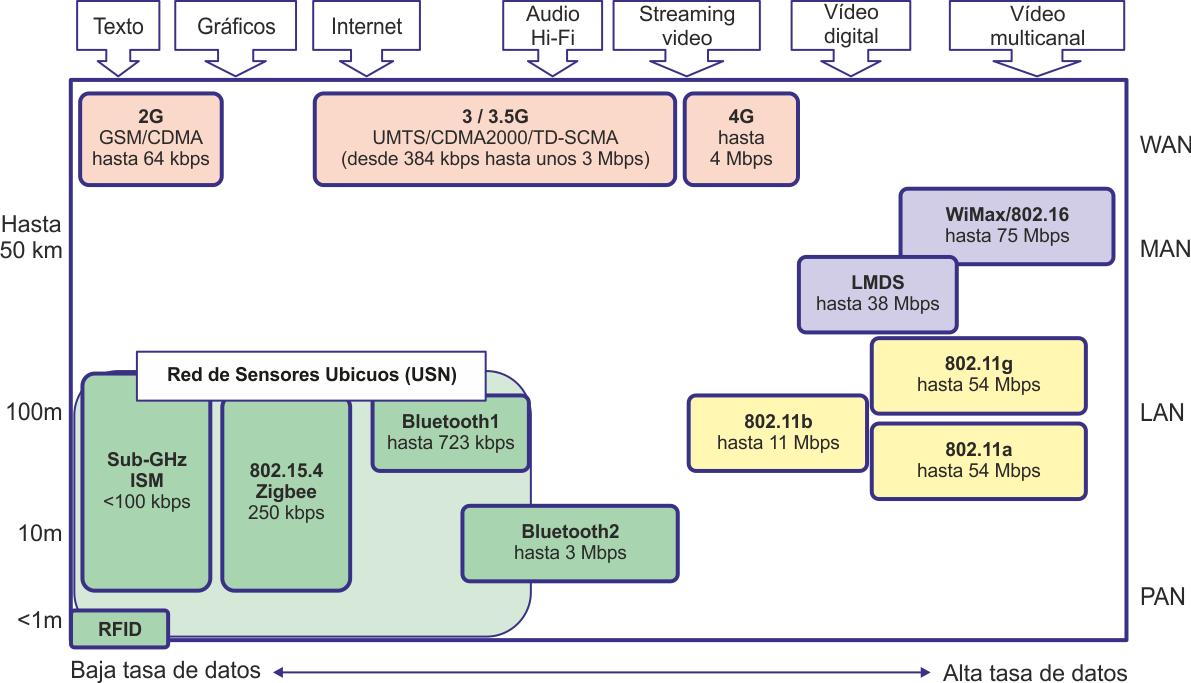
\includegraphics[width=0.8\textwidth]{imagenes/tec-inalamb.png}
    \caption{Distribución tecnologías inalámbricas}
    \label{fig:tecinalamb}
\end{figure}


 

Claramente se ve que los protocolos m\'as adecuados para ser usados en WSN son los protocolos Bluetooth y Zigbee. A pesar de que ZigBee es muy similar a Bluetooth podemos encontrar algunas diferencias que hacen m\'as adecuado el protocolo Zigbee para las WSN: 

\begin{itemize}
\item Una red ZigBee puede constar de un m\'aximo de 65535 nodos distribuidos en subredes de 255 nodos, frente a los 8 m\'aximos de una subred Bluetooth. 
\item Zigbee tiene un menor consumo el\'ectrico que el Bluetooth. Este menor consumo se debe a que el sistema ZigBee se queda la mayor parte del tiempo dormido, mientras que en una comunicaci\'on Bluetooth esto no se puede dar, y siempre se est\'a transmitiendo y/o recibiendo.
\end{itemize}



\subsection{Zigbee}
ZigBee es el nombre de la especificaci\'on de un conjunto de protocolos de alto nivel de comunicaci\'on inal\'ambrica para su utilizaci\'on con radiodifusi\'on digital de bajo consumo, basada en el est\'andar IEEE 802.15.4 de redes inal\'ambricas de \'area personal (wireless personal area network, WPAN).

Su objetivo son las aplicaciones que requieren comunicaciones seguras con baja tasa de env\'io de datos y maximizaci\'on de la vida \'util de sus bater\'ias.

En principio, el \'ambito donde se prev\'e que esta tecnolog\'ia cobre m\'as fuerza es en dom\'otica, como puede verse en los documentos de la ZigBee Alliance, la raz\'on de ello son diversas caracter\'isticas que lo diferencian de otras tecnolog\'ias:

\begin{itemize}
\item Su bajo consumo.
\item Su topolog\'ia de red en malla.
\item Su f\'acil integraci\'on (se pueden fabricar nodos con muy poca electr\'onica).
\end{itemize}
ZigBee utiliza la banda ISM para usos industriales, cient\'ificos y m\'edicos; en concreto, 868 MHz en Europa, 915 en Estados Unidos y 2,4 GHz en todo el mundo. Sin embargo, a la hora de dise\~nar dispositivos, las empresas optar\'an pr\'acticamente siempre por la banda de 2,4 GHz, por ser libre en todo el mundo.

El desarrollo de la tecnolog\'ia se centra en la sencillez y el bajo costo m\'as que otras redes inal\'ambricas semejantes de la familia WPAN, como por ejemplo Wi-Fi o Bluetooth. El nodo ZigBee m\'as completo requiere en teor\'ia cerca del 10\% del hardware de un nodo Bluetooth o Wi-Fi t\'ipico.

\subsubsection{Tipos de dispositivos}
Se definen tres tipos distintos de dispositivo ZigBee seg\'un su papel en la red:

\begin{itemize}
\item Coordinador ZigBee (ZigBee Coordinator, ZC): el tipo de dispositivo m\'as completo. Debe existir al menos uno por red. Sus funciones son las de encargarse de controlar la red y los caminos que deben seguir los dispositivos para conectarse entre ellos.
\item Router ZigBee (ZigBee Router, ZR): interconecta dispositivos separados en la topolog\'ia de la red, adem\'as de ofrecer un nivel de aplicaci\'on para la ejecuci\'on de c\'odigo de usuario.
\item Dispositivo final (ZigBee End Device, ZED): posee la funcionalidad necesaria para comunicarse con su nodo padre (el coordinador o un router), pero no puede transmitir informaci\'on destinada a otros dispositivos. De esta forma, este tipo de nodo puede estar dormido la mayor parte del tiempo, aumentando la vida media de sus bater\'ias. Un ZED tiene requerimientos m\'inimos de memoria y es por tanto significativamente m\'as barato.
\end{itemize}
Como ejemplo de aplicaci\'on en Dom\'otica, en una habitaci\'on de la casa tendr\'iamos diversos Dispositivos Finales (como un interruptor y una l\'ampara) y una red de interconexi\'on realizada con Routers ZigBee y gobernada por el Coordinador.

Bas\'andose en su funcionalidad, puede plantearse una segunda clasificaci\'on:

\begin{itemize}
\item Dispositivo de funcionalidad completa (FFD): Tambi\'en conocidos como nodo activo. Es capaz de recibir mensajes en formato 802.15.4. Gracias a la memoria adicional y a la capacidad de computar, puede funcionar como Coordinador o Router ZigBee, o puede ser usado en dispositivos de red que act\'uen de interfaz con los usuarios.
\item Dispositivo de funcionalidad reducida (RFD): Tambi\'en conocido como nodo pasivo. Tiene capacidad y funcionalidad limitadas (especificada en el est\'andar) con el objetivo de conseguir un bajo coste y una gran simplicidad. B\'asicamente, son los sensores/actuadores de la red.
\end{itemize}



\subsubsection{Estrategias de conexi\'on de los dispositivos}
Las redes ZigBee han sido dise\~nadas para conservar la potencia en los nodos <<esclavos>>. De esta forma se consigue el bajo consumo de potencia. La estrategia consiste en que, durante mucho tiempo, un dispositivo
<<esclavo>> est\'a en modo <<dormido>>, de tal forma que solo se <<despierta>> por una fracci\'on de segundo para confirmar que est\'a <<vivo>> en la red de dispositivos de la que forma parte. Esta transici\'on del modo <<dormido>> al modo <<despierto>> (modo en el que realmente transmite), dura unos 15ms, y la enumeraci\'on de <<esclavos>> dura alrededor de 30ms, como ya se ha comentado anteriormente.1

En las redes Zigbee, se pueden usar dos tipos de entornos o sistemas:

\begin{description}
\item[Con balizas] Es un mecanismo de control del consumo de potencia en la red. Permite a todos los dispositivos saber cu\'ando pueden transmitir. En este modelo, los dos caminos de la red tienen un distribuidor que se encarga de controlar el canal y dirigir las transmisiones.

 Las balizas que dan nombre a este tipo de entorno, se usan para poder sincronizar todos los dispositivos que conforman la red, identificando la red dom\'otica, y describiendo la estructura de la <<supertrama>>. Los intervalos de las balizas son asignados por el coordinador de red y pueden variar desde los 15ms hasta los 4 minutos.Este modo es m\'as recomendable cuando el coordinador de red trabaja con una bater\'ia.
 
  Los dispositivos que conforman la red, escuchan a dicho coordinador durante el <<balizamiento>> (env\'io de mensajes a todos los dispositivos -broadcast-, entre 0,015 y 252 segundos). Un dispositivo que quiera intervenir, lo primero que tendr\'a que hacer es registrarse para el coordinador, y es entonces cuando mira si hay mensajes para \'el. En el caso de que no haya mensajes, este dispositivo vuelve a <<dormir>>, y se despierta de acuerdo a un horario que ha establecido previamente el coordinador. En cuanto el coordinador termina el <<balizamiento>>, vuelve a <<dormirse>>.
  
\item[Sin balizas] Ee usa el acceso m\'ultiple al sistema Zigbee en una red punto a punto cercano. En este tipo, cada dispositivo es aut\'onomo, pudiendo iniciar una conversaci\'on, en la cual los otros pueden interferir. A veces, puede ocurrir que el dispositivo destino puede no o\'ir la petici\'on, o que el canal est\'e ocupado.Este sistema se usa t\'ipicamente en los sistemas de seguridad, en los cuales sus dispositivos (sensores, detectores de movimiento o de rotura de cristales), duermen pr\'acticamente todo el tiempo (el 99,999\%). Para que se les tenga en cuenta, estos elementos se <<despiertan>> de forma regular para anunciar que siguen en la red. 

Cuando se produce un evento (en nuestro sistema ser\'a cuando se detecta algo), el sensor <<despierta>> instant\'aneamente y transmite la alarma correspondiente. Es en ese momento cuando el coordinador de red, recibe el mensaje enviado por el sensor, y activa la alarma correspondiente. En este caso, el coordinador de red se alimenta de la red principal durante todo el tiempo.
\end{description}

\subsubsection{Comunicaci\'on y descubrimiento de dispositivos}
Seg\'un la informaci\'on disponible, el descubrimiento de dispositivos puede adecuarse utilizando varios m\'etodos distintos.

Si se conoce la direcci\'on de red, se pide la direcci\'on IEEE utilizando unicast. Sino es as\'i, se pide por broadcast, y la direcci\'on IEEE forma parte de la respuesta. Los dispositivos hoja (end devices) responden con la direcci\'on propia solicitada, mientras que routers y coordinadores env\'ian tambi\'en las direcciones de todos los dispositivos asociados a ellos.

Este protocolo extendido permite indagar acerca de dispositivos dentro de una red y sus servicios ofrecidos a nodos externos a la misma. Los endpoints pueden informar acerca de estos servicios cuando el protocolo de descubrimiento dirige mensajes a ellos. Tambi\'en pueden utilizarse servicios de emparejamiento oferta-demanda.

Los identificadores de cluster favorecen la asociaci\'on entre entidades complementarias por medio de tablas de asociaci\'on, mantenidas en los coordinadores ZigBee ya que estas tablas siempre han de estar disponibles en una red (los coordinadores son, de entre todos los nodos, los que con mayor seguridad dispondr\'an de una alimentaci\'on continua). Los backups a estas tablas, de ser necesarios para la aplicaci\'on, han de realizarse en niveles superiores.

Por otra parte, el establecimiento de asociaciones necesita que se haya formado un enlace de comunicaci\'on; tras ello, se decide si adjuntar un nuevo nodo a la red en funci\'on de la aplicaci\'on y las pol\'iticas de seguridad.

Nada m\'as establecerse la asociaci\'on pueden iniciarse las comunicaciones. El direccionamiento directo utiliza la direcci\'on de radio y el n\'umero de endpoint; el indirecto necesita toda la informaci\'on relevante (direcci\'on, endpoint, cluster y atributo) y  la env\'ia al coordinador de la red, que mantiene esta informaci\'on por \'el y traduce sus peticiones de comunicaci\'on. Este direccionamiento indirecto es especialmente \'util para favorecer el uso de dispositivos muy sencillos y minimizar el almacenamiento interno necesario. 

Adem\'as de estos dos m\'etodos, se puede hacer broadcast a todos los endpoints de un dispositivo, y direccionamiento de grupos para comunicarse con grupos de endpoints de uno o varios dispositivos distintos.


\subsubsection{Protocolos}
Los protocolos se basan en algoritmos de red para la construcci\'on de redes ad-hoc de baja velocidad. La mayor\'ia de redes grandes est\'an pensadas para formar un cluster de clusters. Tambi\'en puede estructurarse en forma de malla o como un solo cluster. Los perfiles actuales de los protocolos soportan redes que utilicen o no facilidades de balizado.

Las redes sin balizas acceden al canal por medio de CSMA/CA. Los routers suelen estar activos todo el tiempo, por lo que requieren una alimentaci\'on estable en general. Esto, a cambio, permite redes heterog\'eneas en las que algunos dispositivos pueden estar transmitiendo todo el tiempo, mientras que otros s\'olo transmiten ante la presencia de est\'imulos externos. El ejemplo t\'ipico es un interruptor inal\'ambrico: un nodo en la l\'ampara puede estar recibiendo continuamente ya que est\'a conectado a la red; por el contrario, un interruptor a pilas estar\'ia dormido hasta que el mecanismo se activa. En una red as\'i la l\'ampara ser\'ia un router o coordinador, y el interruptor un dispositivo final.

Si la red utiliza balizas, los routers las generan peri\'odicamente para confirmar su presencia a otros nodos. Los nodos pueden desactivarse entre las recepciones de balizas reduciendo su ciclo de servicio (duty cycle). Sin embargo, los periodos largos con ciclos de servicio cortos necesitan que una temporizaci\'on precisa, lo que puede ir en contra del principio de bajo coste.

En general, los protocolos ZigBee minimizan el tiempo de actividad de la radio para evitar el uso de energ\'ia. En las redes con balizas los nodos s\'olo necesitan estar despiertos mientras se transmiten las balizas (adem\'as de cuando se les asigna tiempo para transmitir). Si no hay balizas, el consumo es asim\'etrico repartido en dispositivos permanentemente activos y otros que s\'olo no est\'an espor\'adicamente.

Las radios utilizan un espectro de dispersi\'on de secuencia directa. Se utiliza BPSK en los dos rangos menores de frecuencia, as\'i como un QPSK ortogonal que transmite dos bits por s\'imbolo en la banda de 2,4 GHz. Los rangos de transmisi\'on oscilan entre los 10 y 75 metros, aunque depende bastante del entorno. La potencia de salida de las radios suele ser de 0 dBm (1 mW).


	\chapter{Hardware}
Como hemos visto en el capitulo anterior el hardware que compone una red de sensores básicamente es de dos tipos: los nodos y el gateway. Buscaremos en el mercado los dispositivos que mejor se adecuen a nuestras necesidades. Empecemos con el hardware de los nodos.


\section{Nodos sensores}
Como primera opción veamos los principales nodos ya existentes en el mercado y los sistemas operativos que los gobiernan.



\subsection{Nodos en el mercado}
En estos nodos el popular uso del MSP430 y el ATmega128 como unidad microcontroladora se debe a varios factores, entre ellos: ultra bajo consumo de energía, soporte de la comunidad de desarrolladores, compiladores open-source basados en GNU GCC, y soporte de Tiny OS.



Existen también otros tipos de nodos basados en arquitecturas ARM como SunSpot de Sun Microsystems, e IMote2 de Crossbow. Estos proporcionan arquitecturas de 32 bits, velocidades de procesado mayores de 100MHz, unidades de manejo de memoria y la capacidad de soportar versiones ligeras de Linux.



El SunSpot de Sun Microsystem usa Squawk, una maquina virtual de Java que soporta Java nativo en un ATMEL920T ARM. Squawk es una MV de código abierto escrita mayormente en Java y que se ejecuta directamente sobre el microcontrolador sin la necesidad de un sistema operativo. Ejecutándose sin un SO subyacente se reducen los requisitos de memoria, la complejidad de la implementación, y la necesidad de soportar múltiples sistemas operativos. El hardware de este nodo es normalmente considerado de lujo en comparación con otros, con lo que el precio de estos puede subir fácilmente. La única característica que lo diferencia es que los nodos son programados en Java.



Las plataformas IRIS, MicaZ, Mica2, TelosB, IMote2 pertenecen a Crossbow. La tecnología desarrollada por esta empresa tiene su origen en las investigaciones de su fundador en la Universidad de California Berkeley, y ha estado a la vanguardia durante más de una década.



IRIS, MicaZ y Mica2 tienen unas especificaciones casi idénticas, ya que unas son revisiones de las otras. \ IRIS utiliza una versión ligeramente mejorada del ATmega128 de la MicaZ y tiene el doble SRAM interna. Mica2 usa el mismo microcontrolador de la MicaZ, pero con un radio transceptor de menor frecuencia. Además de algunas mejoras de hardware como más temporizadores, entrada/salida digitales, puertos SPI, etc... Todas soportan TinyOS y usan una red Zigbee.



La TelosB usa un microcontrolador de 16bit, el MSP430 de Texas Instruments, el cual pertenece a una de las familias de controladores más populares en la comunidad de investigación actual. TelosB también cuenta con conectividad directa a USB, para una programación y depuración fácil, así como cuatro sensores ya conectados que proveen que permiten al usuario leer y transmitir valores sin la necesidad de acoplarle sensores personalizados.



IMote2 esta esta basada en el procesador Intel Xcale PXA271 de arquitectura ARM. Esta no es una plataforma tradicional de bajo coste, consumo y recursos. De hecho, se centra en aplicaciones que requieren recursos computacionales altos, como procesado de video y audio. IMote2 soporta velocidades desde 13MHz hasta 416MHz y es una de las pocas que han portado TinyOS a un microcontrolador no MSP430 o Atmega. También soporta Linux y Microsoft .NET Microframework.




Por ultimo tenemos WaspMote de Libelium una empresa española. WaspMote es una evolución de la SquidBee basada en el tándem Arduino-Xbee, es completamente compatible con el código Arduino, salvando las diferencias del pinout, y soluciona el problema de poner el nodo en modo sleep, solo con Arduino no es posible. Además tiene una gran variedad de placas sensoras listas para acoplar y usar, y múltiples opciones de conectividad, como pueden ser: 802.15.4, ZigBee, Bluetooth, radiofrecuencia, etc...



En cuanto a precios estos oscilan entre los aproximadamente 150\euro del WaspMote a los 700\euro aproximadamente del SunSpot, eso solo las placas básicas, sin contar con los sensores que habría que instalarles.



\subsection{Sistemas Operativos para WSN}
Las necesidades que tiene un nodo de una WSN son totalmente distintas a las que pueda tener cualquier otro dispositivo como puede ser un PC, por lo tanto estos nodos tienen sus propios sistemas operativos.




Los sistemas operativos para WSN son típicamente menos complejos que los de propósito general, debido a los requisitos especiales de las aplicaciones en las que se usan, como a las restricciones de recursos encontradas en las plataformas hardware utilizadas. Por ejemplo, las aplicaciones de WSN no son interactivas como son las aplicaciones para PC y debido a esto, estos sistemas no necesitan incluir el soporte de interfaz de usuario. Además, las restricciones de los recursos en términos de memoria hacen imposible de implementar los mecanismos de memoria virtual.



El hardware de la redes inalámbricas de sensores no es muy diferente al de sistemas empotrados tradicionales y por lo tanto es posible utilizar sistemas como eCos o uC/OS. Sin embargo, estos sistemas están diseñados para usar operaciones en tiempo real. A diferencia de los tradicionales sistemas operativos para sistemas empotrados, los sistemas desarrollados para redes de sensores inalámbricas no tienen como objetivo apoyar operaciones en tiempo real.



TinyOS es quizás el primer sistema operativo diseñado específicamente para redes de sensores inalámbricas. A diferencia de la mayoría de los otros sistemas operativos, TinyOS se basa en un modelo de programación controlado por eventos en vez de multiprocesos. Los programas de TinyOS están compuestos por eventos y tareas guiadas. Cuando un evento externo ocurre, como puede ser la entrada de un paquete de datos o la lectura de un sensor, TinyOS llama al evento apropiado y lo ejecuta. El lanzador de eventos puede posponer tareas durante cierto tiempo. 



Tanto TinyOS como los programas escritos para él son escritos en un lenguaje de programación especial llamado nesC, que es una extensión del lenguaje de programación C. NesC esta diseñado para determinar las prioridades entre tareas y eventos.



Hay también sistemas operativos que permiten programar en C. Por ejemplo Contiki, MANTIS, Btnut, SOS y Nano-RK. Contiki esta diseñado para soportar la carga de módulos a través de la red y para soportar cargas de ficheros ELF. El kernel de Contiki esta basado en lanzamiento de eventos, como TinyOS, pero puede llegar a soportar multitareas básicas. 



A diferencia del kernel de Contiki basado en eventos, los kernels MANTIS y Nano-RK están basados en multitareas preventivas. El kernel divide el tiempo entre los procesos activos y decide que proceso debe ser ejecutado para hacer la programación de la aplicación más fácil. Nano-RK tiene un kernel basado en tiempo real que permite controlar la manera de acceder de las tareas, a la CPU, a la red y a las placas sensoras. 




Como TinyOS y Contiki, SOS es un sistema operativo basado en eventos. La principal característica de SOS es su soporte para módulos cargables. Un sistema complejo se construye a partir de módulos más pequeños, probablemente en tiempo de ejecución. Para soportar el dinamismo inherente en su modulo de interfaz, SOS soporta una gestión de la memoria dinámica.

 

\subsubsection{TinyOS}
TinyOS es un sistema operativo orientado a trabajar con redes de sensores, desarrollado en la Universidad de Berkeley. Puede ser visto como un conjunto de programas avanzados, el cual cuenta con un amplio uso por parte de comunidades de desarrollo, dada sus características de ser un proyecto de código abierto. Este ‘conjunto de programas’ contiene numerosos algoritmos, que nos permitirán generar enrutamientos, así como también aplicaciones pre-construidas para sensores. Además soporta diferentes plataformas de nodos de sensores, arquitecturas bases para el desarrollo de aplicaciones.



El lenguaje en el que se encuentra programado TinyOS es un meta-lenguaje que deriva de C, cuyo nombre es NesC. Además existen varias herramientas que ayudan el estudio y desarrollo de aplicaciones para las redes de sensores, que van desde aplicaciones para la obtención y manejo de datos, hasta sistemas completos de simulación.



El diseño de TinyOS está basado en responder a las características y necesidades de las redes de sensores, tales como reducido tamaño de memoria, bajo consumo de energía, operaciones de concurrencia intensiva, diversidad en diseños y usos, y finalmente operaciones robustas para facilitar el desarrollo confiable de aplicaciones. \ Además se encuentra optimizado en términos de uso de memoria y eficiencia de energía.



El diseño del Kernel de TinyOS está basado en una estructura de dos niveles de planificación:
\begin{description}
\item[Eventos] Pensados para realizar un proceso pequeño (por ejemplo cuando el contador del timer se interrumpe, o atender las interrupciones de un conversor análogo-digital). Además pueden interrumpir las tareas que se están ejecutando.
\item[Tareas] Las tareas son pensadas para hacer una cantidad mayor de procesamiento y no son críticas en tiempo (por ejemplo calcular el promedio en un arreglo). Las tareas se ejecutan en su totalidad, pero la solicitud de iniciar una tarea, y el término de ella son funciones separadas.
\end{description}



Con este diseño permitimos que los eventos (que son rápidamente ejecutables), puedan ser realizados inmediatamente, pudiendo interrumpir a las tareas (que tienen mayor complejidad en comparación a los eventos).



El enfoque basado en eventos es la solución ideal para alcanzar un alto rendimiento en aplicaciones de concurrencia intensiva. Adicionalmente, este enfoque usa las capacidades de la CPU de manera eficiente y de esta forma gasta el mínimo de energía.



TinyOS se encuentra programado en NesC, un lenguaje diseñado para reflejar las ideas propias del enfoque de componentes, incorporando además un modelo de programación que soporta concurrencia, manejo de comunicaciones y fácil interacción con el medio (manejo de hardware).



\subsubsection{LINUX}
Linux es un sistema operativo tipo Unix que se distribuye bajo la Licencia Pública General de GNU (GNU GPL), es decir que es software libre. Su nombre proviene del kernel de Linux, desarrollado en 1991 por Linus Torvalds.



Hablar de Linux es sólo referirse al Kernel, el núcleo del sistema. El núcleo sólo es una interfaz que permite comunicar el hardware con los programas. Por lo que el Kernel solo no forma el sistema operativo. 



Un sistema GNU/Linux empotrado simplemente hace referencia a un sistema empotrado basado en el kernel de Linux. Es importante destacar que no existe un kernel específico para sistemas empotrados, es decir, no necesitamos crear un kernel especial para sistemas empotrados. A menudo se utilizan las versiones oficiales del kernel de Linux para construir un sistema. Por supuesto, es necesario configurar el mismo para dar soporte especial al hardware de un determinado equipo.



 Fundamentalmente, un kernel utilizado en un sistema empotrado difiere de un kernel usado en una computadora de escritorio o servidor en la configuración del mismo al momento de compilarlo. 



La arquitectura de un sistema GNU/Linux está formado por un conjunto de componentes, y el kernel Linux es sólo una parte de este conjunto. Inmediatamente sobre el hardware se sitúa el kernel. El kernel es el componente central del sistema operativo. Sus funciones son principalmente administrar el hardware de manera coherente y justa mientras se le otorga un nivel de abstracción familiar, a través de las APIs, a las aplicaciones de nivel de usuario.




Entre otras tareas relevantes de un sistema operativo, el kernel Linux maneja dispositivos, administra los accesos de E/S, controla los procesos y administra el uso compartido de memoria. Dentro del kernel, la interfaz de bajo nivel es específica para cada configuración de hardware, sobre la cual, el kernel ejecuta y provee control directo de los recursos hardware. 



Típicamente, los servicios de bajo nivel manejan operaciones específicas de la CPU, operaciones de memoria específicas a la arquitectura, y provee interfaces básicas para dispositivos.



La capa de alto nivel provee abstracciones comunes a todos los sistemas Unix, incluyendo procesos, archivos, sockets y señales. Este nivel de abstracción se mantiene constante aunque difiera el hardware. 



Entre estos dos niveles de abstracción, el kernel necesita lo que se denomina componentes de interpretación para comprender e interactuar con datos estructurados provenientes de, o hacia ciertos dispositivos.



Los diferentes tipos de sistemas de archivos y los protocolos de red son ejemplos de fuentes de datos estructurados. El kernel necesita interpretarlos e interactuar a fin de proveer acceso a los datos provenientes desde estas fuentes o hacia las mismas.



\subsubsection{MICROSOFT .NET MICRO FRAMEWORK}
La .NET Micro Framework fue creada desde el inicio como una solución .NET para dispositivos integrados pequeños de sensores industriales e instrumentación para sistemas empotrados.



Además de estar totalmente integrada con Visual Studio, el kit de desarrollo de software .NET Micro Framework (SDK) viene equipado con un emulador extensible para simular capacidades de hardware. La estructura permite a los desarrolladores de dispositivos conectar diversas soluciones de hardware para prácticamente cualquier dispositivo periférico mediante conexiones de comunicación estándares de la industria y unidades gestionadas personalizadamente.




La .NET Micro Framework dispone de ofertas integradas de Microsoft en un nuevo mercado de dispositivos que se basan en procesadores de 32 bits de bajo coste y están constreñidos en términos de memoria, potencia de la batería y otros recursos. Ofreciendo paradigmas de programación potentes y modernos a este terreno, .NET Micro Framework pretende acelerar la innovación de dispositivos pequeños y conectados.

\begin{itemize}
\item Requiere sólo unos pocos cientos de kilobytes de RAM, y tan poco como 512 K de memoria flash.
\item Soporta procesadores con y sin MMU.
\item Dispone de una interfaz de control de energía que permite que la aplicación maximice la vida dela batería.
\end{itemize}


Hasta ahora la gente de Microsoft a publicado el SDK del Microsoft .NET Micro Framework 2.5 el cual nos permitirá desarrollar aplicaciones para pequeños dispositivos utilizando para tal motivo, Visual Studio, C\#. 



Microsoft .NET Micro Framework es un pequeño subconjunto reducido de clases, en donde podemos desarrollar soluciones en C\# para pequeños dispositivos, para trabajar con este pequeño Framework necesitamos disponer de Microsoft Visual Studio 2005 Standar o superior, y un sistema operativo Windows, los cuales suelen disponer de un conjunto de librerías .NET completamente integradas enfocadas al uso en sistemas empotrados.



Varias empresas están apostando por esta tecnología, Digi International Inc dio a conocer sus planes para un lanzamiento previo del kit de desarrollo Digi Connect ME para Microsoft .NET Micro Framework. El Digi Connect ME incluye soporte para redes Ethernet, un puerto en serie y señales de propósitos generales entrada/salida (GPIO). Es la primera solución disponible para .NET Micro Framework para dar apoyo a las redes Ethernet.



EmbeddedFusion, que entrega soluciones centrales de hardware y software integrado para desarrolladores de sistemas integrados, anunció el Meridian CPU, que es un módulo central CPU que incorpora procesador Freescale i.MXS, RAM, Flash y .NET Micro Framework. \ Para asistir a los desarrolladores en el aprendizaje de cómo se aplica .NET Micro Framework en varios escenarios integrados, EmbeddedFusion también creó la plataforma de desarrollo Tahoe, que permite la experimentación y exploración de .NET Micro Framework justo fuera de la caja.



Freescale también introdujo un kit de desarrollo para .NET Micro Framework que permite a los clientes entregar soluciones diferenciadas en el mercado con rendimiento ARM9 a muy baja potencia.



Además, Rhode Consulting, un especialista en tecnologías Microsoft Windows Embedded, anunció la disponibilidad del kit de evaluación de FlexiDis con .NET Micro Framework instalado. La plataforma FlexiDis utiliza los procesadores centrales Atmel ARM7 y ARM9 con velocidad de hasta 180 MHz. La combinación de esas velocidades, hasta 16 MB de memoria flash y SDRAM, y una pantalla QVGA de 2,2 hace de FlexiDis un componente de elección para varios tipos de aplicaciones industriales en las que se requieren HMI integrado o soluciones de visualización.




\subsubsection{eCos}
eCos (embedded Configurable operating system) es un sistema operativo de código abierto, gratuito y de operación en tiempo real desarrollado para sistemas empotrados y para aplicaciones que necesiten un procesador con múltiples sesiones. Puede ser personalizado para cumplir los requisitos que la aplicación precise, con cientos de opciones, pudiendo llegar a la mejor combinación entre el rendimiento en tiempo real y el hardware necesario.



Este sistema es programable bajo lenguaje C y tiene capas y APIs compatibles para POSIX y uITRON. eCos fue diseñado para aparatos con un tamaño de memoria sobre cientos de kilobytes o con requerimientos en tiempo real. Puede ser usado en hardware con muy poca RAM soportando Linux empotrado a partir de un mínimo de 2 MB de RAM, sin incluir las necesidades de la aplicación y del servicio.




eCos funciona correctamente en una amplia variedad de plataformas hardware como pueden ser, ARM, CalmRISC, FR-V, Hitachi H8, IA-32, Motorola 68000, Matsushita AM3x, MIPS, NEC V8xx, Nios II, PowerPC, SPARC, and SuperH.



Incluido con la distribución de eCos disponemos de RedBoot, una aplicación de código abierto que usa la capa de abstracción de hardware de eCos que provee soporte de arranque para sistemas empotrados.



eCos fue inicialmente desarrollado por Cygnus Solutions, que más tarde fue comprado por Red Hat. A principio de 2002 cesó el desarrollo de eCos y colocó al personal que estaba trabajando en el proyecto formando su propia compañía, eCosCentric, para continuar con su desarrollo y dar soporte comercial para eCos. En enero de 2004, a partir de una solicitud de los desarrolladores de eCos, Red Hat aceptó transferir los derechos de eCos a la Fundación de Software Libre. Esta transferencia fue finalmente ejecutada en octubre de 2005.



eCosPro está formado por una distribución de eCos y RedBoot creada por eCosCentric y está orientado a desarrolladores que quieran integrar eCos y RedBoot dentro de productos comerciales. Está definido como estable, completamente testado, certificado y con soporte, sin embargo, algunas de sus características no han sido liberadas como software libre.



\subsubsection{\(\mu\)C/OS}
MicroC/OS-II (comúnmente llamado \(\mu\)C/OS-II o uC/OS-II), es un sistema operativo multitarea, en tiempo real, basado en prioridad preventiva, de bajo coste donde el kernel está escrito principalmente en el lenguaje de programación C. Es principalmente entendido para uso en sistemas empotrados.



La designación II es debido a que es la segunda generación de un kernel que originalmente fue publicado en 1992 en la segunda parte de un articulo en la revista Embedded Systems Programming bajo el titulo \(\mu\)C/OS The Real-Time Kernel y escrito por Jean J. Labrosse. El autor intentó describir como funciona un sistema operativo portable por dentro y las razones por las que fue desarrollado. Pero rápidamente todo esto tomó un rumbo comercial.



\(\mu\)C/OS-II es soportado por Micrium Inc y se obtiene bajo licencia del producto, aunque el uso de este sistema operativo es gratis para uso educacional o no comercial. Adicionalmente Micrium distribuye otros productos de software como uC/OS-View, uC/CAN, uC/TCP-IP, uC/FS, uC/GUI, uC/MOD-BUS, uC/LCD, uC/USB (Mass Storage Device and Bulk) y un largo grupo de aplicaciones para uC/TCP-IP como software cliente para DHCP, POP3, SNTP, FTP, TFTP, DNS, SMTP, y TTCP. El software en su modalidad de servido incluye HTTP, FTP y TFTP. PPP es también disponible.



Está disponible para la mayor cantidad de procesadores y placas que existen en el mercado y es adecuado para el uso en sistemas empotrados donde la seguridad es crítica como en aviación, sistemas médicos o instalaciones nucleares.



\subsubsection{Contiki}
Contiki es un pequeño sistema operativo de código abierto, altamente portable y multitarea, desarrollado para uso en pequeños sistemas, desde ordenadores de 8-bit a sistemas empotrados sobre microcontroladores, incluyendo nodos de redes de sensores. El nombre Contiki viene de la famosa balsa Kon-Tiki de Thor Heyerdahl.




A pesar de incluir multitarea y una pila TCP/IP, Contiki sólo requiere varios kilobytes de código y unos cientos de bytes de RAM. Un sistema totalmente completo con una GUI requiere aproximadamente 30 kilobytes de RAM.

El núcleo básico y la mayor parte de las funciones principales fueron desarrolladas por Adam Dunkels en el grupo de sistemas de redes empotradas en el instituto sueco de ciencias computacionales.




Contiki consiste en un núcleo orientado a eventos, el cual hace uso de protohilos, sobre el cual los programas son cargados y descargados dinámicamente. También soporta multihilado apropiativo opcional por proceso, comunicación entre procesos mediante paso de mensajes a través de eventos, al igual que un subsistema GUI opcional, el cual puede usar un soporte directo de gráficos para terminales locales, terminales virtuales en red mediante VNC o sobre Telnet.



Contiki funciona en una variedad de plataformas, desde microcontroladores empotrados, como el MSP430 y el AVR, a viejas computadoras domésticas. El tamaño del código está en el orden de los kilobytes y el uso de la memoria puede configurarse para que sea de sólo unas decenas de bytes.

\subsubsection{MANTIS}
El sistema operativo MANTIS (MultimodAl system for NeTworks of In-situ wireless Sensors) suministra un nuevo sistema operativo empotrado de plataforma múltiple para redes de sensores inalámbricos. 



Ante el incremento de complejidad de las tareas realizadas por las redes de sensores como compresión, agregación y procesado de señales, los multiprocesos en MANTIS sensor OS (MOS) permiten interpaginar complejas tareas con tareas susceptibles al tiempo para así mitigar los problemas en los saltos de buffers.




Para conseguir una eficiencia en el uso de la memoria, MOS es implementado para que utilice una pequeña cantidad de RAM. Usando menos de 500 bytes de memoria, incluyendo el kernel, los controles de tiempo y la pila de comunicación. Para conseguir la eficiencia energética, el controlador de eficiencia energética de MOS hace que el microcontrolador duerma después de ejecutar todas las tareas activas, reduciendo el consumo de energía al rango de \(\mu\)A.



Una de las características principales de MOS es la flexibilidad en el soporte de múltiples plataformas como PCs, PDAs y diferentes plataformas de microsensores. Otra de las características destacada del diseño de MOS es el soporte de control remoto, permitiendo una reprogramación dinámica y un acceso remoto.



\subsubsection{BTnut}
Sistema operativo de código abierto creado para correr dentro de sistemas empotrados BTnodes. Fue diseñado principalmente para el procesador Atmel ATmega128 (el cual forma parte de los motes BTnodes) y por lo tanto es el más recomendado para esta clase de nodos.



La actual compilación de sus programas (la conversión de código C a código maquina) es realizada usado gcc-avr, el cual es un compilador de C libre para la plataforma de procesadores Atmel. Podemos diferenciar tres partes: las rudimentarias librerías C que son implementadas por la parte avr-libc de gcc-avr; las rutinas de alto nivel construidas para avr-libc por Nut/OS; y los drivers específicos para el funcionamiento del mote BT-node proporcionados por BTnut.



\subsubsection{SOS}
SOS es un sistema operativo desarrollado en la Universidad de California (UCLA), específicamente en el NESL (Networked \& Embedded Systems Laboratory).



SOS es un sistema operativo para redes de sensores que procura remediar algunos de las limitaciones propias de la naturaleza estática de muchos de los sistemas precursores a éste (por ejemplo TinyOS).



SOS implementa un sistema de mensajería que permite múltiples hebras entre la base del sistema operativo y las aplicaciones, las cuales pasan a ser módulos que pueden ser cargadas o descargadas en tiempo de ejecución sin interrumpir la base del sistema operativo.



El principal objetivo de SOS es la reconfigurabilidad. Ésta se define como la habilidad para modificar el software de nodos individuales de una red de sensores, una vez que estos han sido desplegados físicamente e inicializado su funcionamiento. En el caso de encontrar un problema, en caso de no contar con esta solución, habría sido necesario recolectar todos los nodos para poder modificar su software.



La capacidad de dinámicamente agregar o remover módulos, permite la construcción de software mucho más tolerante a fallos. Esto presenta dos grandes ventajas: una es el hecho de poder realizar updates fácilmente, y la otra es la capacidad de anular el funcionamiento de algún módulo defectuoso, de algún nodo que pertenece a la red.



Además de las técnicas tradicionales usadas en el diseño de sistemas empotrados, las características del kernel de SOS son:
\begin{itemize}
\item Módulos cargados dinámicamente.
\item Programación flexible de prioridades.
\item Simple subsistema de memoria dinámica.
\end{itemize}






\subsubsection{Nano-RK}
Nano-RK es un sistema operativo completamente preventivo basado en reserva bajo tiempo real (RTOS) desarrollado en la universidad de Carnegie Mellon con soporte para redes multisalto adecuado para el uso en redes de sensores inalámbricas. Nano-RK funciona adecuadamente con plataformas como redes de sensores FireFly y sobre los motes MicaZ.



Incluye un kernel con recursos empotrados de bajo peso con bastantes funcionalidades y soporte de tiempo usando menos de 2 KB de memoria RAM y 18 KB de ROM. Nano-RK soporta multitareas preventivas con prioridad para asegurar que los plazos de las tareas son conocidos, además de soporte de CPU, red y sensores y actuadores.



Las tareas pueden especificar las demandas de recursos y el sistema operativo provee el acceso controlado y garantizado para los ciclos de CPU y los paquetes de red. Todos estos recursos forman la reserva de energía virtual que permite al sistema operativo controlar el nivel de energía del sistema y de las tareas.



\subsection{Conclusión}
Después de haber analizado muchos de los nodos existentes y sus sistemas operativos, vemos que estos pueden llegar a ser bastante caros. además, al estar orientados a los ámbitos académicos e industriales, no son fácilmente operables por usuarios no versados en el tema de las WSN, aparte de que seria complicado acceder a este tipo de hardware por estos usuarios.



Por ello no podemos considerarlos como opciones para el proyecto, puesto que por la propia naturaleza del proyecto buscamos un nodo con un coste más bajo, más sencillo de usar y que sea fácilmente accesible.



Aun así, de todos ellos el único que se acerca a nuestras necesidades es el WaspMote, ya que al estar basado en Arduino y ser bastante modular es bastante fácil de instalar y programar gracias a la gran cantidad de documentación disponible para Arduino. El problema es que al haber sido diseñado con propósito general muchas de las características que tiene el nodo básico no son necesarias y aumentan su coste.



Por lo tanto optaremos por crear nuestros propios nodos a partir de una placa de tipo Arduino para la parte de recogida, procesado y actuación; y un modulo Xbee para las comunicaciones.



\section{Placas tipo Arduino}
Este tipo de placas surgen con el objetivo de simplificar el proceso de prototipaje en proyectos de electrónica multidisciplinar. Están basadas en un microcontrolador, con todos los circuitos y componentes extra que se necesitan para su puesta en marcha, y un entorno de desarrollo especifico. Sin más necesidades que un pc para instalar el entorno de desarrollo y ya quedaría lista para usar. Así, estas placas permiten centrarse en el código del microcontrolador y poder olvidarnos del hardware de control común como las entradas y salidas, generador de pulsos de reloj, acceso a la RAM, etc...




Estas placas gozan de una gran popularidad actualmente, ya que gracias a su facilidad de uso han acercado la electrónica a un publico más amplio. Ahora artistas, diseñadores, aficionados y en definitiva cualquier persona con inquietudes en temas de electrónica puede realizar sus proyectos e ideas de una forma mucho más sencilla.



Debido a la popularidad que tienen podemos encontrar muchos modelos distintos en el mercado. Por mencionar algunos, destacamos: 
\begin{description}
\item[Arduino] Podríamos decir que es la responsable de la popularidad que tienen estas placas hoy en día, aunque existen placas anteriores hasta la llegada de Arduino no empezaron a hacerse populares. Esta basada en la familia AVR de Atmel, siendo el Atmega328 uno de los más usados. Dispone un sistema de añadidos llamados “shields”, para extender las funcionalidades de la placa, tales como conexión WiFi o Xbee, control de servos y un largo etcétera. Otro detalle a destacar es la filosofía open-source detrás de la plataforma, lo que la ha llevado a tener una gran comunidad de usuarios y profesionales detrás de esta plataforma.

\item[Pinguino] Es una plataforma similar a Arduino y compatible con esta, aunque no al 100\%. Esta basada en los microcontroladores PIC de Microchip. El objetivo de esta plataforma es llevar la simplicidad del código de Arduino a los micros PIC. También es open-source, aunque su comunidad no es tan grande como la de Arduino, por lo que la documentación no es tan extensa. Un punto negativo es que se vende sin ensamblar, por lo que un usuario menos experto podría tener problemas a la hora de montarlo.

\item[Launchpad] de Texas Instruments, esta basada en la familia de microcontroladores MSP430 de la misma empresa. Dichos microcontroladores se caracterizan por un extremadamente bajo consumo de potencia y precios también muy bajos, incluso menores que algunos microcontroladores de 8 bits disponibles actualmente en el mercado. Al igual que Arduino también disponte de un sistema similar de añadidos, llamados en este caso “Boosterpacks”. El inconveniente de esta plataforma es la escasa cantidad de documentación.
\end{description}


Para nuestro proyecto hemos optado por la plataforma Arduino, las razones para escogerla son:
\begin{itemize}
\item Fácil acceso al hardware. Actualmente en cualquier tienda de electrónica podemos adquirir uno sin mayores problemas, y no solo a las placas básicas sino a todo el ecosistema que las rodea.
\item Sistema de shields. Aunque Launchpad también tiene un sistema similar, el de Arduino es más rico en opciones.
\item Entorno de desarrollo. El entorno de desarrollo es fácil de usar para usuarios noveles y suficientemente potente para usuarios expertos, además de ser multiplataforma.
\item La documentación. Existen infinidad de sitios web y literatura basada en Arduino, lo cual es una gran ventaja a la hora de trabajar con la plataforma.
\item La comunidad de usuarios. Gracias a esta comunidad podemos encontrar muchos ejemplos de código y librerías completas de manejo de dispositivos, comunicaciones y demás, que facilitan y aceleran enormemente el desarrollo de proyectos.
\end{itemize}




La historia de Arduino comienza en Italia, concretamente en Ivrea, en el Instituto de Diseño Interactivo de Ivrea, donde Massimo Banzi, uno de sus docentes, se propuso diseñar su propia placa de hardware para trabajar con sus estudiantes, las disponibles en el mercado estaban a precios prohibitivos. 



Los fundadores del proyecto, Massimo Banzi y David Cuartielles, junto con otros colaboradores, decidieron publicar los avances del mismo en la red, liberándolo como software libre y hardware libre. También se inclinaron por los microcontroladores de Atmel, que si bien son el elemento de hardware no-libre dentro de la placa, el fabricante publica sus librerías de compilación libres, de tal forma que resulta fácil para la comunidad portarlas a diferentes sistemas operativos.



Gracias a la colaboración de más interesados a través de la red, los prototipos evolucionaron hacia modelos más accesibles. En 2005 se comenzaron a fabricar las primeras placas y las bautizaron con el mismo nombre que uno de los hijos pródigos de la ciudad, <<Arduino I, Marqués de Ivrea>>. Y hoy hay fabricadas más de 120.000 placas Arduino por todo el mundo. Y el fenómeno sigue en aumento.



El mayor atractivo de Arduino, además de su precio, es que ofrece un entorno de programación amigable para su microcontrolador, que se puede ejecutar en un PC con cualquier sistema operativo, y que permite rápidamente comenzar a ejecutar programas \ de manera sencilla, tarea que por lo general demanda conocimientos más avanzados en este tipo de dispositivos. 



El IDE se compone del editor de texto, un conjunto de librerías y las herramientas de compilación y programación para hacerlas trabajar. Es multiplataforma, es decir, existen versiones para los sistemas operativos más populares, Windows, Linux y Mac Os X. Al igual que el resto de entorno Arduino, se puede acceder al código fuente, el cual esta escrito en c, c++ y java.



Puede tratarse de un programador experto o un especialista en electrónica, o sólo de un usuario con conocimientos mínimos: la plataforma de software incluye gran cantidad de programas, bibliotecas y esquemas de circuitos para guiar a usuarios sin experiencia. 



Arduino, por así decirlo, es <<electrónica hecha fácil>>.



Otro aspecto destacable de la plataforma es el sistema de ampliación, los llamados <<shields>>. Los shields son las placas de expansión de Arduino. Estas placas se insertan en los conectores de las placas Arduino y proporcionan nuevo hardware. Muchas de las placas de Arduino tienen el mismo factor de forma y pines compatibles, de esta manera la mayoría de los shields son compatibles con un gran numero de placas Arduino.



Hay varios shields para construir redes inalámbricas, como el Xbee Shield para redes Zigbee, o el Wifi Shield para redes WiFi. También esta el GSM Shield para comunicaciones por gsm/gprs, la red de telefonía móvil.



También hay varias shields para el manejo de motores. Estas sirven para proporcionar a los motores la corriente suficiente, ya que Arduino no puede manejar grandes corrientes. Los hay compatibles con motores paso a paso, servomotores o para ambos.



Otras familias de shields son las multimedia: pantallas, reproductores de audio, cámaras, etc...


Por ultimo, mencionar también los shields que añaden alternativas de alimentación, como los que permiten la carga de baterías Li-Po, o los que utilizan paneles solares.



Arduino dispone de un sencillo entorno de desarrollo que permite escribir programas, compilarlos y cargarlos en el hardware. 



Las primeras Arduino que se crearon fueron las que utilizaban interfaz serie y micros ATmega8, pero a día de hoy están obsoletas. Primero se cambio la interfaz por uno USB y después se cambio el microcontrolador por un Atmega 168 y luego por los ATmega328 para disponer de más espacio de memoria.



La placa más popular es la UNO, como se acaba de ver, tiene interfaz USB y un ATmega328 por micro.



Las principales limitaciones de la UNO son las memorias y el numero de pines, así que después se lanzaron las placas de la familia Mega. Estas tienen un micro más grande y más opciones de interconexión, a costa de un tamaño mayor.



Para aplicaciones en las que el tamaño es critico hay una gran variedad de opciones, como las versiones Nano, Mini y Fio. Las dos primeras están pensadas para pincharse sobre una placa de prototipos y la ultima para diseños portátiles alimentados con baterías Li-Po. La versión LilyPad esta enfocada a aplicaciones para incrustar electrónica en textiles, con una forma pensada para utilizar hilos conductivos en sus terminales. Algunas de estas placas más pequeñas tienen microcontroladores más pequeños, relojes a 8MHz y suelen funcionar a 3,3V en vez de a 5V.



La versión Esplora es una placa con forma de control de consola de videojuegos e incorpora un gran numero de sensores, tales como micrófono, potenciómetro, sensor de temperatura, sensor de luz, acelerómetro, 4 pulsadores, joystick, buzzer, varios LED y un conector para pantallas.



Otra placa con un propósito especifico es Robot, que como su nombre indica, esta ideada para construir robots con ella. También hay una familia de placas que incorporan periféricos, como bluetooth y Ethernet.



Recientemente se ha lanzado Yun, una placa con wi-fi y un microcontrolador MIPS que ejecuta un Linux para gestionar las comunicaciones.



Finalmente se ha sacado la versión Due, que difiere de las demás principalmente en que utiliza un microcontrolador ARM Cortex M3, un procesador de 32 bits mucho más potente que los pequeños Atmega.



Gracias a que Arduino se trata de hardware libre, además de las placas oficiales existen multitud de otras placas basadas en Arduino completamente compatibles. Algunas de ellas son:
\begin{description}
\item[Netduino] La principal diferencia de esta placa es el lenguaje utilizado para su programación, .Net de Microsoft. 
\item[Seeeduino] Esta diseñada por el equipo de Seeed Studio, las diferencias con las Arduino oficiales es que monta los componentes en formato SMD, e incorpora unos conectores para una familia de periféricos, distribuidos por ellos mismos, denominada “Grove System”.
\item[Olimexino] Se trata de un completo rediseño de la placa Arduino, incorpora numerosas mejoras en el apartado de alimentacion, remapeado de botones y leds, y un espaciado de los pines compatible con las placas de prototipado, 
\end{description}


Para nuestro proyecto hemos optado por una de las placas oficiales de Arduino, la Arduino UNO. Las razones de esta elección es que la Arduino UNO es la placa estándar y posiblemente la más conocida y documentada, mantiene el factor de forma para poder usar los shields y nos ofrece suficientes pines y potencia de micro para nuestro proyecto.



Salió a la luz en septiembre de 2010 sustituyendo su predecesora Duemilanove con varias mejoras de hardware que consisten básicamente en el uso de un USB HID propio en lugar de utilizar un conversor FTDI para la conexión USB. Viene con un Atmega328 con 32Kbytes de ROM para el programa.



Veamos sus especificaciones.



\subsection{Arduino UNO R3}
Como ya hemos visto, esta basada en el microcontrolador ATmega328. Tiene 14 pines de entrada/salida digital, 6 de los cuales soportan PWM; 6 entradas analógicas, un cristal oscilador de 16 MHz, una conexión USB, un conector de alimentación, una cabecera ICSP y un botón de reinicio. En la tabla \ref{tab:arduino_specs} podemos ver un resumen de sus especificaciones.


\begin{table}[t]
    \centering
    \begin{tabular}{ll}
        \toprule
        Microcontrolador               & ATmega328\\ 
        Voltaje de Operación           & 5V\\ 
        Voltaje de Entrada Recomendado & 7-12V\\ 
        Voltaje de Entrada Limites     & 6-20V\\ 
        Pines Digitales E/S            & 14 ( 6 soportan salida PWM)\\ 
        Pines de Entrada Analógica     & 6\\ 
        Corriente por Pin E/S          & 40 mA\\ 
        Corriente por Pin de 3.3V      & 50 mA\\ 
        Memoria Flash                  & 32 KB (ATmega328)\\ 
        SRAM                           & 2 KB (ATmega328)\\ 
        EEPROM                         & 1 KB (ATmega328)\\
        Velocidad de reloj & 16MHz\\ \bottomrule
    \end{tabular}
    \caption{Resumen de especificaciones de Arduino UNO}
    \label{tab:arduino_specs}
\end{table}


\subsubsection{Alimentacion}
La tarjeta puede ser alimentada a través de una conexión USB o con una fuente de alimentación externa. La fuente de alimentación se selecciona automáticamente.



La fuente de alimentación externa (no USB) puede provenir de un adaptador AC-DC o una batería. El adaptador debe tener un conector de 2.1mm cuyo conector central debe ser positivo para alimentar a la placa adecuadamente. Si es a través de una batería, esta puede ser conectada en los pines Gnd y Vin con un conector de alimentación.


La placa puede operar con una fuente externa de 6 a 20 voltios. Aun así, si es alimentada con un voltaje menor a 7V el pin de 5V podría proporcionar menos de cinco voltios y además la placa puede ser inestable. Si se utiliza un voltaje de alimentación mayor a 12V, el regulador de voltaje se puede calentar y dañar la placa. Por lo tanto el rango recomendado es de 7 a 12 voltios.



Los pines de alimentación son los siguientes:
\begin{description}
\item[VIN] Es el pin del voltaje de entrada a la tarjeta Arduino cuando se utiliza una fuente de alimentación externa (opuesta a los 5 voltios de la conexión USB u otra fuente de alimentación regulada). Se puede suministrar tensión a través de este pin, o mediante el enchufe de alimentación de la placa.
\item[5V] Este pin genera cinco voltios regulados por el regulador de la placa. La placa puede ser alimentada con energía eléctrica ya sea a partir de la entrada de alimentación (7–12V), el conector USB (5V) o mediante el pin VIN de la placa (7-12V). El suministro de tensión a través de los pines de 5V o 3.3V no pasan por el regulador y pueden dañar la placa.
\item[3.3V] Este pin proporciona 3.3 voltios generados por el regulador de la placa. El consumo máximo de corriente es de 50 mA.
\item[GND] Pines de tierra.
\end{description}



\subsubsection{Memoria}
El ATmega328 tiene 32 MB de memoria (0.5 KB son utilizados para el gestor de arranque). También dispone de 2 KB de SRAM y 1 KB de memoria EEPROM (que puede ser leído y escrito con la librería EEPROM).



\subsubsection{Entradas y Salidas}
Cada uno de los 14 pines digitales en la tarjeta Arduino Uno pueden ser utilizados como entradas o salidas, usando las funciones pinMode(), digitalWrite() y digitalRead().

Los 14 pines operan a 5 voltios. Cada pin puede proporcionar o recibir un máximo de 40 mA y tienen una resistencia pull-up interna (desconectado por defecto) de 20-50 k\(\Omega\)Además, algunos pines tienen funciones específicas:
\begin{description}
\item[Serial] Pines:0 (RX) y 1 (TX). Estos son utilizados para recibir (RX) y transmitir (TX) datos serie TTL. Estos pines están conectados a los puntos correspondientes del chip serial ATmega8U2 USB-to-TTL.
\item[Interrupciones externas] Pines: 2 y 3. Estos se pueden configurar para disparar una interrupción en un valor bajo, un borde ascendente o descendente o un cambio en el valor. Para realizar esto se utiliza la función attachInterrupt().
\item[PWM] Pines: 3, 5, 6, 9, 10 y 11. Proporcionan 8 bits de salida PWM con la función analogWrite().
\item [SPI] Pines: 10 (SS), 11(MOSI), 12 (MISO), 13 (SCK). Estos permiten la comunicación SPI utilizando la librería SPI.
\item [LED] Pin: 13. Hay un LED incorporado conectado al pin digital 13. Cuando el pin esta en ALTO, el LED está encendido, cuando el pin esta en BAJO, se apaga el LED.
\end{description}



La tarjeta Arduino UNO tiene 6 entradas analógicas, etiquetadas desde A0 a A5, cada una de las cuales proporcionan 10 bits de resolución (es decir 1024 valores diferentes). Por defecto miden de 0 a 5 voltios, aunque es posible cambiar el extremo superior de su rango con el pin AREF y la función analogReference(). 

Además, algunos de estos pines tienen funciones específicas:
\begin{description}
\item [TWI] A4 o pin SDA y A5 o pin SCL. Soporta la comunicación I2C usando la librería Wire.
\item [AREF] Referencia de voltaje para las entradas analógicas usando la función analogReference().
\item [RESET] Provoca un valor BAJO en la línea que reinicia al microcontrolador. Normalmente es utilizado para añadir un botón de reinicio en la placa.
\end{description}


\subsubsection{Comunicaciones}
La tarjeta Arduino UNO tiene una serie de facilidades para comunicarse con un ordenador a diferencia de otras tarjetas Arduino u otros microcontroladores. El ATmega328 ofrece una comunicación serial UART TTL (5V), la cual está disponible en los pines digitales 0 (RX) y 1 (TX). 



Un ATmega16U2 en la placa que proporciona los canales de comunicación serie a través de USB y aparece como un puerto virtual COM con el software en el ordenador. El firmware 16U2 utiliza el estándar de los controladores USB COM, por lo que no son necesarios controladores externos. Sin embargo, en Windows, se requiere un archivo con el sufijo “.inf”. 



El software de Arduino incluye un monitor serie que permite visualizar los datos de texto enviados desde la tarjeta Arduino. Los leds RX y TX en la placa parpadean cuando se están transmitiendo datos a través del chip USB-to-serial y la conexión USB a la computadora (pero no parpadean para la comunicación serie de los pines 0 y 1).



La librería SoftwareSerial permite la comunicación serie en cualquiera de los pines digitales de la tarjeta Arduino UNO.



Además el ATmega328 también soporta la comunicación I2C y SPI. El software de Arduino incluye una librería Wire para simplificar el uso del bus I2C. Para la comunicación SPI, se debe utilizar la librería SPI.



\subsubsection{Programación del ATmega}
El ATmega328 en la tarjeta Arduino UNO viene pre-grabado con un gestor de arranque que le permite cargar un nuevo código sin el uso de un programador de hardware externo. Se comunica utilizando el protocolo original STK500 (referencia, archivos de cabecera C).



Además se puede pasar por alto el gestor de arranque y programar el microcontrolador a través d la cabecera ICSP (In Circuit Serial Programming).



El código fuente del firmware del ATmega16U2 está disponible. El ATmega16U2/8U2 está cargado con un gestor de arranque DFU.



También se puede utilizar el software FLIP de Atmel (Windows) o el programador DFU (Mac OS X y Linux) para cargar un nuevo firmware. O puede utilizarse la cabecera ISP con un programador externo para sobrescribir el gestor de arranque DFU.



\subsubsection{Reinicio Automático (Software)}
En lugar de requerir un pulso físico del botón de reinicio antes de que se cargue el sketch en la placa, la tarjeta Arduino UNO está diseñada de tal manera que puede ser reiniciada mediante el software que se ejecuta cuando está conectada a un computador.



Una de las líneas de control de flujo de hardware (DTR) del ATmega8/16 está conectada a la línea de reinicio del ATmega328 a través de un condensador de 100 nano faradios. Cuando se asegura esta línea, la línea de reinicio cae lo suficiente como para restablecer el chip. 



El software de Arduino utiliza esta capacidad de la tarjeta para cargar el código con sólo pulsar el botón “UPLOAD” en el entorno de Arduino. Esto significa que el gestor de arranque puede tener un tiempo de espera más corta, como la reducción de DTR puede ser bien coordinada con el inicio de la carga.



Esta configuración tiene otras implicaciones. Cuando la tarjeta Arduino UNO se conecta a un ordenador con Mac OS X o Linux, se pone a cero cada vez que se realiza una conexión a ella desde el software (a través de USB). Para el siguiente medio segundo más o menos, el gestor de arranque se está ejecutando en la tarjeta Arduino UNO. 



La tarjeta Arduino UNO contiene una traza que se puede cortar para deshabilitar el reinicio automático. Las almohadillas en cada lado de la traza pueden ser soldadas entre sí para volver a habilitar la misma. Esto está marcado como <<RESET-EN>>. También se puede deshabilitar el reinicio automático mediante la conexión de una resistencia de 110 ohmios alimentada con 5V a la línea de reinicio.



\subsubsection{Protección USB contra sobre corriente}
La tarjeta Arduino UNO tiene un polifusible reajustable que protege a los puertos USB del computador de cortos y de sobre corriente. Aunque la mayoría de las computadoras ofrecen una protección interna, el fusible proporciona una capa adicional de protección. Si hay más de 500 mA en el puerto USB, el fusible automáticamente corta la conexión hasta que el cortocircuito o sobrecarga sea eliminado.




\section{Gateway}
Al pensar en que tipo de hardware usar para el gateway de nuestra red, lo primero que se nos viene a la mente es usar un PC convencional. Esto nos otorga algunas ventajas, como una gran potencia de procesamiento o mucho espacio para almacenar datos, por citar algunas. 



Sin embargo, presenta algunos inconvenientes. Un PC normal tiene un tamaño considerable, lo cual nos obliga a buscar una ubicación adecuada dentro del hogar. \ Aunque se podría combinar las funciones de gateway con las funciones normales de un PC dentro de una casa, esto podría suponer problemas de estabilidad al sistema domótico, ya que un virus, alguna ampliación de hardware mal instalada (un reemplazo de la \ tarjeta de video, añadirle conexión wi-fi, etc...), reinicios por aplicaciones software, y un sin fin de otros problemas potenciales podrían dejar el sistema inutilizado. Por ello este PC debería estar dedicado al sistema domótico.



Otro inconveniente de usar un PC convencional es el consumo energético. El equipo dedicado a este fin tiene que estar encendido las 24 horas del día, los 365 días del año, y en la actualidad, con los problemas energéticos de nuestra sociedad, el consumo derivado de un PC durante todo ese tiempo es del todo inaceptable. además, si una de las principales razones de instalar un sistema domótico es el ahorro energético general, seria incongruente que el propio sistema derrochara la energía.



Para dar solución a estos problemas existen desde hace relativamente poco un tipo de placas de desarrollo que contienen un PC completo en el tamaño de una tarjeta de crédito. Son llamadas “ordenador de placa reducida” (en inglés Single Board Computer o SBC), es un PC completo en un sólo circuito. El diseño se centra en un sólo microprocesador con la RAM, E/S y todas las demás características de un computador funcional en un solo chip, llamado de forma genérica SoC(del ingles: System-on-a-Chip), y el resto de componentes que necesita(salidas de video, audio, etc...) integradas en la tarjeta.



Debido a las grandes niveles de integración y reducción de componentes y conectores, los SBC suelen ser más pequeños, livianos, más confiables y con un mejor manejo del consumo eléctrico que los PC convencionales de escritorio. Por ello son la solución que más se ajusta a nuestras necesidades.



\subsection{Placas SBC}
Dentro de este tipo de placas, en el mercado actual destacan principalmente 2 modelos, la Raspberry Pi y la Beaglebone Black. Las dos son de reducidas dimensiones y de bajo presupuesto, caben prácticamente en la superficie de una tarjeta de crédito. y su coste varia entre 35 y 45 euros.



La Raspberry Pi fue el primer SBC de bajo coste a disposición del público en general. El proyecto de desarrollo de esta tarjeta nació a partir de la comprensión de que los jóvenes estudiantes no eran competentes en los detalles técnicos de la informática, que sus compañeros más veteranos habían aprendido por necesidad. Debido a su menor fondo tecnológico estos estudiantes no eran capaces de rendir al nivel esperado en ellos.



Para atacar este problema los creadores de la Raspberry Pi desarrollaron el ordenador en miniatura de bajo coste y de \ relativamente alto rendimiento que permitiría a una nueva generación de estudiantes interactuar con sus equipos de una manera que nunca habrían creído posible.



La Beaglebone Black es una recién llegada a este mundo, sin embargo, lo que ha perdido en tiempo de comercialización, lo ha compensado en capacidad. El Beaglebone Black ha evolucionado a partir de una larga estirpe de productos BeagleBoard hasta la versión actual, un factor de forma pequeño, muy potente, y producto extremadamente extensible que permite a los fabricantes, artistas e ingenieros la capacidad de crear proyectos realmente innovadores.



La familia de tarjetas de BeagleBoard originalmente fueron diseñadas para proporcionar una plataforma de desarrollo, a un relativo bajo coste, a la comunidad de aficionados interesados en probar los nuevos y potentes SoC. Las primeras tarjetas de BeagleBoard tenían un precio de entre 125 y 145 dolares, lo cual a pesar de que estos sistemas eran muy potentes, no estaban en el punto de precio adecuado para llegar a las masas. Todo esto cambia con la Beaglebone Black, con esta placa han conseguido bajar su precio hasta los 45\euro con lo que ya pueden competir en el mercado.



\begin{table}[tbp]
    \begin{tabular}{p{2.5cm}p{5cm}p{5cm}}
        \toprule
                                                         & \textbf{BeagleBone Black}                                                             & \textbf{Raspberry Pi Modelo B} \\ \midrule
        \textbf{Precio}                         & 45,00 \euro                                                                               & 35,00 \euro \\ \midrule
        \textbf{Procesador}                     & 1GHz AM3359 ARM Cortex A8                                                             & 700 MHz ARM1176JZFS \\ \midrule
        \textbf{RAM}                            & 512 MB DDR3L @ 400 MHz                                                                & 512 MB DDR3L @ 400 MHz \\ \midrule
        \textbf{Espacio disponible}                 & 2GB internos para el SO, MicroSD                                                      & SD \\ \midrule
        \textbf{Conexiones de Video}            & 1 mini-HDMI                                                                           & 1 HDMI, 1 Video compuesto \\ \midrule
        \textbf{Audio}                          & Estéreo sobre HDMI                                                                    & Estéreo sobre HDMI, Estéreo por jack de 3,5 mm \\ \midrule
        \textbf{Sistemas Operativos soportados} & Angstrom (por defecto), Ubuntu, Android, ArchLinux, Gentoo, Minix, RISC OS y otros... & Raspbian (Recommended), Android, ArchLinux, FreeBSD, Fedora, RISC OS y otros… \\\midrule
        \textbf{Consumo}                        & 210-460 mA @ 5V                                                                       & 150-350 mA @ 5V \\ \midrule
        \textbf{Capacidades de GPIO}            & 65 Pines                                                                              & 8 Pines \\ \midrule
        \textbf{Periféricos}                    & 1 Host  USB, 1 Cliente Mini-USB, 1 10/100 Mbps Ethernet                               & 2 Hosts  USB, 1 Micro-USB para alimentación, 10/100 Mbps Ethernet, conector para cámara RPi \\ \bottomrule
    \end{tabular}
    \caption{Comparativa entre Raspberry Pi y BeagleBone Black}
    \label{tab:comp_rpi_bbb}
\end{table}





La tabla \ref{tab:comp_rpi_bbb}  nos ofrece un buen resumen de las dos plataformas. Aunque podríamos pensar que ambas plataformas son bastante similares, hay que remarcar dos importantes diferencias:
\begin{description}
\item[El procesador] Este es tal vez el factor más importante para determinar la velocidad del sistema. Las configuraciones de stock nos dan un procesador de 1 GHz en la BeagleBone Black y 700 MHz de procesador en la Raspberry Pi. La siguiente característica definitoria que vemos es la arquitectura del procesador. La Raspberry Pi utiliza el conjunto de instrucciones ARMv6 mientras la BeagleBone Black utiliza el conjunto de instrucciones ARMv7, que actualmente es la arquitectura más común entre los sistemas embebidos. Una de las ventajas de la utilización de \ un conjunto de instrucciones más moderno es que el procesador de la BeagleBone Black es más ampliamente apoyado por los desarrolladores de software. Cabe destacar que algunos sistemas operativos ya no son diseñados para ser ejecutado en ARMv6, como por ejemplo Ubuntu que ya ha abandonado el soporte para esta arquitectura.
\item[Las conexiones] Con dos cabeceras de 46 pines, el BeagleBone Black tiene un total de 92 posibles puntos de conexión. Algunas de estas conexiones están reservados, pero casi todos ellos se puede reconfigurar para ser utilizado en caso necesario. Entre las posibles conexiones se incluyen: 3 buses I2C, un bus CAN y otro SPI, 4 timers, 5 puertos serie, 65 pines GPIO, 8 salidas PWM, y 7 entradas analógicas. En contrapartida la Raspberry Pi solo tiene: 8 pines GPIO, un puerto serie, un bus SPI y otro I2C.
\end{description}



Viéndolo todo en conjunto podemos llegar a la conclusión de que la BeagleBone Black tiene mejores especificaciones, y estaríamos en lo cierto. Pero hay una faceta de las plataformas que no se refleja en las especificaciones, esta es la comunidad de usuarios.



En este aspecto la Raspberry Pi al ser la primera en llegar al gran público y tener un coste más que asequible, se ha ganado una gran base de usuarios. Lo que nos lleva a tener a nuestra disposición multitud de proyectos tanto de profesionales como de aficionados que toman como base la Raspberry Pi. Así, gracias a su popularidad, al igual que como vimos para Arduino, la Raspberry Pi cuenta con una gran base de documentación, tutoriales y libros de consulta de los que hacer uso en caso de ser necesario.



La BeagleBone Black, aun teniendo mejores especificaciones, se ha visto eclipsada por la fama de la Raspberry y no cuenta con una base de usuarios tan extensa.



Así que después de conocer ambas plataformas al completo, la conclusión es que lo que nos da demás la BeagleBone Black (más procesador y conexiones) es algo que no va a ser aprovechado en nuestro proyecto, es decir, con el hardware de la Raspberry es más que suficiente para las funciones que esta desempeñara en el proyecto. Esto unido al menor coste de la Raspberry y su comunidad de usuarios hace que nos decantamos por la Raspberry Pi.



\subsection{Raspberry Pi}
Raspberry Pi es una SBC de bajo coste desarrollada en Reino Unido por la Fundación Raspberry Pi, con el objetivo de estimular la enseñanza de ciencias de la computación en las escuelas.



Con unas dimensiones de placa de 8.5 por 5.3 cm, en el modelo B de la Raspberry Pi que es, el que se comercializa ahora, nos encontramos con unas características muy interesantes. En su corazón nos encontramos con un chip integrado Broadcom BCM2835, que contiene un procesador ARM11 con varias frecuencias de funcionamiento y la posibilidad de subirla (overclocking) hasta 1 GHz sin perder la garantía, un procesador gráfico VideoCore IV, y 512 MB de memoria RAM.


La fundación da soporte para las descargas de las distribuciones para arquitectura ARM, Raspbian (derivada de Debian), RISC OS 5, Arch Linux ARM (derivado de Arch Linux) y Pidora (derivado de Fedora); y promueve principalmente el aprendizaje del lenguaje de programación Python, y otros lenguajes como Tiny BASIC, C o Perl.



Las últimas Raspberry Pi cuentan con 512 MB de memoria. Todo ello equivale en la práctica a un ordenador con unas capacidades gráficas similares a la XBOX de Microsoft y con la posibilidad de reproducir vídeo en 1080p.

El diseño no incluye un disco duro o una unidad de estado sólido, ya que usa una tarjeta SD para el almacenamiento permanente; tampoco incluye fuente de alimentación o carcasa.



En la placa de la Raspberry Pi nos encontramos además con una salida de vídeo y audio a través de un conector HDMI, con lo que conseguiremos conectar la tarjeta tanto a televisores como a monitores que cuenten con dicha conexión. En cuanto a vídeo se refiere, también cuenta con una salida de vídeo compuesto y una salida de audio a través de un minijack.



Posee una conexión ethernet 10/100 y, si bien es cierto que podría echarse en falta una conexión Wi-Fi, gracias a los dos puertos USB incluidos podremos suplir dicha carencia con un adaptador Wi-Fi USB de terceros si lo necesitamos. Los puertos tienen una limitación de corriente, por lo que si queremos conectar discos duros u otro dispositivos tendríamos que hacerlo a través de un hub USB con alimentación.

    \chapter{Software}
En este capítulo realizaremos un repaso por las distintas tecnologías de software, y sus características, usadas para la confección de este proyecto. Entre estas tecnologías  se encuentran  varios lenguajes de programación, servidores web, servidores de bases de datos y distintos frameworks.


Para poner un poco de orden, desde el punto de vista del software, podemos distinguir tres bloques claramente diferenciados: la programación de los nodos, el programa servidor y la aplicación de control. Cada uno de ellos usa una combinación distinta de tecnologías para llevar a cabo su función.  Empezaremos desde el nivel más bajo, es decir, la programación de los nodos; para continuar hasta la aplicación de control, el nivel mas alto, la parte que interactúa con el usuario.
 
\section{Programación de los nodos}
Como ya se vio en el anterior capítulo, nuestra elección para los nodos es un Arduino UNO. 

Arduino dispone de un sencillo entorno de desarrollo que permite escribir programas, compilarlos y transferirlos al hardware. Al igual que el resto del entorno  Arduino, se  puede acceder al código fuente, el cual esta escrito en C, C{}\verb!++! y Java.

El IDE se compone del propio editor de texto, un conjunto de librerías y las herramientas de compilación y programación necesarias. Esta disponible en los tres sistemas operativos mayoritarios, Windows, Mac Os X y Linux.

El lenguaje de programación de Arduino esta basado en Processing/Wiring, el cual a su vez se basa en C.

\subsection{El lenguaje de Arduino}
En Arduino  el código fuente se escribe en un lenguaje basado en Processing. Este lenguaje es simplemente un conjunto de funciones en C y C++ a las que se puede llamar desde el código.  Todas las construcciones estándar de C y C{}\verb!++! deben trabajar en Arduino.

El entorno de Arduino lleva a cabo algunas transformaciones para asegurarse que el código es formalmente correcto para C o C++. Después pasa al compilador avr-gcc, que trasforma el código a ficheros objeto. Entonces este código se combina  las librerías estándar de Arduino que implementan las funciones básicas como digitalWrite() o Serial.print().

El resultado es un único archivo hexadecimal Intel, que contiene los bytes necesarios para ser guardados en la memoria de programas del chip de la placa Arduino. Este archivo entonces se graba en la placa: transmitiéndolo vía USB o puerto serie, a través del bootloader que lleva incorporado el chip o con hardware de programación externo.

En definitiva, Arduino se programa en C++ con todas las características de este lenguaje: construcciones y estructuras propias del lenguaje, sintaxis, tipos de datos, declaraciones de variables y funciones, incluso punteros. Ademas de las librerías de funciones  propias de Arduino,  para leer  y escribir en los pines, etc... Con la única restricción de seguir una estructura de programa  predefinida.



\subsubsection{Estructura del programa}
En este lenguaje las operaciones de inicialización y ejecución de tareas tienen sus propias estructuras \emph{setup()} y \emph{loop()}. Así la plantilla básica de un programa Arduino seria:

\begin{verbatim}
void setup(){
    ...
}

void loop(){
    ...
}
\end{verbatim}


La primera función, \emph{setup()}, se ejecutará unicamente cuando Arduino arranca. En ella se pueden realizar las tareas de inicialización de dispositivos, pines y datos.

La segunda función, \emph{loop()}, se ejecuta continuamente una vez que ha finalizado la función anterior. En la mayoría de las aplicaciones esta función sera la que contenga la mayor parte del código

\subsubsection{Funciones básicas de Arduino}
En Arduino hay varias funciones predefinidas, tareas comunes que ofrece para que el programador las pueda utilizar. Algunas de las mas comunes son:
\begin{itemize}
    \item Entrada/salida
        \begin{itemize}
            \item Analógicas
                \begin{description}
                    \item[analogRead()] devuelve el valor leído con el convertidor analógico-digital del microcontrolador.
                    \item[analogWrite()] escribe el valor indicado, de tamaño 1 byte, de forma analógica, empleando un modulador PWM.
                    \item[analogReference()] configura el convertidor analógico-digital para usar las referencias por defecto (alimentación), referencias internas o externas (pin AREF).
                \end{description}
            \item Digital
                \begin{description}
                    \item[pinMode()] indica si un determinado pin es de entrada o salida.
                    \item[digitalRead()] devuelve un valor HIGH o LOW correspondiente al nivel del pin indicado.
                    \item[digitalWrite()] saca un nivel de tensión HIGH o LOW por un pin del controlador.
                \end{description}
        \end{itemize}
    \item Tiempo
        \begin{description}
            \item[delay()] realiza un retardo del numero indicado de milisegundos.
            \item[delayMicroseconds()] realiza un retardo del numero indicado de microsegundos.
            \item[millis()] devuelve los milisegundos que han pasado desde que el programa arrancó. Como los tipos de datos tienen un tamaño finito, este valor se desborda, aproximadamente a los 50 días de funcionamiento continuo.
            \item[micros()] devuelve los microsegundos que han pasado desde que el programa arrancó. Se producirá un desbordamiento cada 70 minutos aproximadamente.
        \end{description}
    \item Manipulación de bits y bytes
        \begin{description}
            \item[lowByte()] devuelve el byte de menor peso de una variable de 2 o mas bytes.
            \item[highByte] devuelve el byte de mas peso de una variable de 2 o mas bytes.
        \end{description}
    \item Interrupciones
        \begin{description}
            \item[interrupts()] habilita las interrupciones para realizar tareas en respuesta a determinados eventos.
            \item[noInterrupts()] deshabilita las interrupciones.
            \item[attachInterrupt()] programa una interrupción externa.
        \end{description}
    \item Serial
        \begin{description}
            \item[begin()] inicializa el puerto serie indicando su velocidad.
            \item[print(), println()] envían datos alfanuméricos por el puerto serie.
            \item[available] devuelve el numero de bytes a la espera de leerse en el buffer.
            \item[read()] devuelve un byte leído por el puerto serie, el byte leído se elimina del buffer.
            \item[write()] escribe datos en binario por el puerto serie.
            \item[peek()] lee un byte pero no lo elimina del buffer.
            \item[flush()] limpia los buffers.
            \item[end()] desactiva el puerto serie.
        \end{description}
\end{itemize}

Esto es solo un extracto de las funciones mas comunes incluidas en las librerias de Arduino. Gracias a la comunidad de Arduino y a la filosofía de código abierto, se puede encontrar una gran cantidad de librerias. Lo que permite no tener que reinventar la rueda cada vez que se quiera utilizar un dispositivo nuevo y aprovechar el trabajo de la comunidad.

Algunas librerias destacadas son:
\begin{description}
    \item[Serial] manejo del puerto serie.
    \item[Software Serial] puerto serie por software.
    \item[Wire] manejo del bus I2C.
    \item[SPI] manejo del bus SPI.
    \item[EEPROM] acceso a nivel de bytes de la memoria EEPROM del microcontrolador
    \item[SD] manejo de memorias SD card para leer y escribir.
    \item[LiquidCrystal] controlar pantallas LCD.
    \item[TFT] controlar pantallas TFT con texto e imágenes.
    \item[Servo] control de motores servo.
    \item[Stepper] control de motores paso a paso.
    \item[GSM] comunicacion en redes GSM o SPRS usando el shield GSM.
    \item[Ethernet] conexiones a Internet a través del shield Ethernet.
    \item[WiFi] conexiones a Internet a través del shield WiFi.
\end{description}


\section{Servidor}
Este programa es la piedra angular del proyecto. Básicamente su función consiste en conectar la red de sensores con la aplicación de usuario. Se encarga de recibir las peticiones de la aplicación de control, pasar estas a la red y recabar y almacenar la información de los sensores. 

Debido a las características y funciones tan especificas del programa, este se desarrollará desde cero. Para ello necesitamos un lenguaje de programación con, al menos, las siguientes características:
\begin{description}
    \item[Soporte multihilo] Para poder atender varias peticiones simultaneas de forma eficiente.
    \item[Soporte para comunicaciones por puerto serie] La comunicación con la red de sensores se realiza mediante este método.
    \item[Soporte para Raspberry Pi] Puesto que es el dispositivo donde se ejecutará, seria deseable que las características únicas de esta placa estén soportadas.
 \end{description}
 
 Por todo lo anterior y su valor educativo, el lenguaje elegido es Python. 
 
 
 \subsection{Python}
 
  Python es un lenguaje de programación creado por Guido van Rossum a principios de los años 90 cuyo nombre está inspirado en el grupo de  cómicos ingleses “Monty Python”. Con una sintaxis muy limpia y que favorece un código legible.
  
  Se trata de un lenguaje interpretado o de script, con tipado dinámico, fuertemente tipado, multiplataforma y orientado a objetos. Su sintaxis simple, clara y sencilla; el tipado dinámico, el gestor de memoria, la gran cantidad de librerías disponibles y la potencia del lenguaje, entre otros, hacen que desarrollar una aplicación en Python sea sencillo y rápido.
  
  La sintaxis es tan sencilla y cercana al lenguaje natural que los programas elaborados en Python parecen pseudocódigo. Por este motivo se trata además de uno de los lenguajes con la curva de aprendizaje mas suaves.
  
  
  Algunos casos de éxito en el uso de Python son Google, Yahoo, la NASA,  y todas las distribuciones Linux, en las que Python cada vez representa un tanto por ciento mayor de los programas disponibles.  
 
 Entre las numerosas características del lenguaje podemos destacar:
 
 \begin{description}
     \item[Lenguaje interpretado o de script] Un lenguaje interpretado o de script es aquel que se ejecuta utilizando un programa intermedio llamado intérprete, en lugar de compilar el código a lenguaje máquina que pueda comprender y ejecutar directamente una computadora (lenguajes compilados).
     
     La ventaja de los lenguajes compilados es que su ejecución es más rápida. Sin embargo los lenguajes interpretados son más flexibles y más portables.
     
     Python tiene, no obstante, muchas de las características de los lenguajes compilados, por lo que se podría decir que es semi interpretado. En Python, como en Java y muchos otros lenguajes, el código fuente se traduce a un pseudo código máquina intermedio llamado bytecode la primera vez que se ejecuta, generando archivos .pyc o .pyo (bytecode optimizado), que son los que se ejecutarán en sucesivas ocasiones.
     
     \item[Tipado dinámico] La característica de tipado dinámico se refiere a que no es necesario declarar el tipo de dato que va a contener una determinada variable, sino que su tipo se determinará en tiempo de ejecución según el tipo del valor al que se asigne, y el tipo de esta variable puede cambiar si se le asigna un valor de otro tipo.
     
     \item[ Fuertemente tipado] No se permite tratar a una variable como si fuera de un tipo distinto al que tiene, es necesario convertir de forma explícita dicha variable al nuevo tipo previamente. Por ejemplo, si tenemos una variable que contiene un texto (variable de tipo cadena o string) no podremos tratarla como un número. En otros lenguajes el tipo de la variable cambiaría para adaptarse al comportamiento esperado.
     
     \item[Sintaxis] Python fue diseñado para ser leído con facilidad. Una de sus características es el uso de palabras donde otros lenguajes utilizarían símbolos. Por ejemplo, los operadores lógicos !, || y \&\& en Python se escriben not, or y and, respectivamente.
     
     El contenido de los bloques de código (bucles, funciones, clases, etc...) es delimitado mediante espacios o tabuladores, conocidos como indentación, antes de cada línea de órdenes pertenecientes al bloque. Python se diferencia así de otros lenguajes de programación que mantienen como costumbre declarar los bloques mediante un conjunto de caracteres, normalmente entre llaves {}.
     
     \item[Multiplataforma] El intérprete de Python está disponible en multitud de plataformas (UNIX, Solaris, Linux, DOS, Windows, OS/2, Mac OS, etc...) por lo que si no utilizamos librerías específicas de cada plataforma nuestro programa podrá correr en todos estos sistemas sin grandes cambios.
     
     \item[Orientado a objetos] La orientación a objetos es un paradigma de programación en el que los conceptos del mundo real relevantes para nuestro problema se trasladan a clases y objetos en nuestro programa. La ejecución del programa consiste en una serie de interacciones entre los objetos.
     
     Python también permite la programación imperativa, programación funcional y programación orientada a aspectos.
     
     \item[Biblioteca estándar] Python tiene una gran biblioteca estándar, usada para una diversidad de tareas. Esto viene de la filosofía <<pilas incluidas>> (<<batteries included>>) en referencia a los módulos de Python. Los módulos de la biblioteca estándar pueden mejorarse por módulos personalizados escritos tanto en C como en Python. Debido a la gran variedad de herramientas incluidas en la biblioteca estándar, combinada con la habilidad de usar lenguajes de bajo nivel como C y C++, los cuales son capaces de interactuar con otras bibliotecas, Python es un lenguaje que combina su clara sintaxis con el inmenso poder de lenguajes menos elegantes.
    \end{description}
    
\section{Aplicación de control}
Esta aplicación es el punto de entrada de usuario al sistema. Para su desarrollo hemos optado por el modelo de aplicación web, ya que necesitamos que esta aplicación se pueda acceder desde cualquier punto de la vivienda, independientemente del dispositivo o sistema operativo usado. Este modelo es el que mejor se adapta a nuestras necesidades.

Más detalladamente sus ventajas son:
\begin{description}
    \item[Instalación] No hace falta instalar nada en los dispositivos cliente, ni la aplicación, ni archivos adicionales. Basta con tener un navegador.
    \item[Compatibilidad] Es completamente compatible con cualquier dispositivo o sistema operativo gracias a los estándares.
    \item[Multiplataforma] Al solo necesitar un navegador, la aplicación es independiente de plataforma y dispositivo.
    \item[Portable] Al ejecutarse sobre un servidor web, cambiar la máquina servidora es tan sencillo como instalar un servidor web en la máquina destino.
    \item[Acceso Inmediato] Pueden ser accedidas desde cualquier dispositivo conectado a la red desde donde se accede a la aplicación. 
    \item[Menos requerimientos de hardware] Este tipo de aplicación no consume (o consume muy poco) espacio en disco del cliente y también es mínimo el consumo de memoria RAM en comparación con las instaladas localmente.
\end{description}


En este modelo de desarrollo es necesario contar con una serie de elementos. Estos son:
\begin{itemize}
    \item Servidor web.
    \item Servidor de bases de datos.
    \item Lenguaje del lado servidor.
     \item Lenguajes del lado cliente.
   \end{itemize}
La combinación específica de los tres primeros se conoce como <<stack>>. 

Para el proyecto hemos elegido el stack LAMP (Linux, Apache, MySQL y PHP), este es uno de los mas populares, probados y robustos que se pueden encontrar. Incluye: Apache como servidor web, MySQL para el manejo de las bases de datos, y PHP como lenguaje del lado del servidor.

Para los lenguajes del lado del cliente de la aplicación usaremos la combinación básica de aplicaciones web, HTML, CSS y Javascript; en sus últimas revisiones. 

\subsection{Servidor web, Apache}
Apache es un servidor de web. Un servidor web es un software que responde a las solicitudes de los navegadores web. En estos momentos, Apache es uno de los servidores web más populares del mundo. Ello se debe, entre otras cosas, a que Apache es un software de alta calidad y de código abierto (open source), lo que significa que puede descargarse de forma gratuita desde Internet.

\begin{figure}[h]
    \centering
    
\includegraphics{imagenes/apache_logo.jpg}
    \caption{Logo del servidor Apache}
    \label{fig:logoapache}
\end{figure}

Apache es uno de los mayores éxitos del software libre y su aceptación entre los servidores web es tan grande que ha llegado hasta el punto de llegar a ser un serio competidor del servidor de web de Microsoft (IIS, Internet information server). Desde 1996, Apache es el servidor web más popular de Internet, hasta llegar a la actual cota de un 68\% de los servidores web frente un 31\% sobre IIS (Fuente: http://news.netcraft.com).

 Su desarrollo es continuo y su portabilidad le ha llevado a plataformas como Windows NT/2000/XP y Windows 95/98/Me,
a los sistemas Unix y a plataformas como MacOS. 

Una de las principales características que presenta Apache es que no solo funciona en la mayoría de las versiones de Unix, sino que, ademas funciona en Windows y en muchos otros sistemas operativos tanto de escritorio como de tipo servidor.

Apache presenta muchas otras características, entre ellas un elaborado indice de directorios; un directorio de alias; negociacion de contenidos; informe de errores HTTP configurable; ejecución SetUID de programas CGI; gestion de recursos para procesos hijos; integracion de imagenes del lado servidor; reescritrura y comprobación ortográfica de URL.

El resto de características importantes de Apache son:

\begin{description}
    \item[Configuración basada en un archivo] El servidor Apache no posee una interfaz de usuario gráfica para su administración. Se trata de un sencillo archivo de configuración llamado <<httpd.conf>>. Únicamente se necesita un editor de texto para configurar el servidor. Sin embargo, es lo suficientemente flexible para permitirle repartir la configuración del host virtual en múltiples archivos para no sobrecargar un único archivo con toda la gestión de las múltiples configuraciones de servidores virtuales.
    
    \item[Soporte para CGI] Apache soporta CGI utilizando los módulos mod\_cgi y \\mod\_cgid. Aporta características extendidas como personalización de las variables de entorno y soporte de reparación de errores o debugging.
    
    \item[Soporte de host virtuales] Apache es ademas uno de los primeros servidores web en soportar tanto host basados en IP como host virtuales.
    
    \item[Soporte de autenticación HTTP] Apache soporta autenticacion basica basada en la web. Esta tambien preparado para autentificación basada en la digestión de mensajes.
    
   \item[Soporte de scripts PHP] Apache ofrece un amplio soporte de PHP mediante el modulo mod\_php.
   
   \item[Soporte de Secured Socket Layer(SSL)] Se puede crear fácilmente un sitio web con SSL utilizando OpenSSL y el modulo mod\_ssl.
\end{description}




\subsection{Servidor de bases de datos, MySQL}
MySQL es un sistema de gestión de bases de datos (SGBD) SQL que en algunos aspectos es aproximadamente tan potente como Oracle. Cabe mencionar que a mediados del año 2009, Oracle, adquirió MySQL.



Sus principales objetivos han sido la velocidad y la robustez. Es un SGBD sencillo y rápido que se adapta perfectamente a entornos en los que el volumen de datos sea del orden de megabytes (en la documentación se habla de su uso con bases de datos de 50 millones de registros). En la versión 5 de MySQL ha incluido el control de transacciones, procedimientos almacenados y triggers, por lo que ha rellenado el gran hueco que lo diferenciaba de grandes SGBD.




Existen en su versión actual distintos motores de almacenamiento de datos, entre los que destacan MyISAM (permite índices por cadenas completas) y InnoDB (que permite el uso de transacciones) o la incorporación de buffers en memoria que permiten agilizar la respuesta de sus resultados. 

Son muchas las razones para escoger MySQL como solución de misión crítica
para la administración de datos:

\begin{description}
    \item[Coste] El coste de MySQL es gratuito para la mayor parte de los usos.
    \item[Asistencia] Gracias a que es software libre, existe una nutrida y activa comunidad de usuarios de MySQL.
    \item[Velocidad]  MySQL es mucho mas rápido que la mayor parte de sus rivales.
    \item[Funcionalidad] MySQL dispone de muchas de las funciones que exigen los desarrolladores, como compatibilidad completa con ACID,  compatibilidad para la mayor parte de SQL ANSI, volcados online, duplication, funciones SSL e integración con la mayor parte de 10s entornos de programación. Así mismo, se desarrolla y actualiza de forma mucho mas rápida que muchos de sus rivales.
    \item[Portabilidad] MySQL se ejecuta en la inmensa mayoría de sistemas operativos y, la mayor parte de los casos, los datos se pueden transferir de un sistema a otro sin dificultad.
    \item[Facilidad de uso] MySQL resulta fácil de utilizar y de administrar. Gran parte de las viejas bases de datos presentan problemas por utilizar sistemas obsoletos, lo que complica innecesariamente las tareas de administración. Las herramientas de MySQL son potentes y flexibles, sin sacrificar su capacidad de uso.
\end{description}

\begin{figure}[ht]
    \centering
    
\includegraphics[width=0.8\textwidth]{imagenes/logo-mysql.jpg}
    \caption{Logo de MySQL}
    \label{fig:logomysql}
\end{figure}

\subsection{PHP}
PHP corresponde a las iniciales de personal home page tools (herramientas para páginas iniciales personales). Es un lenguaje de programación tipo script para entornos web con unas funciones muy semejantes a las de ASP y JSP, utilizado, sobre todo, en servidores Linux para personalizar la información enviada a los usuarios que acceden a un sitio web. 

\begin{figure}[ht]
    \centering
    
\includegraphics{imagenes/php-big.jpg}
    \caption{Logo de PHP}
    \label{fig:logophpl}
\end{figure}

Desde un punto de vista técnico, es un lenguaje interpretado de alto nivel, similar en construcciones léxicas y sintácticas a C, C++, Java y Perl, por lo que a quienes ya conozcan estos lenguajes les resultará muy fácil comenzar a escribir código PHP.

PHP es un lenguaje incrustado (embedded) en páginas HTML, es decir, es un lenguaje de programación que se introduce dentro de las páginas HTML. El código PHP se interpreta en el lado del servidor de web, desde donde se genera la página HTML solicitada antes de llevar a cabo su transmisión al navegador.

De esta forma, podemos programar aplicaciones asociadas al servidor de web, aumentando, así, la funcionalidad de dicho servidor y convirtiéndolo en un sistema de desarrollo de aplicaciones cliente/servidor mucho más completo.

Su principal objetivo es hacer que desarrolladores de aplicaciones basadas en la web puedan escribir páginas que se generan dinámicamente de una forma sencilla y rápida.

En cuanto a la tecnología del intérprete de PHP, la versión 3 ya era tan rápida como los intérpretes existentes de ASP. Con la versión 4 de PHP, su rendimiento y prestaciones mejoraron todavía más: el intérprete (Zend) era hasta
12 veces más rápido que el de la versión 3; se modularizó todo el diseño interno; se perfeccionó su integración con otros servidores HTTP como el IIS de Microsoft, y se encaró hacia la programación orientada a objetos (Programación OO). 

Con la versión 5, se ha rediseñado completamente el motor Zend, para crear un lenguaje completamente OO, agilizando más aún su funcionamiento, y extrayendo la compatibilidad con MySQL en un módulo externo.

PHP proporciona, por tanto, una gran facilidad para acceder a diferentes tipos de bases de datos como Oracle, Sybase, MySQL, PostgreSQL, Adabas, etc. De hecho, es bastante sencillo portar una aplicación escrita con PHP para MySQL
a cualquier otro servidor de base de datos, ya que las funciones de acceso que ofrece PHP son, en muchos casos, de sintaxis compartida.

\subsubsection{El motor Zend}
El nombre Zend se refiere al motor del lenguaje, es decir, el núcleo de PHP.

El término PHP se refiere al sistema completo tal y como aparece desde fuera. Zend ocupa la parte de intérprete (analiza el código de entrada de un script, lo traduce y lo ejecuta), y también un poco de la parte de funcionalidad (implementa la funcionalidad del sistema). 

PHP ocupa la parte de funcionalidad y la de interfaz (habla con el servidor web, etc.). Juntos forman el paquete completo PHP. Zend forma realmente el núcleo del lenguaje, mientras que PHP contiene todos los módulos externos (los cuales se pueden cargar en tiempo de ejecución) e incorporados (los que se compilan directamente con PHP) que crean las posibilidades destacadas del lenguaje.

\begin{figure}[htp]
    \centering
    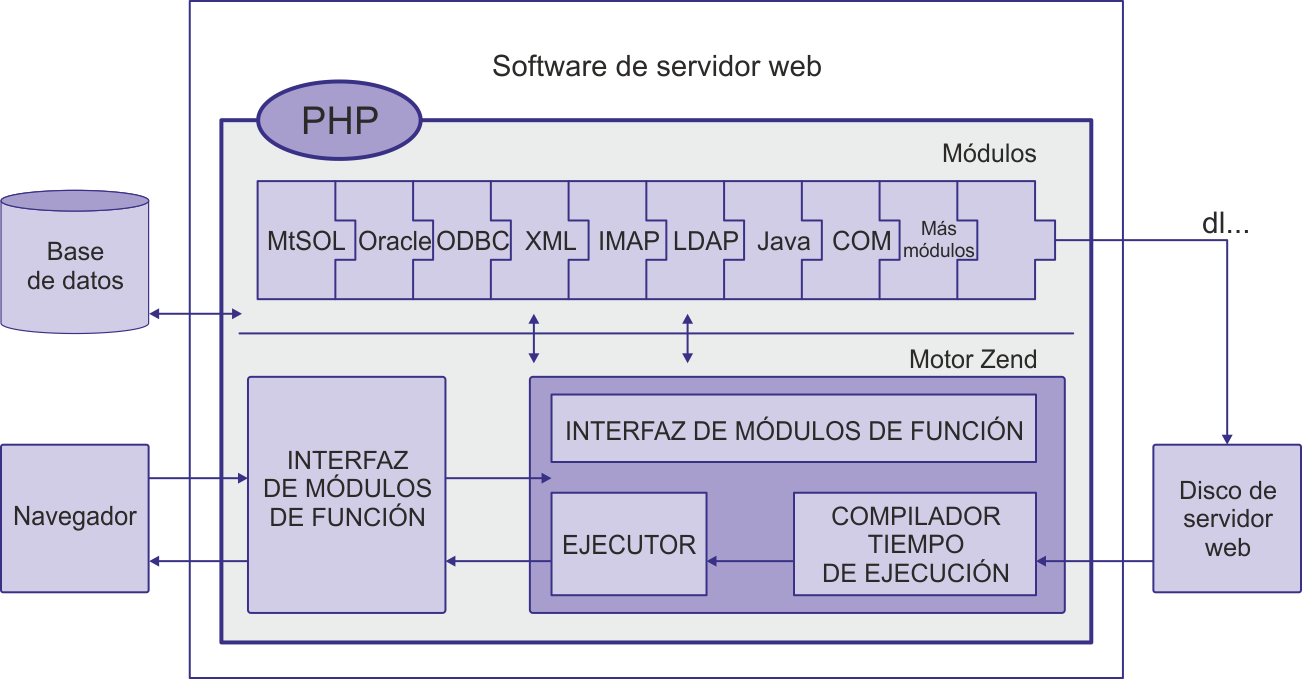
\includegraphics[width=0.8\textwidth]{imagenes/estructura_php.png}
    \label{fig:estructuraphp}
    \caption{Estructura interna de PHP}
\end{figure}



\subsection{HTML 5}[b]
HTML (Hyper Text Markup Language) es el lenguaje usado para escribir las páginas web, describe la estructura y el contenido usando solo texto y lo complementa con objetos tales como imágenes, flash y otros. Los archivos así creados son guardados con la extensión de archivo HTM o HTML.




Su estructura se compone de etiquetas o tags entre las cuales van insertados los diferentes elementos que componen la pagina como son los bloques de texto, scripts y la ruta a la ubicación de archivos externos como imágenes y otros archivos multimedia. El navegador al cargar dichos archivos representa todos los elementos en ella de forma adecuada.

Existen varias versiones o especificaciones de HTML, son las siguientes:
\begin{itemize}
    \item HTML la primera especificación de 1991.
    \item HTML 3.0 propuesta por el recién formado W3C en 1995.
    \item HTML 4 1999.
    \item XHTML 2002.
    \item HTML5 usándose actualmente pero aun en desarrollo.
\end{itemize}

\begin{figure}[hb]
    \centering
    
\includegraphics[width=0.3\textwidth]{imagenes/HTML5-Logo.png}
    \caption{Logo de HTML5}
    \label{fig:logoHTML}
\end{figure}

HTML5 surge como una evolución lógica de las especificaciones anteriores y por la necesidad de lograr los siguientes objetivos:
\begin{itemize}
    \item Lograr que la información, y la forma de presentarla estén lo más separadas posible.
    \item Resumir, simplificar y hacer más sencillo el código utilizado.
    \item Un lenguaje que haga las páginas compatibles con todos los navegadores web, incluyendo los de los teléfonos móviles y otros dispositivos modernos usados en la actualidad para navegar en Internet.
    \item Eliminar restricciones que hagan el código más popular y asequible.
\end{itemize}

\subsubsection{Principales estándares en el lenguaje HTML}

HTML4
Posiblemente el lenguaje mas usado en las paginas de Internet es el HTML4, a pesar de estar ya casi obsoleto debido a sus limitaciones.
Muchos CMS, están diseñados para crear las paginas usando dicha especificación, por lo que se siguen sumando muchas de ellas a los millones acumuladas en los servidores de Internet.
Una página escrita en HTML4 puede ser que se muestre de forma diferente en distintos navegadores, o que no se muestre en lo absoluto.
Es imposible representar en dicho lenguaje multitud de caracteres especiales como los Unicode, que son tan comunes en las páginas.

XHTML
Después del HTML4 surge el XHTML en dos versiones, Transitional y Strict, lenguaje desde sus inicio considerado de transición y de uso temporal, no obstante representa un adelanto enorme respecto a las posibilidades que introduce, limitado siempre al tratar de mantener la compatibilidad con la especificación anterior. 
Es más ligero y compatible con cualquier navegador, su desventaja es que posee muchas restricciones, por lo que muchos no se habituaron fácilmente al salto que representó su introducción y aun siguen atrapados en el lenguaje anterior.

HTML5
Finalmente llega HTML5, recoge todas las ventajas que introdujo el XHTML y elimina bastante restricciones y limitaciones.
Es más ligero al ser más sencillo y simple el código, lo que permite que las paginas escritas en este lenguaje carguen mas rápido en el navegador.
Si aun no fuera suficiente, introduce infinidad de opciones que hasta ahora estaban vedadas a las páginas web, como insertar directamente vídeo, música, y casi cualquier elemento.

\subsubsection{Novedades de HTML 5}

En términos de Markup, el HTML5 introduce algunos elementos que hacen que se adecue a los tiempos que corren. Así, muchas de las novedades están relacionadas con la forma de construir websites que se tiene en la actualidad. Una de las más importantes novedades está relacionada con la inserción de multimedia en los sitios web, que ahora contarán con etiquetas HTML especiales para poder ser incluidos. Por otro lado, algunos aspectos de diseño también son incluidos en el lenguaje, así como también algunos detalles de navegación.

Con el uso de HTML5, se puede reducir la dependencia de los plug-ins que tenemos que tener instalados para poder ver una determinada web. Caso emblemático, el de Adobe Flash, que se ve claramente perjudicado por la instauración de este estándar. Por otro lado, fue un avance importante para dispositivos que de forma nativa no soportaban Flash, y que no soportaban tampoco plug-ins necesarios para hacerlo. Pero además, con HTML5 se amplía el horizonte del desarrollo de aplicaciones que pueden ser usadas en una multiplicidad de dispositivos.

Gracias a HTML5, los usuarios pueden acceder a sitios web de manera offline, sin estar conectados a internet. Se suma también la funcionalidad de drag and drop, y también la edición online de documentos ampliamente popularizada por Google Docs. La geolocalización es uno de sus puntos fuertes, pero por otro lado, las etiquetas diseñadas especialmente para el audio y el vídeo ahorran la necesidad de tener que tener un plug-in.

\subsubsection{Las nuevas etiquetas}
El lenguaje HTML funciona a través de marcas de sentido llamadas etiquetas. Las etiquetas son la herramienta fundamental para que los navegadores puedan interpretar el código y permitirnos ver imágenes, texto, párrafo, y estructuras. Los navegadores vendrían a ser como “traductores” de las etiquetas, y con HTML5, se agregan nuevas etiquetas para utilizar que nos ahorran el uso de otros productos que se usaban para complementar y hacer cosas que con el simple HTML no se podían hacer. 

HTML5 fue creado para hacer que el proceso de escribir el código sea más simple y más lógico, por decirlo de una forma. La sintaxis de HTML5 se destaca, como dijimos, en el ámbito multimedia, pero son bastantes las etiquetas introducidas para generar una mejoría.

La idea detrás de HTML5 es que podamos visualizar el contenido multimedia variado que podemos encontrar en Internet aún cuando nos encontramos en dispositivos de gama baja que no podrían soportarlo. No solamente contamos con etiquetas especiales como audio, vídeo y canvas, sino también integración con contenidos de gráficos en vectores (que anteriormente se conocía como la etiqueta object). Con estas etiquetas, los usuarios pueden consumir vídeos y canciones, por ejemplo, sin necesidad de instalar nada de forma adicional.

Las más importantes de las nuevas etiquetas creadas son:

\begin{description}
    \item[article] esta etiqueta sirve para definir un artículo, un comentario de usuario o una publicación independiente dentro del sitio.
    \item[nav] la negación puede ser insertada directamente en el markup, entre estas etiquetas, que nos permitirán hacer que nuestras listas oficien de navegación.
    \item[section] con esta etiqueta, una de las más importantes de las novedades, se puede definir todo tipo de secciones dentro de un documento. Por ponerlo de forma sencilla, funciona de una forma similar a la etiqueta div que nos separa también diferentes secciones.
    \item[embed] con esta etiqueta se puede marcar la presencia de un contenido interactivo o aplicación externa.
    \item[header, footer] estas etiquetas individuales ahorran tener que insertar IDs para cada uno, como se solía hacer anteriormente. Además, se pueden insertar headers y footers para cada sección, en lugar de tener que hacerlo únicamente en general.
    \item[audio y video] estas son las dos más importantes etiquetas de HTML5, dado que nos permiten acceder de forma más simple a contenido multimedia que puede ser reproducido por casi todo tipo de dispositivos; marcan el tipo de contenido que estará en su interior.
    \item[canvas] finalmente, esta etiqueta nos permite introducir un “lienzo” dentro de un documento, para poder dibujar gráficos por vectores; será necesario el uso de JavaScript.
\end{description}

Hay otras etiquetas inauguradas por HTML5 pero destacamos estas por la innovación que introducen en nuestro código. 

Las etiquetas a las que estábamos acostumbrados, por otro lado, introducen un nuevo funcionamiento. El caso ejemplo es el de las etiquetas header y footer, que, como dijimos, ahora permiten separar las secciones, y no solamente el comienzo y el fin de una página.

El funcionamiento del DOCTYPE también se renueva, siendo mucho más simple de usar y menos engorroso. 

\subsection{CSS 3}

El CSS es un lenguaje de estilos empleado para definir la presentación, el formato y la apariencia de un documento de marcaje, sea html, xml, o cualquier otro. Comúnmente se emplea para dar formato visual a documentos html o xhtml que funcionan como espacios web. También puede ser empleado en formatos xml, u otros tipos de documentos de marcaje para la posterior generación de documentos.

\begin{figure}[htb]
    \centering
    
\includegraphics[width=0.3\textwidth]{imagenes/css3logo.png}
    \caption{Logo de CSS 3}
    \label{fig:logocss}
\end{figure}

Las hojas de estilos nacen de la necesidad de diseñar la información de tal manera que podemos separar el contenido de la presentación y, así, por una misma fuente de información, generalmente definida mediante un lenguaje de marcaje, ofrecer diferentes presentaciones en función de dispositivos, servicios, contextos o aplicativos. Por lo que un mismo documento html, mediante diferentes hojas de estilo, puede ser presentado por pantalla, por impresora, por lectores de voz o por tabletas braille. Separamos el contenido de la forma, composición, colores y fuentes.

La especificación de CSS está mantenida por el World Wide Web Consortium (W3Cg).


Las diferentes revisiones de las hojas de estilo tienen el origen en la primera especificación publicada por el W3C en diciembre de 1996 y que pretendía unificar la sintaxis y el modo de definir una hoja de estilos por los diferentes lenguajes derivados del SGML. Así, las principales características que se pueden definir mediante esta primera especificación son:
\begin{itemize}
    \item Propiedades del tipo de letra, así como el estilo de este.
    \item Colores de los textos y de los fondos.
    \item Atributos del texto tales como espacio entre caracteres, palabras y líneas.
    \item Alineación de tablas, bloques de texto, imágenes, párrafos.
    \item Márgenes externos e internos, filetes y posición de la mayoría de los elementos.
    \item Definición única de elementos mediante ids y agrupamiento de atributos
    mediante classes.
\end{itemize}

A partir de esta primera especificación, en mayo de 1998, y como una extensión a la primera revisión, aparece la segunda, popularmente conocida como la especificación CSS2, y adoptada por la mayoría de los navegadores. 

Como características fundamentales que añade la revisión, se encuentra la posibilidad de definir posiciones de forma absoluta, relativa y fija, así como la profundidad de los elementos (z-index) cuando existen superposiciones, también el soporte para formatos de voz y textos bidireccionales. De esta, aparece una revisión, la 2.1, que incorpora muchas de las mejoras hechas por los fabricantes de navegadores y que actualmente es empleada y estandarizada.

La tercera revisión de la especificación del CSS por el W3C empieza en el 2005 y todavía está en proceso de definición. Pero esta vez, las diferentes implementaciones de los motores de renderizado de los navegadores no están esperando a tener una especificación, sino que implementan ciertas cosas a su manera y, por lo tanto, muchas son utilizables en entornos de producción web. 

Es necesario, sin embargo, partir siempre de la consideración de que las diferentes implementaciones de los navegadores no es exacta, y de que, por lo tanto, cuando diseñamos una hoja de estilos, el principio que tiene que regir es que funcione en todas partes, y no que funcione igual.

A diferencia de las otras especificaciones, esta vez se ha dividido en temas. De este modo disponemos de diferentes temas que pueden crecer y evolucionar en paralelo, y no como uno grande y monolítico, con muchísimas revisiones (cada vez hay más gente interesada y evoluciona más deprisa).

Así, en la nueva revisión encontramos grupos como el de selectores, unidades de medida, modelo de caja, colores y gamas, modelo de línea, texto, fuentes, lenguajes verticales, page-media... entre otros. Y de este modo, diferentes módulos tienen un estatus diferente y son adoptados por los fabricantes de software a diferente velocidad.

A grandes rasgos podemos destacar dos beneficios del uso de CSS3
\begin{description}
    \item[Reducción del tiempo de desarrollo y mantenimiento] Utilizar propiedades y métodos de CSS3 puede ser un beneficio directo a la hora
    de desarrollar, puesto que nos ahorramos bastante trabajo, como por ejemplo
    a la hora de hacer fondo con esquinas redondeadas. Antes había que hacerlo
    con imágenes. También ahorramos mucho trabajo a la hora de hacer
    sombras, ya que nos ahorramos de nuevo la imagen que teníamos que usar
    antes (normalmente un gráfico en formato png).
    También podemos mejorar el rendimiento al tener menos código, divs dentro
    de divs, etc.
    \item[Incremento del rendimiento de las páginas] Menos etiquetas html indican\\ menos código a la hora de descargarse del servidor  y menos código a la hora de interpretar y dibujar el navegador. Dos ahorros, uno de ancho de banda y el otro de rendimiento del ordenador. Además, muchas de las técnicas de CSS3 nos ahorran imágenes, que a la vez cumplen la doble premisa de rendimiento.
\end{description}



Las novedades de CSS3 con respecto a las versiones anteriores incluyen:
\begin{description}
    \item[Nuevos selectores] Los selectores CSS son la herramienta más potente del lenguaje de estilos, puesto que nos permiten seleccionar diferentes elementos del contenido html en función de la etiqueta o de sus atributos sin tener que hacer uso de su clase, su ID o Javascript.
    \begin{itemize}
        \item Selectores de atributos.
        \item Pseudo-clases.
        \item Pseudo-elementos.
        \item ...
    \end{itemize}
    
    \item[Colores RGBA] La posibilidad de especificar colores en modo RGB ya existía desde la especificación 2, pero en la versión 3 se ve ampliada con un nuevo modelo de color, el basado en saturación (HSL), y la posibilidad de especificar canal alpha sobre
    los colores.
    
    \item[Colores HSL] El modelo de color HSL (hue, saturation, light), tono, saturación y luz; define el color a partir de estos tres parámetros. Así, para una tonalidad de color dada, podemos alterar la saturación a partir del segundo parámetro, y la cantidad de  luz en el tercer parámetro.
    
    \item[Opacidad] Como su nombre indica, la opacidad nos permite definir el nivel de transparencia para un selector. A diferencia del modelo RGB, la transparencia se aplica
    al objeto y todos sus hijos y/o contenidos.
    
    \item[Esquinas redondeadas] Seguramente es la propiedad CSS3 más esperada y deseada por los diseñadores html. Permite redondear las esquinas de una caja (div, span... ) dado un radio, sin la necesidad de usar nada más.
    
    \item[Sombras, en cajas y texto] En la versión 2 de la especificación se introdujo la posibilidad de generar sombras directamente desde código CSS, pero se quitó en la 2.1 y se ha vuelto a introducir en la versión 3.
    
    \item[Webfonts] Otra de las posibilidades que resulta muy atractiva a la hora de emplear los CSS3 es la capacidad de adjuntar tipografías a un documento html. A partir de la especificación 3, disponemos de la etiqueta @font-face, que nos permite definir una tipografía.
    
    \item[MediaQueries] Desde la versión 2.1 de los CSS, existe la posibilidad de definir estilos en función del uso de la hoja: una para la pantalla (screen), otra para la impresión (print), otra para los lectores de voz (voice). A partir de la especificación 3 esto va un paso más allá, y nos permite definir estilos específicos para diferentes tamaños de pantalla. La posibilidad de poder trabajar así, realmente, nos ofrece soluciones óptimas, puesto que podemos emplear sólo CSS para crear una versión móvil de un site.
\end{description}


\subsection{Javascript}

Javascript es un lenguaje de programación que surgió con el objetivo inicial de programar ciertos comportamientos sobre las páginas web, respondiendo a la interacción del usuario y la realización de automatismos sencillos. En ese contexto podríamos decir que nació como un <<lenguaje de scripting>> del lado del cliente, sin embargo, hoy Javascript es mucho más. Las necesidades de las aplicaciones web modernas y el HTML5 ha provocado que el uso de Javascript que encontramos hoy haya llegado a unos niveles de complejidad y prestaciones tan grandes como otros lenguajes de primer nivel.

Pero además, en los últimos años Javascript se está convirtiendo también en el lenguaje <<integrador>>. Lo encontramos en muchos ámbitos, ya no solo en Internet y la Web, también es nativo en sistemas operativos para ordenadores y dispositivos, del lado del servidor y del cliente. La visión de Javascript <<como lenguaje para crear pequeños programas dentro del ámbito de una página web>> se ha quedado muy pequeña.

En el contexto de un sitio web, con Javascript se puede hacer todo tipo de acciones e interacción. Antes se utilizaba para validar formularios, mostrar cajas de diálogo y poco más. Hoy es el motor de las aplicaciones más conocidas en el ámbito de Internet: Google, Facebook, Twitter, Outlook...

A Javascript se le denomina <<del lado del cliente>> porque donde se ejecuta es en el navegador (cliente web), en contraposición a lenguajes como PHP que se ejecutan del <<lado del servidor>>. 

En Javascript, es el navegador el que soporta la carga de procesamiento. Gracias a su compatibilidad con todos los navegadores modernos se ha convertido en un estándar como lenguaje de programación del lado del cliente.

Con Javascript podemos crear y definir interacciones con el usuario. El navegador del cliente es el encargado de interpretar las instrucciones Javascript y ejecutarlas para realizar estas interactividades, de modo que el mayor recurso, con que cuenta este lenguaje es el propio navegador y todos los elementos que hay dentro de una página. Pero ahora, gracias a las API Javascript de HTML5, que están disponibles en los navegadores actuales de ordenadores y dispositivos, podemos acceder a todo tipo de recursos adicionales, como la cámara, espacio para almacenamiento de datos, creación de gráficos basados en vectores y mapas de bits, flujos de datos con servidores, etc. Con todo ello se han multiplicado las posibilidades.


JavaScript es un lenguaje de programación interpretado, dialecto del estándar ECMAScript. Se define como orientado a objetos, basado en prototipos, imperativo, débilmente tipado y dinámico.

JavaScript se diseñó con una sintaxis similar al C, aunque adopta nombres y convenciones del lenguaje de programación Java. Sin embargo Java y JavaScript no están relacionados y tienen semánticas y propósitos diferentes.

Las propiedades más importantes de JavaScript son las siguientes:
\begin{itemize}
    \item Se interpreta por el ordenador que recibe el programa, no se compila.
    \item Tiene una programación orientada a objetos. El código de los objetos está predefinido y esexpandible. No usa clases ni herencia.
    \item El código está integrado (incluido) en los documentos HTML.
    \item Trabaja con los elementos del HTML.
    \item No se declaran los tipos de variables.
    \item Ejecución dinámica: los programas y funciones no se chequean hasta que se ejecutan.
    \item Es orientado a eventos, los programas se ejecutan cuando sucede algo, un evento.
\end{itemize}

La sintaxis de JavaScript es muy similar a la de otros lenguajes de programación como Java y C. Las normas básicas que definen la sintaxis de JavaScript son las siguientes:
\begin{description}
    \item[No se tienen en cuenta los espacios en blanco y nuevas líneas] Como sucede con XHTML, el intérprete de JavaScript ignora cualquier espacio en blanco sobrante, por lo que el código se puede ordenar de forma adecuada para entenderlo mejor (tabulando las líneas, añadiendo espacios, creando nuevas líneas, etc...)
    
    \item[Se distinguen las mayúsculas y minúsculas] Al igual que sucede con la sintaxis de las etiquetas y elementos XHTML. Sin embargo, si en una página XHTML se utilizan indistintamente mayúsculas y minúsculas, la página se visualiza correctamente, siendo el único problema la no validación de la página. En cambio, si en JavaScript se intercambian mayúsculas y minúsculas el script no funciona.
    
    \item[No se define el tipo de las variables] Al crear una variable, no es necesario indicar el tipo de dato que almacenará. De esta forma, una misma variable puede almacenar diferentes tipos de datos durante la ejecución del script.
    
    \item[No es necesario terminar cada sentencia con el carácter ;] En la mayoría de lenguajes de programación, es obligatorio terminar cada sentencia con el carácter ;. 
        
    \item[Se pueden incluir comentarios] Los comentarios se utilizan para añadir información en el código fuente del programa. Aunque el contenido de los comentarios no se visualiza por pantalla, si que se envía al navegador del usuario junto con el resto del script, por lo que es necesario extremar las precauciones sobre la información incluida en los comentarios.
\end{description}

\section{Frameworks}

El concepto framework se emplea un muchos ámbitos del desarrollo de sistemas software, no solo en el ámbito de aplicaciones Web. Podemos encontrar frameworks para el desarrollo de aplicaciones médicas, de visión por computador, para el desarrollo de juegos, y para cualquier ámbito que pueda ocurrírsenos.

En general, con el término framework, nos estamos refiriendo a una estructura software compuesta de componentes personalizables e intercambiables para el desarrollo de una aplicación. En otras palabras, un framework se puede considerar como una aplicación genérica incompleta y configurable a la que podemos añadirle las últimas piezas para construir una aplicación concreta. 

Los objetivos principales que persigue un framework son: acelerar el proceso de desarrollo, reutilizar código ya existente y promover buenas prácticas de desarrollo como el uso de patrones.

El objetivo principal de todo framework es facilitar las cosas a la hora de desarrollar una aplicación, haciendo que nos centremos en el verdadero problema y nos olvidemos de implementar funcionalidades que son de uso común.

El uso de un framework a la hora de realizar un proyecto, ofrece importantes ventajas, ventajas ya no sólo al facilitarnos la tarea de la creación de la aplicación, sino otras como en el mantenimiento del código, realizar ampliaciones, etc...

Otras ventajas son:
\begin{description}
    \item[Uso de patrones de diseño] Uno de las principales ventajas que ofrecen los framework es el uso de patrones de diseño para el desarrollo de la aplicación. El patrón más utilizado y que casi todos los framework utilizan es el conocido como Modelo – Vista – Controlador (MVC).
    
    \item[Estructura predefinida de la aplicación] El programador no necesita plantearse la estructura global de la aplicación, ya que esta es proporcionada por el  framework. Tiene la ventaja de que pasado un tiempo, si hay  que tocar algo en la aplicación, sabremos donde encontrar el archivo en cuestión de forma rápida.
    
    \item[Código altamente testeado] Todo el código que forma parte del framework está altamente probado, lo que garantiza el buen    funcionamiento del mismo. Se podría desarrollar esas mismas funcionalidades, pero   nunca podremos garantizar el nivel de testeo que ofrece un framework.
    
    \item[Comunidad de usuarios detrás de cada framework] La gran mayoría de los frameworks tienen detrás a una amplia comunidad de usuarios, de los    cuales muchos ayudan en su desarrollo o creando extensiones con funcionalidades extra que podremos utilizar de forma sencilla sin tener que desarrollarlas por nuestra cuenta.
\end{description}

\subsubsection{Patrón MVC, Modelo Vista Controlador}

Para comprender como trabajan los frameworks Web existentes es imprescindible conocer el patrón MVC.

El patrón Modelo-Vista-Controlador es una guía para el diseño de arquitecturas de aplicaciones que ofrezcan una fuerte interactividad con usuarios. Este patrón organiza la aplicación en tres modelos separados, el primero es un modelo que representa los datos de la aplicación y sus reglas de negocio, el segundo es un conjunto de vistas que representa los formularios de entrada y salida de información, el tercero es un conjunto de controladores que procesa las peticiones de los usuarios y controla el flujo de ejecución del sistema.

El modelo MVC puede ser implementado sin la necesidad de utilizar un framework, pero la diferencia radica en que el framework nos obliga a utilizarlo, creando de esta forma un código mucho más robusto. 

Además el uso de este tipo de utilidades nos ayuda a evitar el conocido como <<código spaghetti>>, que consiste en meter funcionalidades en capas que no corresponde, lo que con el paso de tiempo hará que nuestro código sea un verdadero caos.

La mayoría, por no decir todos, de los framewroks para Web implementan este patrón. 


Algunas caracteristicas presentes en casi todos los frameworks web son:
\begin{description}
    \item[Abstracción de URLs y sesiones] No es necesario manipular directamente las URLs ni las sesiones, el framework ya se encarga de hacerlo. 
    
    \item[Acceso a datos] Incluyen las herramientas e interfaces necesarias para     integrarse con herramientas de acceso a datos, en BBDD,
    XML, etc... 
    
    \item[Controladores] La mayoría de frameworks implementa una serie de     controladores para gestionar eventos, como una     introducción de datos mediante un formulario o el acceso a     una página. Estos controladores suelen ser fácilmente     adaptables a las necesidades de un proyecto concreto. 
    
    \item[Autentificación y control de acceso] Incluyen mecanismos para la identificación de usuarios mediante login y password y permiten restringir el acceso a     determinas páginas a determinados usuarios. 
   
    \item[Internacionalización]
    
    \item[Separación entre diseño y
    contenido]
\end{description}

En la realización de este proyecto se ha incorporado diversos frameworks. Principalmente dos:
\begin{itemize}
    \item Laravel, para PHP.
    \item Bootstrap, para CSS.
\end{itemize}

\subsection{Laravel}
Durante varios años PHP se ha ganado una mala reputación entre los desarrolladores que tuvieron que mantener aplicaciones desarrolladas sin ningún tipo de estructuración.

Pasó el tiempo y apareció el proyecto Symfony, el cual está basado en los principios de crear un desarrollo más sólido flexible y testeable, algo que las aplicaciones PHP no tenían.

Laravel nace confiando en Symfony, pero también depende de otras grandes librerías como SwiftMailer, Carbon o Doctrine, es decir, se ha tomado la mejor de los grandes para hacer un framework muy robusto.

Laravel se apoya en las mejoras introducidas en las últimas versiones de PHP como pueden ser:
\begin{description}
    \item[Espacios de nombres (namespaces)] Se utilizan extensivamente en lenguajes como Java y evitan la colisión de nombres cuando el mismo nombre de función se utiliza en diferentes librerías. Los espacios de nombres se separan mediante “\\”, y éstos se deben replicar en la estructura del directorio. Se declaran en la parte superior del archivo tomando una estructura como . 
    \begin{verbatim}
        <?php 
        namespace Illuminate\Database\Eloquent
        ?>
    \end{verbatim}
    Para indicar los espacios de nombres en los que PHP deberá buscar las clases, utilizamos la palabra “use” seguida del espacio de nombre de la clase, por ejemplo: \verb|use Illuminate\Database\Eloquent\Model|.
    \item[Interfaces (interfaces)]  También se conocen como Contratos y son una forma de definir los métodos que una clase deberá proveer, si implementa esa interfaz. Las Interfaces no contiene ningún detalle de implementación, únicamente son contratos.
    
    \item[Funciones anónimas] Ayudan a crear código más corto y se utilizan para definir rutas, eventos, filtros y en otras partes. Ejemplo de una función anónima en una ruta: \verb|Route::get(‘hi’, function(){ return ‘hi’;});|
    
    \item[Sobrecarga (overloading)] También llamados métodos dinámicos o mágicos, nos permiten llamar a métodos que no estaban previamente definidos en una clase. Ejemplo: \verb|whereUsernameOrEmail ($name, $email)|.  
    
    Estas llamadas se manejan con el método \verb| _call()|, el cual trata de pasear el nombre para ejecutar uno o más de los métodos conocidos. En este caso \verb|->where(‘usuario’, $usuario)->orWhere(‘email’,$email)|.


\end{description}

\begin{figure}[htb]
    \centering
    
\includegraphics[width=0.8\textwidth]{imagenes/laravel-logo.png}
    \caption{Logo de Laravel}
    \label{fig:logolaravel}
\end{figure}

Laravel: Principales características y fuentes de inspiración

\subsubsection{Principales características}

Veamos qué es lo que se puede esperar de un proyecto con Laravel y como éstas características pueden ayudar a incrementar la productividad:

\begin{description}
    \item[Modularidad] Laravel se ha construido utilizando más de 20 librerías diferentes fuertemente integradas con el gestor de dependencias Composer.
    
    \item[Testeabilidad] Construido para facilitar el testeo, Laravel tiene con varios asistentes (helpers) que ayudan a visitar las rutas de testeo, navegando por el HTML resultante para asegurar que los métodos que se llaman desde las diferentes clases sean correctos, e incluso a impersonar a los usuarios.
    
    \item[Enrutamiento (routing)] Laravel proporciona un extrema flexibilidad en la definición de las rutas de la aplicación. Inspirado en la filosofía de los micro-frameworks Sinatra y Silex. Todavía más, es posible adjuntar funciones de filtro que se ejecuten en rutas específicas.
    
    \item[Gestor de configuración] Frecuentemente la aplicación se ejecutará en diferentes entornos, esto quiere decir que tanto la base de datos como credenciales o dominios serán diferentes si se ejecutan el local en el entorno de test o en los servidores de producción. Laravel nos permite definir configuraciones separadas para cada uno de los entornos.
    
    \item[Confeccionador de consultas y ORM] Cuando se instala Laravel viene con un constructor de consultas, este nos permite lanzar consultas a la base de datos con una sintaxis PHP de métodos enlazados, en lugar de tener que escribir la SQL completa. Además proporciona un ORM y una implementación de RegistroActivo (ActiveRecord) llamado Eloquent, que permite definir modelos interconectados. Estos componentes son compatibles con bases de datos tales como PostgreSQL, SQLite, MySql, MS SQL Server.
    
    \item[Confeccionador esquema, migraciones y repoblaciones] Inspirado por la filosofía Rails, estas características permiten definir un esquema de base de datos dentro de PHP y mantener un registro de los cambios para así ayudar en la migración de base de datos. Las repoblaciones (Seeding) permiten poblar las tablas seleccionadas de una base de datos una vez realizada la migración para de esta forma rellenar con datos las tablas.
    
    \item[Motor de plantillas] Laravel viene con Blade, un lenguaje ligero de plantillas con el cual se pueden crear diseños anidados con bloques predefinidos en el que el contenido se inserta dinámicamente. Además Blade guarda en caché los archivos generados.
    
    \item[Autenticación] Laravel viene con las herramientas para crear en toda web un formulario de registro, autenticación e incluso envio de contraseñas a usuarios que no la recuerden.
    
    \item[Redis] Es un sistema de almacenamiento clave-valor en memoria que tiene fama de ser extremadamente rápido.
    \item[Colas] Laravel se integra con diversos servicios de colas, tales como Amazon SQS o IronMQ, para permitir el aplazamiento de tareas que son muy intensivas en recursos, así por ejemplo podemos enviar una gran cantidad de e-mails ejecutando esta tarea en segundo plano en lugar de hacer que el usuario espere delante de la pantalla.
\end{description}

\subsubsection{Simplicidad en la sintaxis}

El corazón de la filosofía de Laravel es la simplicidad y la expresividad. Esto quiere decir que los desarrolladores de Laravel han dado especial atención en el nombrado de las clases para comunicar con efectividad las acciones en un inglés sencillo.

Observemos el siguente trozo de código:

\begin{verbatim}

<? php
Route:: get(' area/{ id}', function( $ id){
    if( 51 = = $ area and !Auth:: check()) {
        return Redirect:: guest(' login');
    } else {
    return “Bienvenido a tu parte ”. $area;
}
})->where (‘id’,’[0-9]+’);

\end{verbatim}

A simple vista nos podemos  hacer una idea de lo que  hace este código. Eso es expresividad, hacer que el código sea más legible, con lo que probablemente también será  un codigo más sencillo y menos propenso a errores.




\subsection{Bootstrap}

Twitter Bootstrap es un framework o conjunto de herramientas de software para diseño de sitios y aplicaciones web. Contiene plantillas de diseño con tipografía, formularios, botones, cuadros, menús de navegación y otros elementos de diseño basado en HTML y CSS, así como, extensiones de JavaScript opcionales adicionales.

Es el proyecto más popular en GitHub y es usado por la NASA y la MSNBC junto a más organizaciones.

Bootstrap fue desarrollado por Mark Otto y Jacbod Thornton de Twitter, como framework para fomentar la consistencia a través de herramientas internas. Antes de Bootstrap, se usaban varias librerías para el desarrollo de interfaces de usuario, las cuales guiaban a inconsistencias y a una carga de trabajo alta en su mantenimiento. 

Según el desarrollador de Twitter Mark Otto, frente a esos desafíos:
\begin{quotation}
    ...un pequeño grupo de desarrolladores y yo nos reunimos a diseñar y construir una nueva herramienta interna y vimos una oportunidad de hacer más. A través de ese proceso, nos vimos construir algo mucho más sustancial que otra herramienta interna más. Meses después, terminamos con una primera versión de Bootstrap como una manera de documentar y compartir bienes y patrones de diseño comunes dentro de la compañía.
\end{quotation}

En agosto del 2011, Twitter liberó a Bootstrap como código abierto.


\subsubsection{Características}
Bootstrap tiene un soporte relativamente incompleto para HTML5 y CSS 3, pero es compatible con la mayoría de los navegadores web. La información básica de compatibilidad de sitios web o aplicaciones esta disponible para todos los dispositivos y navegadores. Existe un concepto de compatibilidad parcial que hace disponible la información básica de un sitio web para todos los dispositivos y navegadores. Por ejemplo, las propiedades introducidas en CSS3 para las esquinas redondeadas, gradientes y sombras son usadas por Bootstrap a pesar de la falta de soporte de navegadores antiguos. Esto extiende la funcionalidad de la herramienta, pero no es requerida para su uso.

Desde la versión 2.0 también soporta diseños responsables. Esto significa que el diseño gráfico de la página se ajusta dinámicamente, tomando en cuenta las características del dispositivo usado (PCs, tabletas, teléfonos móviles).


Bootstrap viene con una disposición de cuadricula estándar de 940 píxeles de ancho para posicionar los elementos de la aplicacion o pagina web. Aparte, también tiene cuatro variaciones para hacer uso de distintas resoluciones y tipos de dispositivos: teléfonos móviles(formato vertical y apaisado), tabletas y computadoras con baja y alta resolución. Esto ajusta el ancho de las columnas automáticamente.

También proporciona un conjunto de definiciones básicas de estilo para todos los componentes de HTML. Esto otorga uniformidad al visualizar la aplicacion en cualquier navegador y sistema.

Como añadido a los elementos principales de HTML, Bootstrap contiene otra interfaz de elementos comúnmente usados. Ésta incluye botones con características avanzadas (e.g grupo de botones o botones con opción de menú desplegable, listas de navegación, etiquetas horizontales y verticales, ruta de navegación, paginación, etc.), etiquetas, capacidades avanzadas de miniaturas tipográficas, formatos para mensajes de alerta y barras de progreso.

Los componentes de JavaScript para Bootstrap están basados en la librería jQuery de JavaScript. Los plug-ins proveen elementos adicionales de interfaz de usuario como diálogos, tooltips y carruseles. También extienden la funcionalidad de algunos elementos de interfaz existentes, incluyendo, por ejemplo, una función de auto-completar para campos de entrada (input). 

\subsubsection{Estructura y Función}
Bootstrap es modular y consiste esencialmente en una serie de hojas de estilo LESS que implementan la variedad de componentes de la herramienta. Una hoja de estilo llamada bootstrap.less incluye los componentes de las hojas de estilo. Los desarrolladores pueden adaptar el mismo archivo de Bootstrap, seleccionando los componentes que deseen usar en su proyecto.

Los ajustes son posibles en una medida limitada a través de una hoja de estilo de configuración central. Los cambios más profundos son posibles mediante las declaraciones LESS.

El uso del lenguaje de hojas de estilo LESS permite el uso de variables, funciones y operadores, selectores anidados, así como clases mixins.

Desde la versión 2.0, la configuración de Bootstrap también tiene una opción especial de <<Personalizar>> en la documentación. Por otra parte, los desarrolladores eligen en un formulario los componentes y ajustes deseados, y de ser necesario, los valores de varias opciones a sus necesidades. El paquete consecuentemente generado ya incluye la hoja de estilo CSS pre-compilada.

















    \chapter{Implementación}
 \section{Objetivos}
 El objetivo general de este proyecto es acercar la domótica, y los beneficios que ello conlleva, a hogares con menos recursos. Romper la barrera de que estos sistemas son un lujo, y pasen a ser algo cotidiano y al alcance de todos.
 
  Conseguir este objetivo es algo muy ambicioso, aún así, para dejar nuestro granito de arena en este largo camino, 
  intentaremos crear un sistema de bajo coste. Basado en elementos de uso común en  electrónica y en el equipamiento habitual en las viviendas actuales.  Para ello nos proponemos dos objetivos concretos.
  
  El primer objetivo es crear un marco de trabajo y de comunicaciones entre los distintos elementos, para que estos puedan trabajar al unísono y en armonía, y sirva de base para poder implementar las funciones de un sistema domótico.
  
  El segundo objetivo es implementar  un sistema domótico propio sobre la base anterior. Este sistema servirá tanto como demostración practica de la funcionalidad del sistema, como un primer módulo del sistema que pretendemos construir.
  
  Como vimos anteriormente, un sistema domótico es capaz de manejar muchos aspectos de la vida cotidiana de un hogar, éstas pueden ser alarmas de seguridad, incendios o escape de gases; automatización de persianas y toldos, control de luminarias, apertura y cierre de puertas, y un largo etcétera. 
  
  A causa de las limitaciones en tiempo y presupuesto, restringiremos las funciones del sistema al control de las luminarias y la monitorización de la temperatura.

\section{Escenario}
Para el desarrollo del proyecto necesitamos partir de una base, un escenario concreto sobre el que construir el sistema. Este debe ser lo suficientemente amplio para que una vez acabado podamos extrapolar el sistema domótico al máximo de casos en la vida real.

Para ello, el escenario elegido es una vivienda unifamiliar ya construida y habitada. Ya que así, abarcamos  un gran conjunto de público que podría beneficiarse de la domótica, a la vez que es facilmente adaptable a viviendas en fase de construcción.


El escenario quedaría constituido de la siguiente forma:
\begin{description}
    \item[Lugar físico] Vivienda unifamiliar construida y habitada.
        \begin{itemize}
            \item Cableado de la instalacion eléctrica ya existente.
            \item Mezcla heterogénea de luminarias(bombillas de bajo consumo, halógenas, fluorescentes, etc...).
            \item Red doméstica instalada.
        \end{itemize}
    \item[Funciones del sistema] Limitado a las luminarias.
        \begin{itemize}
            \item Control On/Off.
            \item Deteccion de movimiento en zonas de paso y baños.
            \item Control de Escenas.
            \item Apagado General.
            \item Programación periódica de acciones.
            \item Monitorización de la temperatura.
        \end{itemize}
\end{description}

Una vez situados, pasaremos a describir la implementacion del sistema.


\section{Arquitectura}
El punto central del sistema es la Raspberry Pi. Ésta actúa como estación base o gateway de la red de sensores, y a la vez, está conectada a la red doméstica para servir la aplicación de usuario. Desde aquí se envian y reciben los comandos de la red de sensores, se reciben y traducen en comandos las ordenes del usuario, y se ejecutan las tareas periódicas del sistema. 


La red de sensores esta formada por placas arduino, una por cada habitación. Cada arduino esta al cargo de encender o apagar las luces de su habitacion, monitorizar la temperatura, ejecutar las ordenes recibidas desde la Raspberry y enviar a ésta la informacion pertinente del sistema.

La aplicación de usuario es una aplicación web, servida desde la Raspberry, que funciona como punto de entrada del usuario al sistema. Desde aquí es posible encender y apagar las luces, gestionar las escenas y programar acciones del sistema.

Desde el punto de vista del software, el sistema se compone tres capas. Éstas, en orden ascendente en nivel de abstracción, son: la programación de los nodos, un servidor central engargado de las comunicaciones y la gestión, y la aplicacion de usuario. Las dos últimas se ejecutan dentro de la Raspberry.

\section{Comunicaciones Raspberry Pi-Red de sensores}
Para las comunicaciones entre la Raspberry y la red de sensores hemos creado un pequeño protocolo basado en mensajes, encima del protocolo XBee. 

La red de sensores esta configurada en  malla para asegurar la interconexión de todos los nodos. Ya que en una vivienda, al haber numerosas paredes y obstáculos, con otras configuraciones podrían quedar zonas oscuras en la conexion a la red.

Dentro del protocolo XBee, los nodos de la red envian exclusivamente hacia la Raspberry; y ésta envía exclusivamente en broadcast. Además, los módulos estan configurados en <<modo transparente>>, esto es que todo lo que recibe por la patilla de envio, aparece en la patilla de recepción en el otro lado, de forma totalmente transparente. Con lo que a efectos de programación, solo vemos un puerto serie. 

También marcaremos los módulos XBee como routers de la red, para que esta que configurada en malla, así, aseguramos la interconexión de todos los nodos. Ya que en una vivienda, al haber numerosas paredes y obstáculos, con otras configuraciones podrían quedar zonas oscuras en la conexion a la red.


Usar el protocolo XBee como base del nuestro nos proporciona algunas ventajas. Es inalámbrico, con lo que ahorramos en instalación de cables. Y podemos olvidarnos de los detalles como empaquetado, direccionamiento, colisiones, etc; que dejamos en manos de XBee, y centrarnos en enviar y recibir la información realmente importante para nosotros.

\subsection{Mensajes}
Como acabamos de ver, para los dispositivos de la red lo único que ven, en cuanto a comunicaciones,  es un puerto serie. Por lo que las comunicaciones tenemos que hacerlas en base a caracteres. 
 

Al fijar en el protocolo XBee el destino de los paquetes, necesitamos  direccionar nuestros mensajes. Tanto para que un nodo sepan si el mensaje es para el o no, como para que la Raspberry sepa de que nodo es el mensaje que le llega. Para ello, aprovecharemos el direccionamiento de los XBee, en nuestro protocolo cada nodo tiene un identificador, igual que su identificador en la red XBee.Además, reservaremos el identificador <<00>> para mensajes en broadcast.

Así pues, definimos el formato de los mensajes de la siguiente manera:

\begin{table}[h]
    \centering
    \begin{tabular}{cccc}
        \toprule
        MY & FUNCION & POSICION & VALOR \\ \toprule
        xx & xx      & xx       & xxx  \\ \bottomrule
    \end{tabular}
    \caption{Formato mensajes}
    \label{tab:formatoMensajes}
\end{table}


\begin{description}
    \item[MY] Es la identificación del nodo dentro de la red. Usamos la misma nomenclatura que en XBee para no sobrecargar de parámetros al usuario. Dos caracteres.
    \item[Función] Codigo de la función a ejecutar o de la que se está reportando. Dos caracteres, tipo entero.
    \item[Posición] Este campo hace referencia al actuador o sensor al que va dirigida la función. Dos caracteres, tipo entero.
    \item[Valor] Este campo se utiliza para comunicar el valor que toma, o debe tomar el actuador o sensor en cuestión. Tres caracteres, tipo entero.
\end{description}

Para facilitar las tareas de depuración y decodificación a los usuarios finales, decidimos optar por mensajes son de longitud fija.

Otra caracteristica de nuestro protocolo es que la  comunicación de datos es en base a unas funciones predefinidas en el sistema. Además, dependiendo de quien reciba el mensaje, este tiene un significado u otro.

Por el momento, las funciones definidas en el sistema son:

\begin{description}
    \item[Función <<00>>] Es el comando de una de las acciones especiales del sistema. Con este mensaje se apagan todas las luces de la vivienda.
    \item[Función <<10>>] Se usa para establecer el valor de un actuador, si el mensaje lo envia la Raspberry; o para informar de que un actuador ha cambiado de valor (por acción de un interruptor por ejemplo) si el que envia el mensaje es arduino.
    \item[Función <<20>>] la usamos tanto para pedir una temperatura, como para reportarla.
\end{description}

En la tabla \ref{tab:funcSistema} podemos ver el conjunto de funciones del sistema junto a un mensaje de red de ejemplo.


\begin{table}[h]
    \centering
    \begin{tabular}{cccp{6cm}}
        
        Función & Mensaje   & Destino & Descripción     \\ \toprule
        00      & 00 00- - - - -& Arduino & Apagar todo, mensaje en broadcast, establecer a 0 el valor de todos los actuadores \\ \midrule
        10      & mm10xxvvv & Arduino & Nodo con id mm, establecer valor vvv en actuador xx\\ \midrule
        10      & mm10xxvvv & Raspberry & El actuador xx del nodo mm tiene ahora el valor vvv \\ \midrule
        20      & mm20- - - - - & Arduino &  Petición de temperatura al nodo mm \\ \midrule
        20      & mm20- -vvv & Raspberry &  La temperatura *10 en el nodo mm es vvv \\ \midrule            
    \end{tabular}
    \caption{Funciones y mensajes del sistema}
    \label{tab:funcSistema}
\end{table} 



\section{Nodos - Arduino}
\subsection{Ubicación}
Para aprovechar los conductos del cableado eléctrico existente, hemos optado por ubicar un nodo de la red en cada habitacion de la vivienda. De esta manera, introducir los cables necesarios es mas sencillo, puesto que todo queda dentro de cada habitacion, que ya dispone de los conductos necesarios.

 Además, hace al sistema mas modulable al poder incorporar las habitaciones poco a poco.

\subsection{Equipamiento}
Cada nodo de la red esta equipado con:
\begin{itemize}
    \item Arduino UNO.
    \item Shield XBee.
    \item Sensor de temperatura.
    \item Sensor de presencia(opcional).
    \item Sensor de luz(opcional).
\end{itemize}

El sensor de temperatura lo usamos para monitorizar la temperatura de la vivienda, y en un futuro controlar la climatización. 

El sensor de presencia en conjunto con el sensor de luz se usan para el encendido automático de luces que por lo general solo se encienden un corto periodo de tiempo, por ejemplo, la luz de un pasillo.

\subsection{Cableado y conexiones}
 Para poder permitir que los nodos puedan interactuar con la vivienda es necesario introducir algunos cambios a esta.
 
 El primer cambio es convertir los interruptores que haya instalados en sensores para el nodo. Esto es tan sencillo como llevar dos cables desde el nodo al interruptor, uno conectado a tierra y el otro en cualquiera de las entradas digitales del arduino. En la figura \ref{fig:conexion-ard-int} se puede ver el esquema de la conexión.
 
 \begin{figure}[htb]
     \centering
     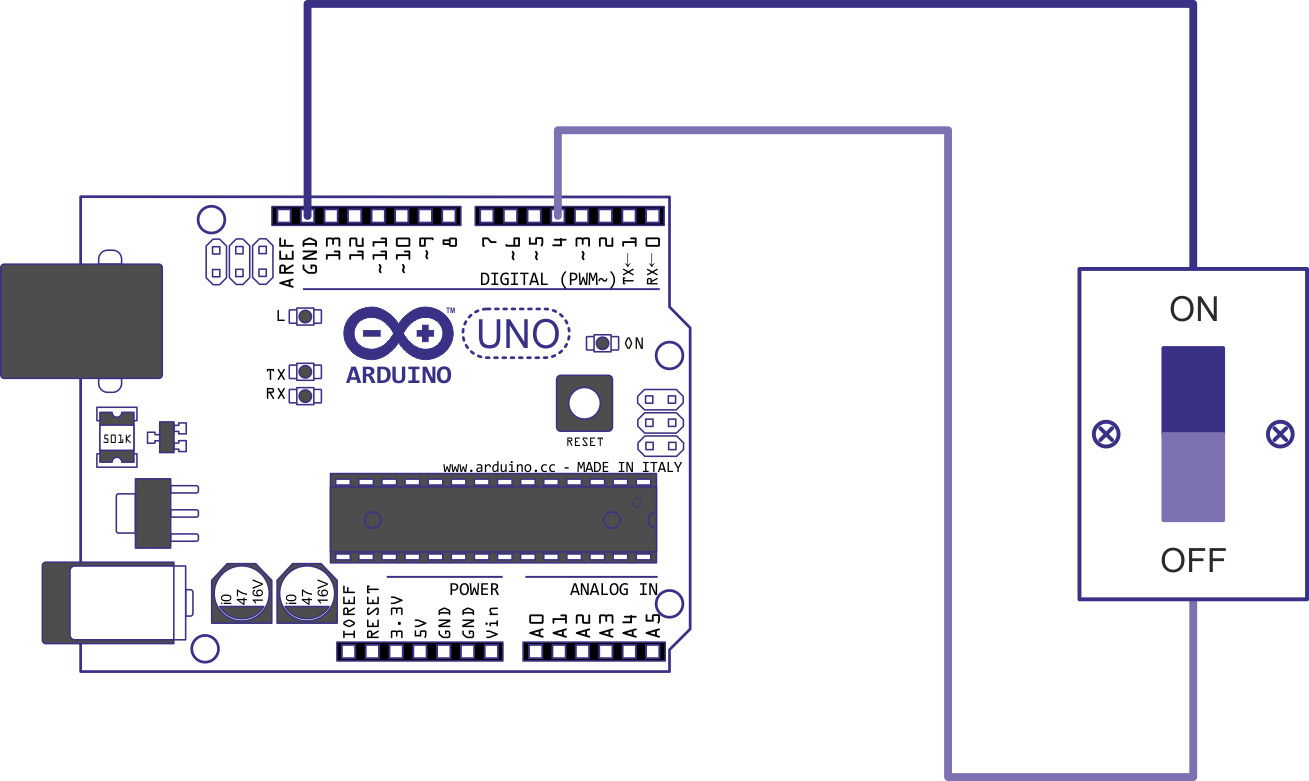
\includegraphics[width=0.8\textwidth]{imagenes/arduino_interruptor.png}
     \caption{Ejemplo de conexion Arduino y un interruptor}
     \label{fig:conexion-ard-int}
    \end{figure}
 
 
 El segundo cambio a introducir es posibilitar el accionado de las luminarias de manera digital, es decir, controlado desde el nodo. Para esto utilizaremos el circuito de la figura \ref{fig:circuito_int}. 
 
\begin{figure}[htb]
    \centering
    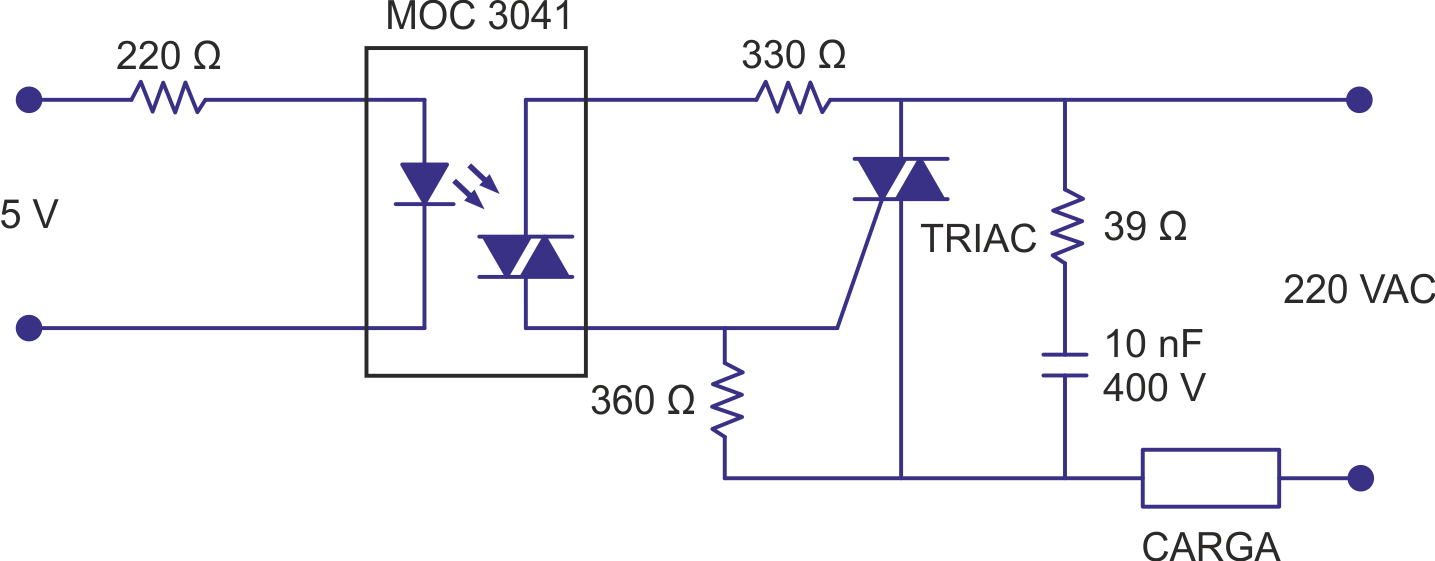
\includegraphics[width=0.8\textwidth]{imagenes/circuito_interruptor.png}
    \caption{Circuito interruptor}
    \label{fig:circuito_int}
\end{figure}
 
 Este circuito, conocido como relé de estado sólido, nos permite accionar cualquier carga eléctrica desde el nodo. Su funcionamiento es muy sencillo: el nodo activa el led dentro del optoacoplador, este hace que el triac del optoacoplador empiece a conducir, lo cual activa el triac principal, que es el que maneja realmente la carga. 
 
 Hemos elegido como optoacoplador el MOC3041 porque incorpora <<detección de paso por cero>>. El optoacoplador espera a que la señal de  alterna pase por cero para abrir o cerrar el paso de corriente. Gracias a este comportamiento se reduce el estrés en los aparatos, ya que la señal eléctrica les llega gradualmente, y se consigue una vida útil mas larga.
  
En la figura \ref{fig:ard_int_lamp} se muestra esquema de conexión entre un noodo, el relé y una lampara.

\begin{figure}[htb]
    \centering
    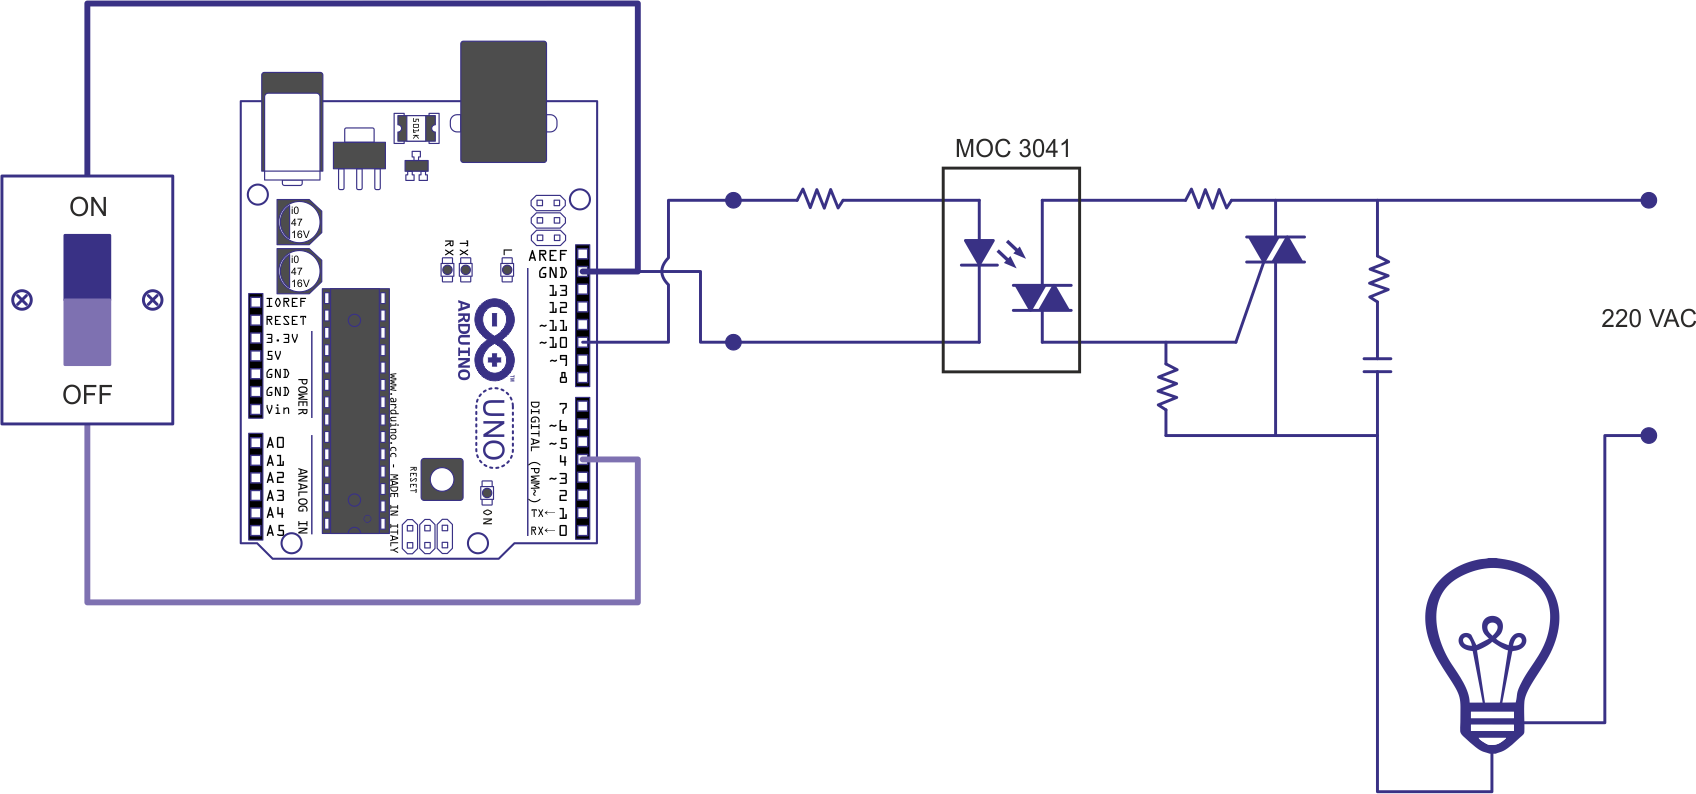
\includegraphics[width=0.8\textwidth]{imagenes/arduino_lampara.png}
    \caption{Ejemplo de conexion: Arduino, interruptor, relé y lámpara}
    \label{fig:ard_int_lamp}
\end{figure}

Cada Arduino dispone de 14 pines de entrada/salida digitales, estos son los que utilizaremos para conectar los interruptores y actuadores(relés). Los pines analógicos los reservaremos para conectar los sensores.

\subsection{Funcionamiento}

El código que se ejecuta en cada arduino consta de tres partes: <<configuración>>, <<setup>>, <<loop>>.
\subsubsection{Configuracion}
En esta parte del codigo es donde se configuran todos los parámetros que necesita arduino para funcionar.

Lo primero es definir la identificación del nodo.
\begin{lstlisting}

const char MY[] = "01";

\end{lstlisting}

Después, tenemos que especificar en que patillas están conectados los interruptores, los actuadores, y la relacion de ambos.

\begin{lstlisting}

#define NUM_INT 1
int PIN_INTERRUPTORES[NUM_INT] = {7};


int INTERRUPTOR_ACTUADOR[NUM_INT] = {0};


#define NUM_ACT 2
int PIN_ACTUADORES[NUM_ACT] = {11, 13};

\end{lstlisting}

En el array <<INTERRUPTOR\_ACTUADOR>> es donde se relacionan los interruptores con los actuadores. La posicion dentro del array hace referencia al interruptor, y el valor de dicha posicion referencia al actuador corrrespondiente. En el ejemplo mostrado, el primer interruptor esta conectado al pin 7 de arduino, y el actuador que debe accionarse es el de la posicion 0, es decir, el actuador en el pin 11.

Acto seguido se configuran los pines de los sensores, temperatura, movimiento y luz. Ademas de la posición (dentro del vector <<PIN\_ACTUADORES>>) del actuador del sensor de movimiento, y el tiempo que éste debe estar encendido en milisegundos. 

\begin{lstlisting}{breaklines=true}

int PIN_TEMPERATURA = 1;
int ARRAY_TEMPERATURA[10];


int PIN_PIR = 10;
int ACTUADOR_PIR = 0;
int TIEMPO_PIR = 3000;


int PIN_LDR = 2;
\end{lstlisting}

El resto del codigo hasta la siguiente sección, son variables globales necesarias para el correcto desarrollo de arduino. Aqui no es necesaria la configuración.

\begin{lstlisting}

// Vector de estado de interruptores

int ESTADO_INTERRUPTORES[NUM_INT];


// Vector de valores de los actuadores


int VALOR_ACTUADORES[NUM_ACT];


// Variables de control de mensajes


int FUNCION_MSJ, ACTUADOR_MSJ, VALOR_MSJ;


// Flags


int FLAG_PIR = 0;
int FLAG_MSJ = 0;

// Timers


unsigned long TIMER_INTERRUPTOR[NUM_INT];
unsigned long TIMER_PIR;

\end{lstlisting}

El array <<ESTADO\_INTERRUPTORES>> se usa para monitorizar el valor de cada interruptor, en busca de cambios entre lo almacenado y el actual, para detectar pulsaciones del usuario.

En el array <<VALOR\_ACTUADORES>> se almacena el valor de todos los actuadores.

Las variables: <<FUNCION\_MSJ>>, <<ACTUADOR\_MSJ>>, <<VALOR\_MSJ>>, se usan en las tareas de descodificación de los mensajes recibidos de la red.

Las <<flags>> se utilizan para comunicar eventos dentro del programa.

Por último tenemos los <<timers>> o temporizadores, éstos se utilizan para evitar el uso de sentencias como \lstinline[]|delay()|. En ellos se almacena el tiempo que arduino lleva encendido, funcion \lstinline|millis()|, y en sucesivas vueltas del <<loop>> se comprueba el tiempo que ha pasado.


\subsubsection{Setup}
Esta parte del código solo se ejecuta una vez, justo al encenderse el arduino.

Aqui usamos la información introducida en la <<configuración>> para ajustar los parámetros internos del microcontrolador e inicializar las comunicaciones. El código es el siguiente:

\begin{lstlisting}
void setup() {
Serial.begin(9600);
int i;

//Interruptores, inicializacion
for(i = 0; i < NUM_INT; i++){
pinMode (PIN_INTERRUPTORES[i], INPUT_PULLUP);
ESTADO_INTERRUPTORES[i] = digitalRead (PIN_INTERRUPTORES[i]);
TIMER_INTERRUPTOR[i] = 0;
}

//Actuadores, inicializacion
for(i = 0; i < NUM_ACT; i++){
pinMode(PIN_ACTUADORES[i], OUTPUT);
VALOR_ACTUADORES[i] == 0;
}

//Sensores
pinMode(PIN_PIR, INPUT);
}
\end{lstlisting}

Empieza por configurar el puerto serie a 9600 baudios. 

Luego, se configuran los pines correspondientes a los interruptores como entradas, y se activan las resistencias <<pull-up>> internas del microcontrolador. La razón de usar las resistencias internas es eliminar circuitería extra de cara al usuario.

Tambien se configuran los pines de los actuadores como salidas digitales, y los pines de los sensores como entradas.

A la vez que se configuran los pines, se inicializan los valores de los vectores <<ESTADO\_INTERRUPTORES>> Y <<VALOR\_ACTUADORES>>.

\subsubsection{Loop}
Como ya sabemos el <<loop>> es un bucle que se ejecuta sin parar y hasta el infinito dentro de arduino. Aquí es donde reside toda la lógica del nodo.

Lo hemos dividido en varias secciones, que se ejecutan en orden.

\begin{enumerate}
    \item Recepción de mensajes.
    \item Sensores e Interruptores.
    \item Actualización de actuadores.
\end{enumerate}

\subsubsection{Recepción de mensajes}
En esta parte, cada vez que se inicia de nuevo el <<loop>>, miramos si hemos recibido algo por el puerto serie. Si esto es así, llamamos a la función \lstinline|recibeMensaje()|, donde esperamos a terminar de recibir el mensaje, se descodifica y activamos la bandera de recepción de mensaje.

\begin{lstlisting}
if(Serial.available() > 0){
    recibeMensaje();
    if(FLAG_MSJ == 1){
        FLAG_MSJ = 0;
        procesaMensaje();
    }
}
\end{lstlisting}

Acto seguido, se procesa el mensaje, ejecutando la orden recibida.

\subsubsection{Sensores e interruptores}
Esta seccion se subdivide en otras dos partes: control de interruptores y lectura de sensores.

Veamos primero el control de los interruptores. El código:
\begin{lstlisting}
for(i = 0; i < NUM_INT; i++){
    est_aux = digitalRead(PIN_INTERRUPTORES[i]);

    if(est_aux != ESTADO_INTERRUPTORES[i]){
        ESTADO_INTERRUPTORES[i] = est_aux;

        if(TIMER_INTERRUPTOR[i] == 0){
            TIMER_INTERRUPTOR[i] = millis();
            cambiaActuador(INTERRUPTOR_ACTUADOR[i]);
        }
    }

    if(TIMER_INTERRUPTOR[i] != 0 && 
            (millis() - TIMER_INTERRUPTOR[i] > 1000)){
        TIMER_INTERRUPTOR[i] = 0;
    }
}
\end{lstlisting}


Como vimos anteriormente, en el escenario sobre el que trabajamos lo que tenemos son interruptores convencionales. Por ello, para controlarlos, buscamos cambios en el estado; es decir, saltos tanto de 0 a 5V como de 5 a 0V. 

Teniendo lo anterior en cuenta, el proceso es el siguiente: se recorre el array de interruptores, <<PIN\_INTERRUPTORES>>, comprobando el estado que tenemos guardado con el actual. En caso de encontrar algún cambio, guadamos el nuevo estado, activamos el timer correspondiente y llamamos a la función \lstinline|cambiaActuador()|. Esta función lo único que hace es guardar en el array <<VALOR\_ACTUADORES>> el nuevo valor, para su posterior actualización y notifica a la Raspberry el nuevo valor del actuador.


Si se ha detectado un cambio, pero el timer aun sigue activo, solo guardamos el nuevo estado para las siguientes comprobaciones. Al cabo de 1000 milisegundos, desactivamos el timer y vuelve a empezar el ciclo.

Lo siguiente en el <<loop>> es leer el valor de los sensores. Esto lo hacemos leyendo el sensor y guandando los valores sobre un array de 10 posiciones de forma cíclica. Luego, cuando se solicite el valor de alguno de los sensores, se realiza una media aritmética de los valores del array, así, se obtienen lecturas más estables.

\begin{lstlisting}
ARRAY_TEMPERATURA[bucle_sensor] = analogRead(PIN_TEMPERATURA);
//Luz
array_luz[bucle_sensor] = analogRead(PIN_LDR);


bucle_sensor = (bucle_sensor + 1) % 10;
\end{lstlisting}


Lo siguiente y último de esta parte es el control del sensor de movimiento. 

Para activar la luz del sensor de movimiento lo primer es comprobar que la bandera del sensor no este activa. Esta bandera se activa al encenderse la luz de forma explícita, sin que el sensor se active. Además, por supuesto, tiene que activarse el sensor.

Una vez el sensor se ha activado, comprobamos la cantidad de luz que hay en la habitación, ya que es posible que no haga falta encender nada. Si todo está bien, se ha activado el sensor y no hay luz suficiente, se activa el temporizador del sensor y se actualiza el valor en el array de actuadores.

En el caso de que se active el sensor, y el temporizador ya este activo, nos saltamos la comprobación de la luz, puesto si el temporizador esta activo significa que la luz esta encendida y por lo tanto esta comprobación siempre dará negativo, por que hay luz. En este caso solo reiniciamos el temporizador.

Una vez ha pasado el tiempo configurado por el usuario, desactivamos el temporizador y apagamos la luz.

El código para esto es el siguiente:

\begin{lstlisting}
if(FLAG_PIR == 0 && digitalRead(PIN_PIR) == HIGH){

    if(TIMER_PIR == 0){
        for(i = 0; i < 10; i++){
            cantidad_luz += array_luz[i];
        }
        cantidad_luz = cantidad_luz / 10;
    }else{
        cantidad_luz = 0;
    }

    if(cantidad_luz < 500){
        TIMER_PIR = millis();
        VALOR_ACTUADORES[ACTUADOR_PIR] = 1;
    }
}


if( TIMER_PIR != 0 && (millis() - TIMER_PIR > TIEMPO_PIR)){
        TIMER_PIR = 0;
        VALOR_ACTUADORES[ACTUADOR_PIR] = 0;
}
\end{lstlisting}


\subsubsection{Actualización de actuadores}
Por último se actualizan los actuadores a los valores nuevos. En el array <<VALOR\_ACTUADORES>> tenemos almacenado el valor que deben tener los actuadores, así, recorremos el array escribiendo por la salida de cada actuador su valor correspondiente. 




\begin{lstlisting}

for(i = 0; i < NUM_ACT; i++){
    if(VALOR_ACTUADORES[i] == 0){
        digitalWrite(PIN_ACTUADORES[i], LOW);
    }else{
        digitalWrite(PIN_ACTUADORES[i], HIGH);
    }
}

\end{lstlisting}

Antes de terminar, hay que destacar una característica de los nodos: el funcionamiento tanto de los interruptores físicos, como del sensor de movimiento, están programados completamente dentro de arduino. Esto quiere decir que cada uno de los nodos es completamente autónomo en el funcionamiento más básico. Aunque, por ejemplo, el router o la Raspberry no estén operativos, o se caiga la red XBee; el funcionamiento físico nunca se perderá.

\section{Estación base - Raspberry Pi}
La estación base, o la Raspberry Pi en nuestro sistema, es la encargada de gestionar todo el sistema. Desde aqui se gestionan las conexiones y se ejecutan las tareas de alto nivel.

\subsection{Ubicación}
A priori, lo ideal sería ubicar la Raspberry cerca del router doméstico, pues se supone que será un punto cercano al centro de la vivienda, y ademas se podría conectarla a el directamente con un cable Ethernet. Aunque esto no pueda ser así, tampoco es un problema ya que la conexión con la red de sensores es inalámbrica, y existe la posibilidad de añadir un dongle Wi-Fi para la conexión a la red doméstica.

\subsection{Equipamiento}

El equipamiento adicional necesario para la Raspberry solo consta de dos elementos, el resto lo trae de serie.

El primer elemento que hay que añadirle es un módulo XBee. Para ello existen en el mercado diversas opciones, como por ejemplo el módulo <<XBee Xplorer>> este permite conectar una placa XBee a un puerto USB de la Raspberry. En la fotografía de la figura \ref{fig:foto_xbeexplorer} podemos ver uno. Lo importante, más allá del producto o método utilizado, es que la conexión con el módulo XBee sea a través del puerto serie.

\begin{figure}[htbp]
    \centering
    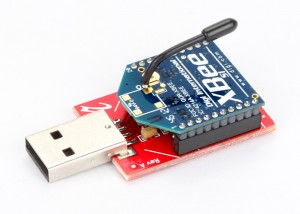
\includegraphics[width=0.80\textwidth]{imagenes/xbeexplorer.jpg}
    \caption{Módulo XBee Explorer}
    \label{fig:foto_xbeexplorer}
\end{figure}

El segundo elemento es para proporcionar conectividad con la red doméstica, esto puede ser un simple cable Ethernet, o un dongle Wi-Fi, es indiferente.


\subsection{Estructura lógica}

El funcionamiento lógico de la Raspberry está dividido en tres bloques. 

Una base de datos, que nos proporciona una estructura en la que almacenar la información necesaria para la gestión del sistema. 


Un servidor central, donde se procesan las peticiones de la aplicacion de usuario y los mensajes de la red, se envían las órdenes pertinentes y se actualiza la información de la base de datos.

Por último, la aplicación de usuario, en ésta se proporciona una interfaz gráfica para el manejo del sistema. Desde ella se activan y desactivan las luces y las escenas, se programan las acciones, etc... Además, sirve para configurar el sistema a través de la base de datos.

\subsection{Base de datos}
\begin{figure}[htbp]
    \centering
    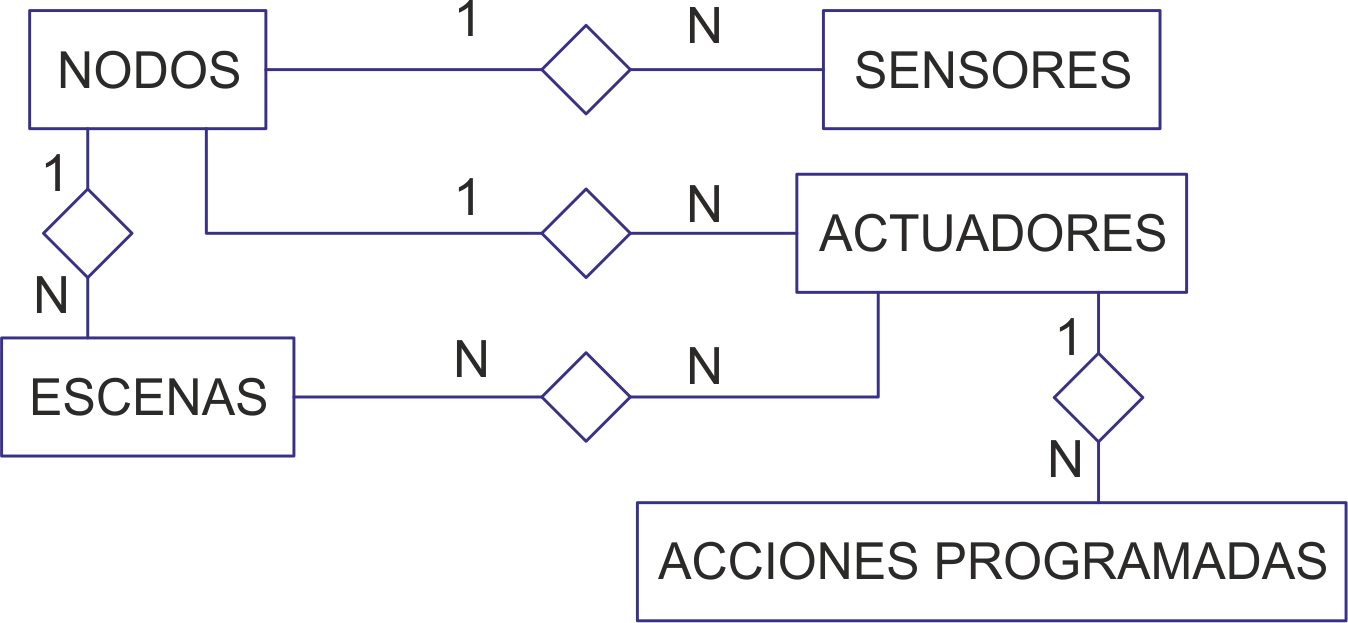
\includegraphics[width=0.80\textwidth]{imagenes/esquema_bd.png}
    \caption{Esquema de la base de datos}
    \label{fig:esquema_bd}
\end{figure}

El esquema lo podemos ver en la figura \ref{fig:esquema_bd}. La base de datos se ha diseñado para cumplir con los requisitos actuales, y que sea fácilmente ampliable en un futuro.



Las entidades que hemos considerado relevantes son:
\begin{description}
    \item[Nodos] Esta entidad hace referencia, indistintamente, a los arduinos que componen la red de sensores, y a las habitaciones donde se encuentran. Se almacenan los datos relativos a estos.
    \item[Sensores] Aquí se almacena todo lo relativo a los sensores monitorizados de los nodos. En nuestro caso, solo tenemos sensores de temperatura. 
    \item[Actuadores] Esta entidad modela las luminarias instaladas en cada nodo. 
    \item[Escenas] Éstas son las distintas configuraciones fijas de una habitación, que por alguna razón el usuario considere guardar.
    \item[Acciones programadas] En esta entidad se modela las órdenes de encendido o apagado a alguna hora determinada.
\end{description}

Estas entidades, y sus relaciones, se traducen en el siguiente conjunto de tablas.

\begin{itemize}
   \item Nodos \{id, my, estancia\}
   \item Sensores\{id, tipo\_sensor, valor, nodo\_id\}
   \item Actuadores\{id, nombre, posicion, estado, nodo\_id\}
   \item Escenas\{id, nombre, nodo\_id\}
   \item Actuador\_Escena\{escena\_id, actuador\_id, estado\}
   \item Acciones\{id, nombre, estado, actuador\_id\}
   \item Accion\_dia\{accion\_id, dia\_sem\}
\end{itemize}





\subsection{Servidor central}

 Desde el punto de vista del software, si consideramos la programación de los nodos como la capa de nivel mas bajo, y la aplicación de usuario como la de nivel mas alto, el servidor central ocupa la capa intermedia. Actúa como puente de unión o nexo entre ellas.
 
 El servidor se ha escrito desde cero, y el lenguaje elegido es Python, en su última versión. 
 
 La estructura del servidor está dividida en tres hilos: uno para la interfaz con la red de sensores, otro para la interfaz con la aplicación, y un tercero para gestionar el sistema. 
 
 
 Para las comunicaciones internas del servidor usamos varios objetos del tipo <<Queue>>. Estos objetos son un tipo de cola que permiten el paso de información entre hilos de forma eficiente, ya que trae implementado de serie los mecanismos de seguridad y control necesarios.
 
 El funcionamiento a grandes rasgos es el siguiente. 
 
 El hilo <<interfaz wsn>> esta constantemente esperando a recibir o un mensaje de la red, que lo pasa al hilo de gestión; o a recibir un mensaje para enviar a la red, que inmediatamente despues de recibirlo lo envía a través del puerto serie.
 
 El hilo <<interfaz app>> está esperando una conexión desde la aplicación de usuario, cuando la recibe, extrae la petición y se la envía al hilo de gestión.
 
 En el hilo de gestión, se procesan los mensajes de la red para actualizar la base de datos, se traducen las peticiones en mensajes para la red, y se ejecutan tareas periódicas como pedir la temperatura de las habitaciones y se establecen las alarmas para las acciones programadas.
 
 El script principal es el siguiente:
 \begin{lstlisting}
 if __name__ == "__main__":
     recibidos = queue.Queue()
     a_enviar =  queue.Queue()
     peticiones = queue.Queue()
 
     hilopcm = pcm.Pcm(recibidos, a_enviar, peticiones)
     hilopcm.start()
 
     hilowsn = interfazwsn.InterfazWsn(recibidos, a_enviar)
     hilowsn.start()
 
     hiloapp = interfazapp.InterfazApp(a_enviar, peticiones)
     hiloapp.start()
 \end{lstlisting}
 
 En este script se crean los tres objetos <<Queue>> que necesitamos.
 \begin{description}
     \item[recibidos] En esta cola se almacenan los mensajes recibidos desde la red de sensores.
     \item[a\_enviar] Aqui se almacenan los mensajes salientes hacia la red.
     \item[peticiones] En esta cola guardamos las peticiones que van llegando desde la aplicación de usuario.
    \end{description}
 
 A continuación se crean los tres hilos que manejan el sistema y se les pasan las colas que necesitan cada uno. Al <<hilowsn>>, <<recibidos>> y <<a\_enviar>>; al <<hiloapp>>, solo <<peticiones>>; y al <<hilopcm>>, las tres colas. Una vez creados se inicia su ejecución con la función \lstinline|Threading.start()|.
 
 \subsubsection{Hilo interfaz red de sensores}
 
 Este script se encarga de envolver las comunicaciones con la red de sensores. Para ello, se inicializa el puerto serie, y se monitoriza constantemente tanto el puerto serie, como la cola de envíos. 
 
 El scritp es el siguiente:
  \begin{lstlisting}
  class InterfazWsn(threading.Thread):
      def __init__(self, rec, env):
          threading.Thread.__init__(self)
          self.recibidos = rec
          self.enviar = env
      
      def run(self):
          wsn = serial.Serial("/dev/ttyACM0", 
                      baudrate=9600, timeout=1.0)
          while True:
              if wsn.inWaiting() > 0:
                  msj_b = wsn.readline()
                  msj = msj_b.decode('ascii')
                  self.recibidos.put(msj)
          
              if self.enviar.qsize() > 0 :
                  msj = self.enviar.get()
                  self.enviar.task_done()
                  msj_b = msj.encode()
                  wsn.write(msj_b)
  \end{lstlisting}
 
 
 Cuando recibe un mensaje desde la red, este está en formato <<byte>>, binario, así que lo decodifica en <<ascii>>(función \lstinline|msj_b.decode('ascii')|), y lo envía al hilo de gestión, \lstinline|recibidos.put(msj)|.
 
  Al recibir un mensaje a enviar, hace el proceso inverso. Lo convierte en formato <<byte>>, función \lstinline|msj.encode()|, lo transmite por el puerto serie, \lstinline|wsn.write(msj_b)|.
  
  
 \subsubsection{Hilo interfaz aplicación de usuario}
 
 Para este hilo hemos creado un pequeño servidor <<TCP>>. Este servidor, también basado en hilos, escucha por el puerto <<TCP 9999>> a la espera de comunicaciones de la aplicación de usuario. Cuando una de éstas llega, crea un hilo nuevo para esa conexión y vuelve a la espera.
 
 En el hilo nuevo, la aplicación comunica su petición a traves de un objeto <<JSON>>. Si éste es correcto, se pasa inmediatamente al hilo de gestión y se envía un <<ok>> de vuelta a la aplicación. En caso de no ser un <<JSON>> correcto, se obvia la petición y se manda hacia atrás un <<fail>>.
 
 El script es el siguiente:
 \begin{lstlisting}
 class InterfazApp(threading.Thread):
     def __init__(self, pet):
         threading.Thread.__init__(self)
         self.peticiones = pet
         self.a_enviar = envio
 
     def run(self):
         servidor = socket.socket(socket.AF_INET, socket.SOCK_STREAM)
         servidor.setsockopt(socket.SOL_SOCKET, socket.SO_REUSEADDR, 1)
         servidor.bind(('localhost', 9999))
         servidor.listen(5)
         i = 0
         while True:
             conn, (host, puerto) = servidor.accept()
             handler = AppHandler(conn, host, puerto, self.a_enviar, self.peticiones)
             handler.start()
         servidor.close()
 \end{lstlisting}
 
 En esta primera parte, se crea el hilo con las colas correspondientes, el socket tcp, y se pone a la escucha del puerto, \lstinline|servidor.accept()|. Cuando entra una conexión, crea el objeto que la manejará, \lstinline|AppHandler(...)|, y lo inicia.
 
 La clase que maneja la información que transmite la aplicación es la siguiente:
 \begin{lstlisting}
 class AppHandler(threading.Thread):
     def __init__(self, con, host, puerto, envia, pet):
         threading.Thread.__init__(self)
         self.conexion = con
         self.peticiones = pet
         self.host = host
         self.puerto = puerto
         self.a_enviar = envia
 
     def run(self):
         data  = self.conexion.recv(1024)
         data = data.decode('UTF-8')
         deco  = json.loads(data)
         respuesta = ""
 
         if ('peticion' in deco):
             self.peticiones.put(deco)
             respuesta = '{ ok : 1 }'
             else:
             respuesta = '{ fail : 0 }'
 
 
         response = json.dumps(respuesta)
 
         self.conexion.send(bytes(response, 'utf8'))
 
         self.conexion.close()
 \end{lstlisting}
 
Una vez creado el objeto, recibe los datos, los descodifica (\lstinline|deco=json.loads(data)|) en  <<JSON>>, y se comprueba que exista el campo <<peticion>>. Si esto es así, encola la petición, \lstinline|peticiones.put(deco)|, crea el <<ok>> de respuesta y lo envía, y cierra la conexión. Si el <<JSON>> no contuviera el campo <<peticion>>, significa que no es una petición válida, por lo que creará una respuesta <<fail>> y la enviará. 

El motivo de realizar las comunicaciones entre el servidor en Python y la aplicación de usuario a través de conexiones <<TCP>> es flexibilizar el sistema. De esta manera, se puede descentralizar la aplicación y ésta podría estar ejecutandose en otra máquina. O por ejemplo, crear una aplicación específica para un sistema operativo, y que ésta siga teniendo acceso al sistema. Además, los objetos <<JSON>> son casi un estándar de facto en las comunicaciones entre aplicaciones, con lo que, crear estas aplicaciones alternativas no deberiía ser un problema.


\subsubsection{Hilo de gestión}

En este hilo es donde reside la mayor parte de la lógica del servidor. El script está dividido estructuralmente en tres partes: tratamiento de mensajes de la red, tratamiento de peticiones de la aplicación y acciones periódicas.

El scrip se inicia con el constructor de la clase. En éste se crean las variable para albergar las colas de comunicación, se abre la conexión con la base de datos, y por último se crea el array que contendrá los objetos <<Timer>>.

\begin{lstlisting}
class Pcm(threading.Thread):
    def __init__(self, rec, env, pet):
        threading.Thread.__init__(self)
        self.recibidos = rec
        self.enviar = env
        self.peticiones = pet
        self.bd = pymysql.connect(host='127.0.0.1', 
                                  port=3306,
                                  user='root', 
                                  passwd='xxxxx', 
                                  db='platymo')
        self.timers = []
\end{lstlisting}

El objeto <<Timer>> es un objeto especial de la clase <<Threading>>, la clase encargada de los hilos de ejecución en Python. Al constructor de este objeto se le pasa una cantidad de tiempo, en segundos, y una función. Al cabo ese tiempo ejecuta la función y se destruye. En nuestro sistema, éstos objetos se utilizan para programar envíos de mensajes en diferido, las acciones programadas del sistema. 

El código para el procesado de los mensajes de la red es el siguiente:
\begin{lstlisting}
if self.recibidos.qsize() > 0 :
    msj = self.recibidos.get()
    self.recibidos.task_done()

    my = msj[:2]
    func = msj[2:4]
    act = msj[4:6]
    val = msj[6:9]

    if func == "10":
        self.setValBDActuador(my, act, val)
    elif func == "20":
        self.setValBDSensor(my, act, val)
    elif func == "00":
        self.setApagarTodo(my)
\end{lstlisting}

Cuando se recibe un mensaje, se descodifica y dependiendo de su contenido se aplica una función u otra. 

\begin{description}
    \item[setValBDActuador(my, act, val)] Actualiza el valor del actuador en la base de datos.
    \item[setValBDSensor(my, act, val)] Actualiza el valor del sensor en la base de datos.
    \item[setApagarTodo(my)] Actualiza todos los actuadores del nodo en cuestión al valor 0.
\end{description}


Para el procesamiento de las peticiones de la aplicación, el método a seguir es análogo al anterior.
\begin{lstlisting}
if self.peticiones.qsize() > 0:
    peticion = self.peticiones.get()
    self.peticiones.task_done()

    if peticion['peticion'] == "actuador":
        self.setActuador(peticion['id'], peticion['valor'])
    elif peticion['peticion'] == "escena":
        self.activarEscena(peticion['escena'])
    elif peticion['peticion'] == "apagarTodo":
        self.apagarTodo()
    elif peticion['peticion'] == "actualizarTimers":
        self.setTimers()
\end{lstlisting}
 
 \begin{description}
     \item[ setActuador(peticion('id'), peticion('valor')) ] Envía a la red el mensaje correspondiente para activar o desactivar el actuador.
     \item[activarEscena(peticion('escena'))] Esta función accede a la configuración de la escena, guadada en la base de datos, y envía los mensajes correspondientes.
     \item[apagarTodo()] Envía el mensaje <<000000000>>, que activa el apagado de todos los actuadores en todos los nodos.
     \item[setTimers()] Esta función busca en la base de datos todas las acciones programadas para el día actual, y posteriores a la hora actual. Con esta información crea los objetos <<Timer>> necesarios.  A esta función se la llama cada vez que una <<acción programada>> es creada o modificada en la aplicación.
    \end{description}
    
    
 La última parte del script realizamos todas las gestiones dependientes del tiempo. Éstas son: cada 5 minutos actualizar el valor de los sensores de temperatura y  a las 00:00 de cada día crear los <<Timers>> correspondientes.
 
 El código:
 \begin{lstlisting}
 fechahora = time.localtime()
 minmodulo = fechahora[4] % 10
 
 if (minmodulo == 0 or minmodulo == 5):
     if flag_temperatura:
         self.peticionTemperatura()
         flag_temperatura = False
     else:
         flag_temperatura = True
 
 if (fechahora[3] == 0 and fechahora[4] == 0):
     if flag_timers:
         self.setTimers()
         flag_timers = False
     else:
         flag_timers = True
 \end{lstlisting}
    
  La secuencia es la siguiente: guardamos la hora actual, y si los minutos acaban en 0 o 5 simplemente se pide a todos los nodos de la red que reporten el valor del sensor de temperatura. Cuando los mensajes de respuesta de éstos lleguen, la parte del código de tratamiento de mensajes es la encargada de guardar la información.
  
  Después, comprobamos si son las 00:00, en caso afirmativo, llamamos a la función \lstinline|setTimers()| para crear los <<Timers>> correspondientes y dejar el sistema listo para el día que empieza.
  
  Las variables <<flag\_timers>> y <<flag\_temperatura>> se utilizan para que el script ejecute una sola vez las órdenes dentro del minuto correspondiente.
  
  
  \subsection{Aplicación de usuario}
  
  La aplicación de usuario es la última capa de software. Actúa como interfaz para el manejo diario del sistema y como método de configuración. Se ha escrito como una aplicación web para que el acceso sea mas universal, así, se puede acceder a ella desde ordenadores personales, teléfonos inteligentes, o tabletas.
  
  Como se ha podido observar, desde el servidor en Python solo se accede a la base de datos para extraer o actualizar información. Es desde la aplicación desde donde se inicializa o se introduce información nueva. Para el usuario final es más sencillo, y además está más acostumbrado, tratar con formularios web que, por ejemplo,  con la linea de comandos o programas específicos para bases de datos.
  
  La aplicación está escrita en PHP, concretamente usando el framework Laravel. Éste framework implementa el patrón MVC, lo que nos da una estructura, tanto de archivos como lógica, ya definida.
  
  En Laravel todo empieza con las <<rutas>>, éstas son unas URLs, definidas previamente, que se encargan de dirigir la aplicación a un controlador u otro. En los controladores se prepara la información, accediendo a los modelos de la base de datos tanto para crear nuevos, como para actualizarlos. Después, esta información se pasa a las vistas, que es lo que ve el usuario.
  
  Para las vistas, usaremos también un framework, Bootstrap, esto nos ofrece dos grandes ventajas principalmente:
  \begin{enumerate}
      \item Bootstrap incluye un sistema de rejilla para la disposición de los elementos, completamente enfocado al diseño responsable. Esto propicia que la aplicación se muestre correctamente sea cual sea el tamaño de la pantalla.
      \item También incluye una serie de elementos de interfaz definidos y listos para usar, con lo que el desarrollo es más rápido, y nos asegura un aspecto uniforme en toda la aplicación.
    \end{enumerate}
    
 En resumen, necesitamos crear: los modelos de la base de datos,  los controladores, las vistas y definir las rutas de cada pantalla de la aplicación.
 
 Conceptualmente, la aplicación se divide en dos partes: la zona de configuración, donde se crean y editan los distintos elementos del sistema, y la zona principal, donde se encienden y apagan los actuadores, se activan las escenas, en definitiva, el manejo diario.
 
 Lo primero que veamos serán los modelos, puesto que son de uso común en toda la aplicación.
 
 
 \subsubsection{Modelos}
 
 Si recordamos el esquema de la base de datos, figura \ref{fig:esquema_bd}, se ha creado un modelo por cada una de las entidades. Estos son:
 \begin{itemize}
     \item Nodo
     \item Actuador
     \item Sensor
     \item Escena
     \item Accion
    \end{itemize}
    
    Como ejemplo de la implementación de los modelos, veamos el código del modelo del nodo.
    
    \begin{lstlisting}
    class Nodo extends Model {
    
        protected $table = 'nodos';
    
        public function sensores(){
            return $this->hasMany('App\Sensor');
        }
    
        public function actuadores(){
            return $this->hasMany('App\Actuador');
        }
    
        public function escenas(){
            return $this->hasMany('App\Escena');
        }
    }
    \end{lstlisting}
    
    Primero se establece que tabla de la base de datos contiene al modelo. El ORM de Laravel automáticamente hace accesible todos los campos que contenga la tabla, solo hay que decirle las relaciones que existen con los demas modelos. Para esto, se crean las funciones que siguen.
    
    En este caso, como todas las relaciones del nodo son <<uno a varios>>, se utiliza la función \lstinline|hasMany('Modelo')|. Esta función es la que establece la relación <<uno a varios>> dentro del ORM.
    
    Para establecer la relación inversa, en el modelo del actuador, por ejemplo, se debe crear otro método, pero esta vez la función a utilizar es \lstinline|belongsTo('Modelo')|. El codigo sería:
    \begin{lstlisting}
    class Actuador extends Model {
    
        protected $table = 'actuadores';
        
        public function nodo(){
            return $this->belongsTo('App\Nodo');
        }
        
        public function acciones(){
            return $this->hasMany('App\Accion');
        }
        
        public function escenas(){
            return $this->belongsToMany('App\Escena');
        }
    }
    \end{lstlisting}
    
    A partir de este momento, desde cada objeto <<Nodo>> se podrá acceder a los sensores, actuadores y escenas asociados, y  a la inversa.
    
    El resto de modelos siguen la misma estructura.
    
    \subsubsection{Zona principal}
    
    Esta zona es el punto de entrada del usuario. 
    
    La primera pantalla, <<panel principal>>, da acceso a todas las demas partes de la aplicación. Su aspecto se puede ver en la figura \ref{fig:panel_ppal}
    
    \begin{figure}[htbp]
        \centering
        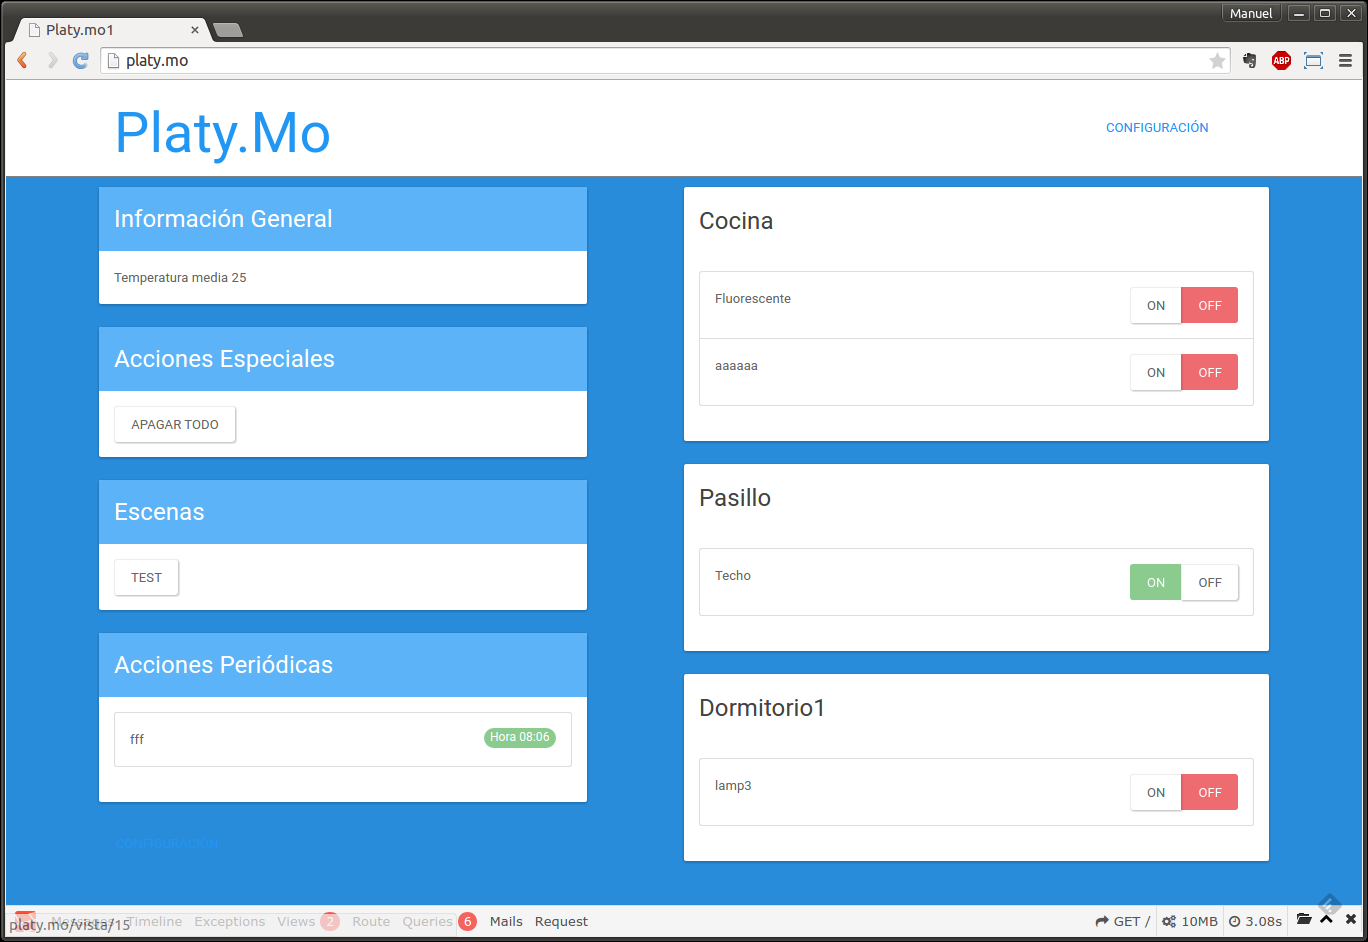
\includegraphics[width=0.95\textwidth]{imagenes/panel_ppal.png}
        \caption{Panel principal}
        \label{fig:panel_ppal}
    \end{figure}
    
    Esta pantalla esta dividida en dos columnas.
    
     A la izquierda, información general, acceso a las funciones especiales y las escenas, y una lista con todas las acciones programadas que existan. En la lista de las acciones programadas, el color de fondo donde se muestra la hora indica si se enciende o se apaga, verde y rojo respectivamente. Tanto las funciones especiales, como las escenas son botones para activarlas.
     
     A la derecha, tenemos un panel para cada habitación, en este panel se pueden accionar algunas luminarias de la habitación, estos botones también sirven como indicadores de su estado actual. Y, si pulsamos en la parte superior del panel, nos llevará a la vista detallada de la habitación. 
    
    En la esquina superior derecha, encontramos el enlace hacia la configuración. De esta zona hablaremos mas adelante.
    
   Toda esta zona esta gestionada por un único controlador, <<PrincipalController>>. En éste, se definen tres métodos: \lstinline|home()|,  \lstinline|vista()|, \lstinline|configuracion()|. Cada uno de ellos da paso a: el panel principal, la vista detallada de las habitaciones, y el panel de configuración, respectivamente. Para la zona en la que estamos, solo nos fijaremos en las dos primeras.
    
    Las rutas que definen esta parte son:
    \begin{lstlisting}
    Route::get('/', 'PrincipalController@home');
    Route::get('vista/{id}', 'PrincipalController@vista');
    \end{lstlisting}
    
    Como podemos observar, la ruta <</>> activa el método \lstinline|home()| que nos renderiza la pantalla que acabamos de ver. Su codigo:
    \begin{lstlisting}
    public function home(){
    
        $habitaciones = Nodo::all();
        $array_panel = array();
        $i = 0;
        
        foreach ($habitaciones as $habitacion) {
            $array_panel[$i] = array();
            $array_panel[$i]['habitacion'] = $habitacion;
            $array_panel[$i]['actuadores'] = array();
            $j = 0;
            foreach ($habitacion->actuadores()
                    ->where('principal', 1)->get() as $act) {
                    
                $array_panel[$i]['actuadores'][$j] = $act;
                $j++;
        }
            $i++;
        }
        
        $escenas = Escena::all();
        $acciones = Accion::all();
        
        
        
        return view('home.principal')->
                    with(array('panel' => $array_panel,
                              'escenas' => $escenas,
                              'acciones' => $acciones,
                              'title' => ''));
    }
    \end{lstlisting}
    
    En el código, primero se prepara toda la información necesaria, y después, retorna la vista correspondiente añadiendole la información recavada.
    
    De forma análoga a la anterior, la función \lstinline|vista($id)|, muestra la pantalla <<vista detallada>>, figura \ref{fig:vista_hab}; cuando se accede a la ruta <</vista/{id}>>, siendo \{id\} una variable que contiene el id de la habitacion o nodo. Hay que destacar, que esta variable es extraida de la URL.
    
     \begin{figure}[htbp]
         \centering
         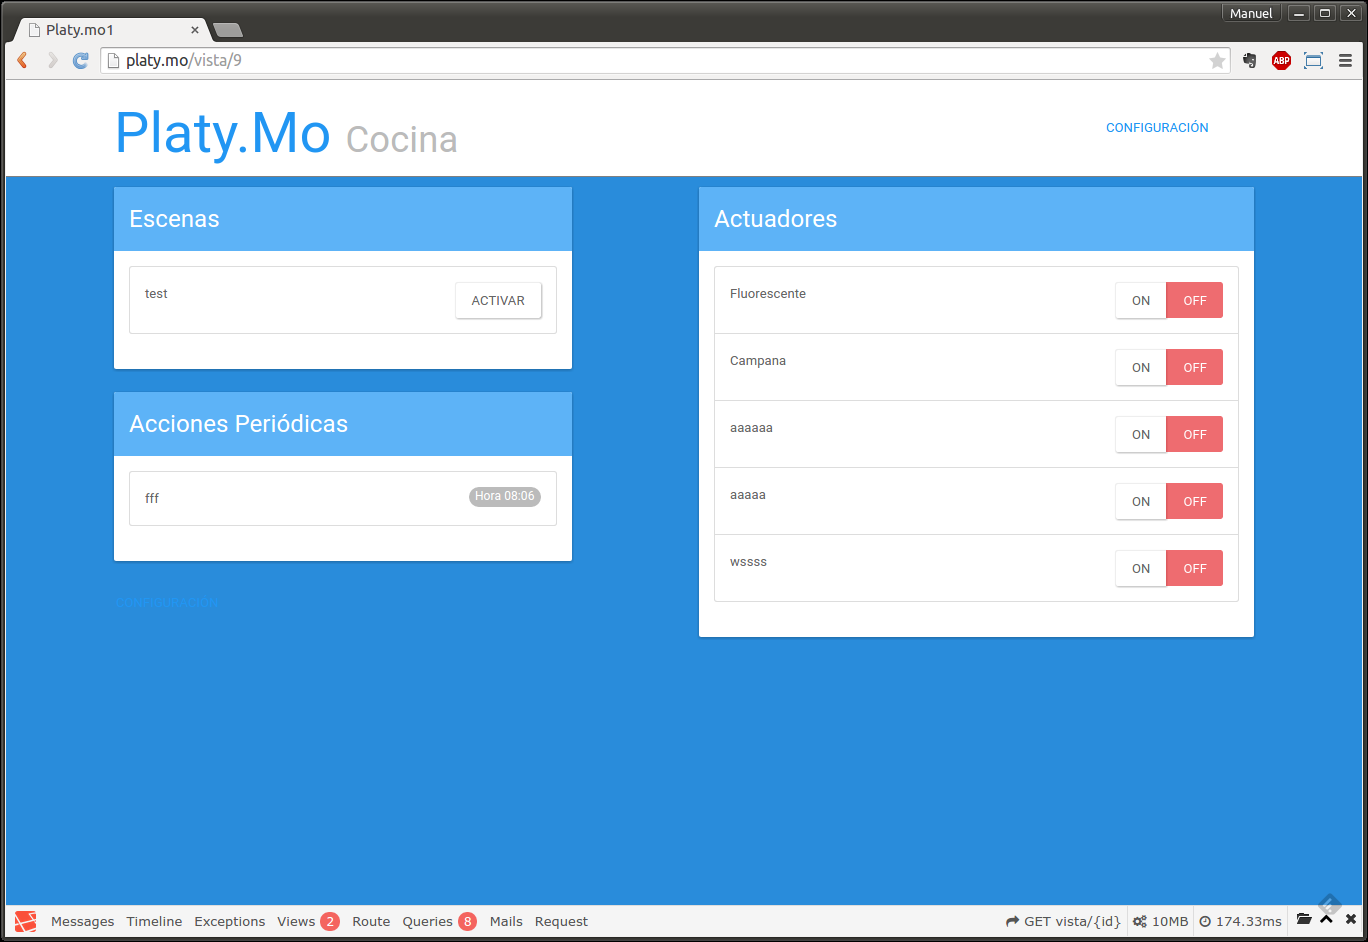
\includegraphics[width=0.95\textwidth]{imagenes/vista.png}
         \caption{Vista detallada de las habitaciones}
         \label{fig:vista_hab}
        \end{figure}
        
        
    En esta pantalla podemos ver toda la información relativa a la  habitación: las escenas y acciones configuradas y la lista completa de luminarias instaladas. 
    
    Cuando pulsamos en algún botón para activar algo, tanto en el panel principal como en las habitaciones, realmente lo que hacemos es pulsar sobre un enlace. Este enlace nos lleva a un controlador creado explícitamente para enviar las peticiones al servidor en Python, <<ComandoController>>
    
    Las rutas definidas para <<ComandoController>> son:
    \begin{lstlisting}
    Route::get('comando/actuador/{id}/{valor}',
                         'ComandoController@actuador');
                 
    Route::get('comando/escena/{id}',
                         'ComandoController@escena');
                 
    Route::get('comando/apagar', 
                        'ComandoController@apagarTodo');
    \end{lstlisting}
    
    Tomemos como ejemplo <</comando/actuador/\{4\}/\{0\}>>, en esta ruta pondríamos el actuador con id igual a 4, a valor 0, es decir, apagar el actuador 4. Para ello, la función \lstinline|actuador($id, $valor)| de <<ComandoController>> hace lo siguiente.
    
    \begin{lstlisting}
    public function actuador($id, $valor){
        $datos = array();
    
        $actuador = Actuador::find($id);
    
    
        $datos['peticion'] = 'actuador';
    
        $datos['id'] = $actuador->id;
        $datos['valor'] = (int)$valor;
    
        PythonComm::envia($datos);
    
    
        return redirect()->back();
    }
    \end{lstlisting}
    
    Se crea un array de claves con los valores: <<petición>>, actuador; <<id>>, id del actuador, <<valor>>, el valor deseado. En nuestro ejemplo quedaría como muestra la tabla \ref{tab:pet_ejem}.
    
    \begin{table}[h]
        \centering
        \begin{tabular}{c|c}
            \toprule
            peticion & actuador  \\ 
            id & 4       \\ 
            valor & 0    \\\bottomrule
        \end{tabular}
        \caption{Petición de ejemplo}
        \label{tab:pet_ejem}
    \end{table}
    
    Una vez montado el array, se llama a la función \lstinline|envia($datos)| de la librería <<PythonComm>>. Esta librería, se encarga de enviar datos hacia el servidor Python. Una vez enviados los datos, se redirecciona al usuario hacia la pantalla desde la que activara el botón, \lstinline|redirect()->back()|.
    
    En la función \lstinline|envia($datos)|, simplemente se abre un socket, el array <<\$datos>> se codifica en <<JSON>>, se envian por el socket, y se cierra la conexión. 
    
    El resto de las funciones de <<ComandoController>> funcionan de la misma forma, solo que cambiando los datos de la petición.
    
   
    \subsubsection{Zona de configuración}
    
    La zona de configuración esta construida como una serie de formularios web, a los que se accede desde un panel principal. Se accede a través de la ruta <</configuracion>>, que activa el método \lstinline|configuracion()| del <<PrincipalController>>. El proceso es el mismo, se preparan los datos necesarios, y se renderiza la vista, figura \ref{fig:panel_config}.
    
     \begin{figure}[htbp]
         \centering
         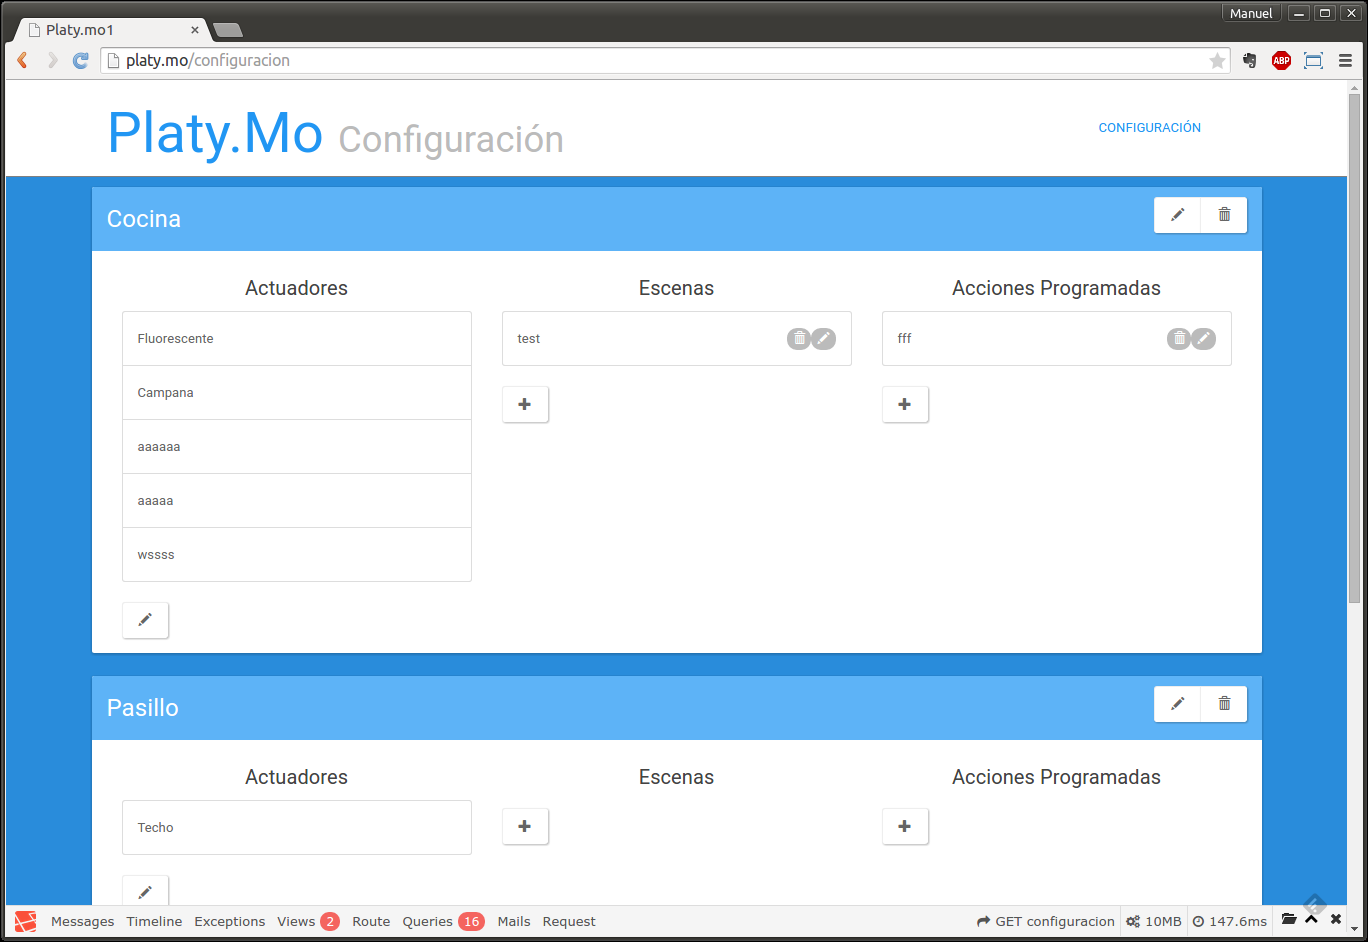
\includegraphics[width=0.95\textwidth]{imagenes/panel_config.png}
         \caption{Panel de configuración}
         \label{fig:panel_config}
        \end{figure}
        
    Este panel se organiza en función de las habitaciones que existan en el sistema. Una tarjeta para cada una de ellas. Estas tarjetas, se dividen en tres partes: lista de actuadores o luminarias, lista de escenas, y lista de acciones programadas.
    
    Como se puede observar en la captura de pantalla, cada panel habitación tiene dos botones en la parte superior derecha, para editar o borrar la habitación al completo. Abajo del todo de la pantalla, encontramos el botón <<Nueva Habitación>>, con él, creamos una nueva habitación. 
    
    Cada escena y cada acción tienen dos botones a su derecha, borrado y edición. El botón <<+>> creará una escena o acción nueva según el que pulsemos.
    
    El formulario para añadir o editar una habitación, es el que se muestra en la figura \ref{fig:form_hab}. En él introduciremos tanto la información de la habitación, <<my>> del nodo, y el nombre de ésta, como los actuadores correspondientes, su nombre, la posición dentro del array <<PIN\_ACTUADORES>>en el código del arduino, y si queremos que se muestre en el panel principal o no.
    
    
    
        \begin{figure}[h!]
            \centering
            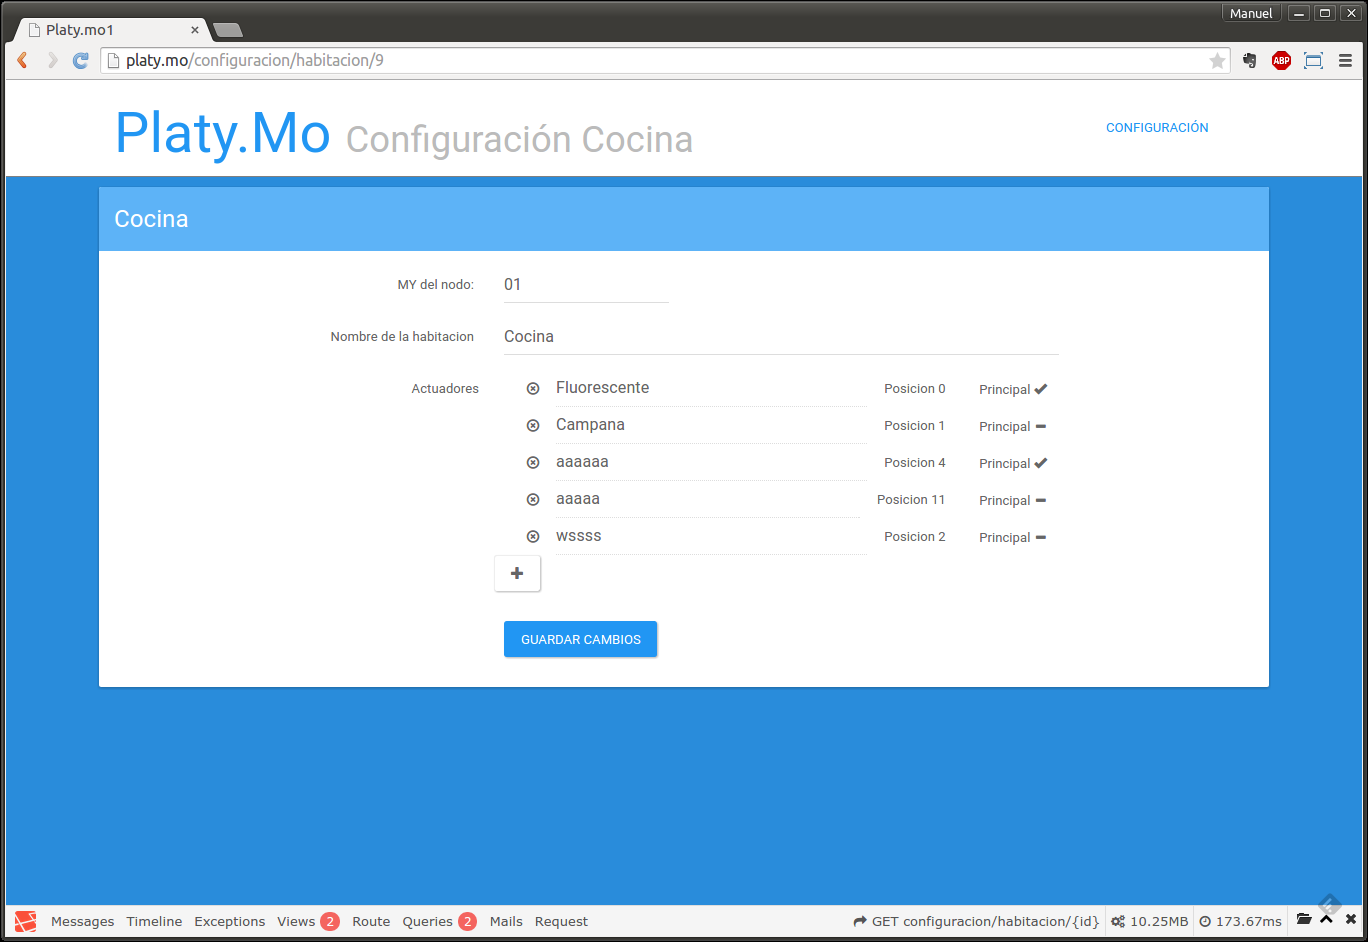
\includegraphics[width=0.95\textwidth]{imagenes/conf_hab.png}
            \caption{Formulario habitación}
            \label{fig:form_hab}
        \end{figure}
        
     Los actuadores se añaden de uno en uno. Una vez rellenados los campos correspondientes, se pulsa en el botón <<disquete>>, entonces los campos del actuador desaparecen, para mostrarse en la lista de los actuadores ya añadidos. Si quisiéramos añadir otro, pulsamos en el botón <<+>> y se creará otro juego vacío de campos para un actuador nuevo.
     
     En la lista de actuadores podemos ver los datos relativos a cada uno, y un enlace a la izquierda de cada uno para borrarlos.
     
          
     En el formulario para las escenas, introduciremos un nombre para ésta, y la configuración de luces que queramos, figura \ref{fig:form_esc}
    
    \begin{figure}[h!]
        \centering
        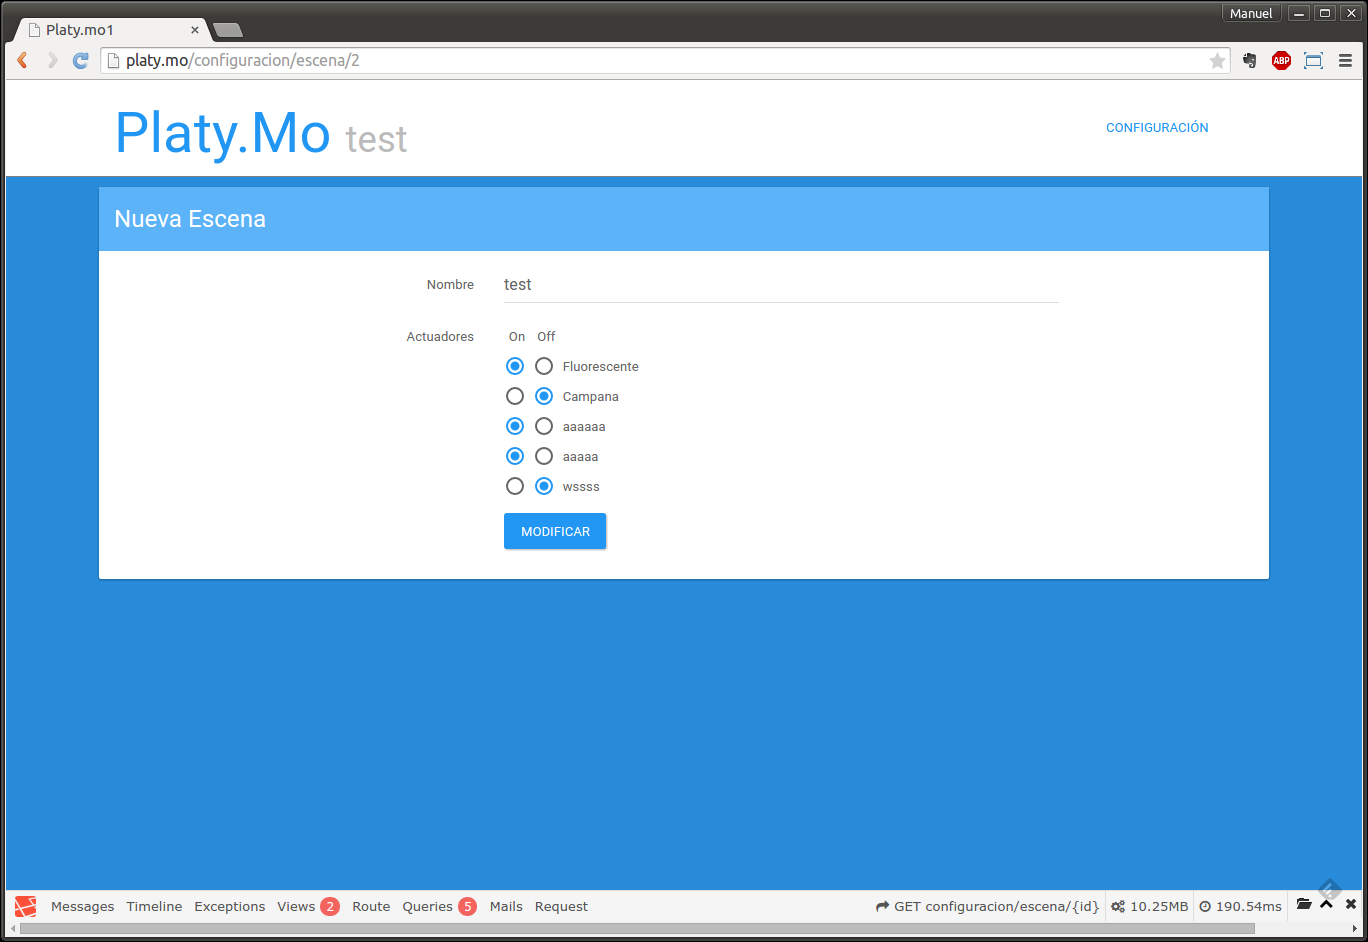
\includegraphics[width=0.95\textwidth]{imagenes/conf_esc.png}
        \caption{Formulario escena}
        \label{fig:form_esc}
    \end{figure}
    
    Por último, en el formulario para las acciones programadas veremos campos para: el nombre de la acción, el actuador que se programa, los dias de la semana que queramos q se active, la hora, y si queremos que se encienda o apague.
    
    \begin{figure}[h!]
        \centering
        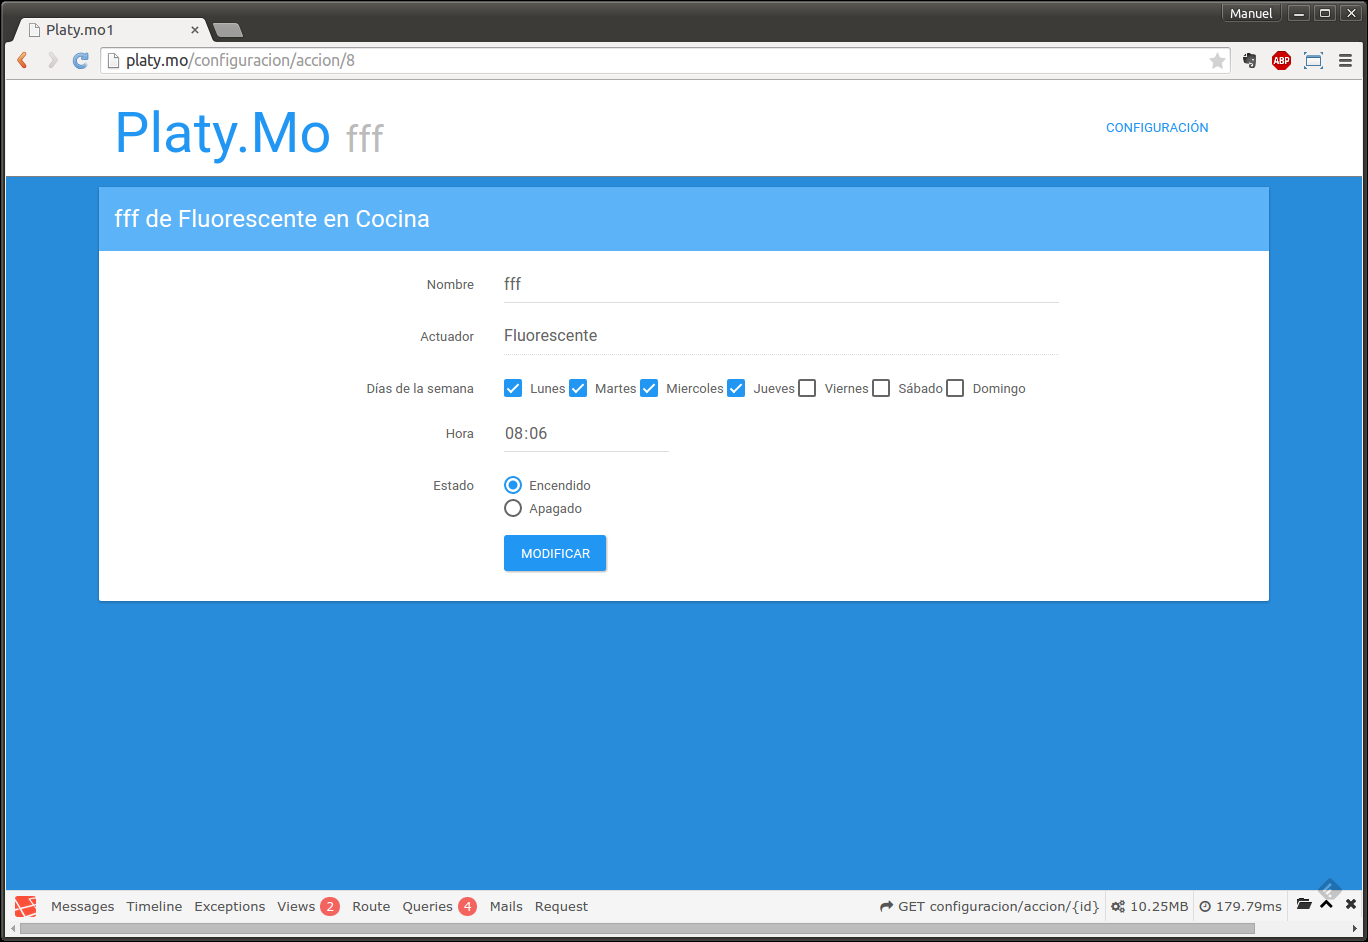
\includegraphics[width=0.95\textwidth]{imagenes/conf_accion.png}
        \caption{Formulario acción programada}
        \label{fig:form_acc}
    \end{figure}
    
    
    
  Para la gestión de todas las vistas y formularios, hemos creado diversos controladores.
    
    \begin{description}
        \item[HabitacionController] Actuadores y nodos.
        \item[EscenaController] Escenas.
        \item[AccionController] Acciones programadas.
    \end{description}
    
    El funcionamiento es similar para los tres controladores. Se crean 5 métodos, \lstinline|create()| y \lstinline|edit()| muestran los formularios, con \lstinline|store()| y \lstinline|update()| se procesan, y \lstinline|delete()| elimina el objeto en cuestión.
    
    Para mostrar el ciclo de funcionamiento, tomaremos como ejemplo el <<EscenaController>>.
    
    Al igual que antes, todo empieza con las rutas. En este caso tenemos:
    
    \begin{lstlisting}
Route::get('configuracion/habitacion/escena/{hab_id}', 
                    'EscenaController@create');

Route::post('configuracion/escena/store', 
                    'EscenaController@store');

Route::get('configuracion/escena/{id}',
                     'EscenaController@edit');

Route::post('configuracion/escena/update', 
                    'EscenaController@update');

Route::get('configuracion/escena/delete/{id}', 
                    'EscenaController@delete');
    
    \end{lstlisting}
    
    La primera de ellas, <</configuracion/habitacion/escena/\{hab\_id\}>>, renderiza el formulario para la creación de una escena nueva, en la habitación cuyo id sea <<hab\_id>>. El método encargado es \lstinline|create()|.
    
\begin{lstlisting}
public function create($hab_id){

    $habitacion = Nodo::find($hab_id);
    $actuadores = $habitacion->actuadores()->get();
    
    return view('config.escena')
        ->with(array('habitacion' => $habitacion,
                     'actuadores' => $actuadores,
                     'title' => 'Nueva escena'));
}
\end{lstlisting}
   
   El formulario creado, enviará la información recavada a <</configuracion/escena/store>>, según su ruta, se llamará al método \lstinline|store()|.
   
   \begin{lstlisting}
public function store(EscStoreFormRequest $request){

    $nodo = Nodo::find($request->get('hab_id'));
    
    $escena = new Escena;
    $escena->nombre = $request->get('nombre');
    
    $nodo->escenas()->save($escena);
    
    foreach ($nodo->actuadores()->get() as $actuador) {
        $estado = $request->get($actuador->id);
        $escena->actuadores()->
                attach($actuador->id, ['estado' => $estado]);
    }
  
    Session::flash('msg', 'Escena creada');
    return redirect('configuracion');
}
   \end{lstlisting}
   
   Aquí, podemos ver una de las características más útiles de Laravel, el sistema de validación. La variable que se introduce en la declaración del método es de una clase creada por nosotros <<EscStoreFormRequest>>, que hereda de la clase <<Request>>. Al introducir nuestra clase en la declaración, Laravel intercepta la petición, y antes de pasarla al método, le aplica las reglas de validación que incluyamos en nuestra clase. 
   
   Si no pasase la validación, Laravel automáticamente vuelve al formulario con los datos introducidos, y los mensajes de error pertinentes. Nunca llegaría al método \lstinline|store()|.
   
   \begin{lstlisting}
class EscStoreFormRequest extends Request {
    public function rules()
    {
        $rules = array(
        'nombre' => 'required|string|max:50'
        );
    
        return $rules;
    }
    
    public function messages(){
    
        return [
        'required' => 'El campo :attribute es obligatorio.',
        
        'string'=>'Solo se permiten caracteres 
                alfanumericos en el campo :attribute.',
                
        'max:50'=>'El campo :attribure puede tener como
                 maximo 50 caracteres.'
        ];
    }

}
    \end{lstlisting}
   
   Con la función \lstinline|rules()| se especifican las reglas de validación, y con \lstinline|messages()| se personalizan los mensajes de error. Lo último, es necesario, puesto que, Laravel por defecto todos los mensajes están escritos para angloparlantes.
   
   Si pasa la validación, entra en el método \lstinline|store()|. Creamos una escena nueva, se rellena y se guarda en  la base de datos.
   
   Otra característica de Laravel que podemos ver aquí, es la facilidad con la que se maneja la base de datos. En las escenas, al guardar una, también tenemos que guardar la configuración de los actuadores. Esto se realiza sobre una tabla pivote, en la que guardamos los id de ambas entidades junto con el valor que debe tomar el actuador. Lo que en principio puede ser una consulta más compleja, en Laravel simplemente llamamos a la función \lstinline|attach()|, esta función se encarga de todo por nosotros.
   
   Para la edición, procedemos de la misma forma. Con \lstinline|edit()| extraemos los datos y renderizamos el formulario. Más tarde, en \lstinline|update()|, tras pasar la validación, recuperamos la escena, modificamos los valores y guardamos.
   
   \begin{lstlisting}
public function edit($id){

   $escena = Escena::find($id);
   
   $habitacion = Nodo::find($escena->nodo()->first()->id);
   $actuadores = $habitacion->actuadores()->get();
   
   $query = DB::table('actuador_escena')
           ->where('escena_id', $escena->id)->get();
           
   $act_estado = array();
   $i = 0;
   foreach ($actuadores as $actuador) {
       $act_estado[$i] = array();
       $act_estado[$i]['id_actuador'] = $actuador->id;
       $act_estado[$i]['nombre'] = $actuador->nombre;
   
       foreach ($query as $row) {
   
           if($actuador->id == $row->actuador_id){
               $act_estado[$i]['estado'] = $row->estado;
           }
       }
       $i++;
   }





    return view('config.escenaEdit')
            ->with(array('habitacion' => $habitacion,
                'act_estado' => $act_estado,
                'escena' => $escena,
                'title' => $escena->nombre));
}


public function update(EscStoreFormRequest $request){

    $escena = Escena::find($request->get('esc_id'));
    $escena->nombre = $request->get('nombre');
    $escena->save();
    
    $data_sync = array();
    
    foreach (Nodo::find($escena->nodo_id)
                ->actuadores()->get() as $actuador) {
                
        $data_sync[$actuador->id] = 
                ['estado' => $request->get($actuador->id)];
    }
    
    $escena->actuadores()->sync($data_sync);
    
    Session::flash('msg', 'Escena modificada.');
    return redirect('configuracion');

}
\end{lstlisting}

En el método update hay que resaltar el uso de la función \lstinline|sync()|. Esta función sirve para sincronizar tablas pivote. Recibe un array con los id de una de las entidades implicadas, y actúa sobre la tabla para que solo contenga a estos id, ya sea borrando filas o añadiendo.

En nuestro caso, recibe un array con los id de los actuadores y el valor de estos, con lo que al final, la tabla queda actualizada con los nuevos datos.


Para terminar, queda la acción de borrar escenas. Gracias a Laravel y su ORM, es muy sencillo. Traemos de la base de datos el objeto a borrar, y llamamos a su función \lstinline|delete()|.
\begin{lstlisting}



public function delete($id){

    $escena = Escena::find($id);
    $escena->delete();

    Session::flash('msg', 'Escena borrada.');
    return redirect('configuracion');
}
   \end{lstlisting}
   
   
   
   
   
    
    
    
    
    
    
    
  
  
  
  
  
  
  
 
 










\end{document}